\RequirePackage[l2tabu, orthodox]{nag}

\documentclass[12pt,a4paper,dutch]{report}

\usepackage[dutch]{babel}

\usepackage{amsmath}
\usepackage{amssymb}
\usepackage{amsthm}

\theoremstyle{definition}
\newtheorem{definition}{Definitie}[section]

\usepackage{microtype}

\usepackage{url}
\usepackage{graphicx}

\usepackage[utf8]{inputenc}
\usepackage[T1]{fontenc}

\usepackage{float}
\usepackage{listings}
\usepackage{inconsolata}
\usepackage{pdfpages}

\usepackage{a4wide}

\usepackage{caption}
\usepackage{subcaption}
\usepackage{multirow}

\usepackage{array}
\newcolumntype{x}[1]{>{\centering\arraybackslash\hspace{0pt}}p{#1}}
\usepackage{booktabs}

\usepackage{tikz}
\usepackage{tikz-qtree}
\usetikzlibrary{arrows,positioning,calc} 

\usepackage{afterpage}
\newcommand\blankpage{%
    \null
    \thispagestyle{empty}%
    \addtocounter{page}{-1}%
    \newpage}

\usepackage{csquotes}
\usepackage[
    backend=biber,
    sortlocale=nl_NL
]{biblatex}

\addbibresource{references.bib}

\renewcommand{\lstlistingname}{Broncode}
\lstdefinelanguage{JavaScript}{
    keywords={break, case, catch, continue, debugger, default, delete, do, 
    else, 
    false, finally, for, function, if, in, instanceof, new, null, return, 
    switch, 
    this, throw, true, try, typeof, var, void, while, with},
    morecomment=[l]{//},
    morecomment=[s]{/*}{*/},
    morestring=[b]',
    morestring=[b]",
    ndkeywords={class, export, boolean, throw, implements, import, this},
    sensitive=true
}

\lstset{
    belowcaptionskip=1\baselineskip,
    breaklines=true,
    frame=l,
    xleftmargin=\parindent,
    language=JavaScript,
    showstringspaces=false,
    basicstyle=\footnotesize\ttfamily,
    keywordstyle=\bfseries,
    commentstyle=\color{cyan}\itshape,
    stringstyle=\ttfamily,
    numbers=left,
    numbersep=5pt,
    numberstyle=\tiny\color{gray},
}

\usepackage{fancyhdr}

\setlength{\headheight}{15pt} % fixes \headheight warning

\usepackage{varioref}
\usepackage[plainpages=false,hidelinks]{hyperref}
\usepackage{cleveref}
\crefname{listing}{broncode}{broncodes}
\crefname{section}{sectie}{secties}

\title{Van metagenoom naar metaproteoom}
\date{Academiejaar 2014--2015}
\author{Tom Naessens}

\begin{document}
\selectlanguage{dutch}

\afterpage{\blankpage} \includepdf{includes/voorblad.pdf}

\includepdf{includes/voorblad.pdf}

\pagenumbering{gobble}
\chapter*{Voorwoord}
Met het schrijven van dit voorwoord leg ik de laatste hand aan mijn scriptie. 
Ik wil graag stil staan bij de mensen die mij de afgelopen periode hebben 
geholpen.

In eerste plaats wil ik mijn promotor, professor Dawyndt, en begeleider, Bart 
Mesuere, bedanken voor alle steun en begeleiding. Jullie stonden altijd klaar 
om extra uitleg te geven en vragen te beantwoorden.

Daarnaast wil ik Felix en Stijn bedanken omdat ze met ijzeren hand slechte 
programmeerprincipes bijschaafden en een frisse blik wierpen op de problemen 
waar ik mee worstelde.

Ook wil ik graag Jessica en mijn vriendin, Amber, bedanken voor het 
doorploeteren van mijn belgicismen en het rechttrekken van kromme zinnen.

En als laatste natuurlijk mijn ouders, Jan en Brigitte, en (nogmaals) Amber, 
voor alle steun gedurende mijn hele opleiding. Bedankt!\\

Tom Naessens, mei 2015



\chapter*{Toelating tot bruikleen} 

``De auteur geeft de toelating deze masterproef voor consultatie beschikbaar te
stellen en delen van de masterproef te kopiëren voor persoonlijk gebruik.

Elk ander gebruik valt onder de beperkingen van het auteursrecht, in het
bijzonder met betrekking tot de verplichting de bron uitdrukkelijk te vermelden
bij het aanhalen van resultaten uit deze masterproef.''\\

Tom Naessens, mei 2015

\clearpage

\begin{titlepage}

\begin{center}
    \textbf{\textsc{\LARGE Van metagenoom naar metaproteoom}}\\[0.5cm]
    
    door\\[0.5cm]
    
    \textsc{\Large Tom Naessens}\\[0.5cm]
    
    Scriptie ingediend tot het behalen van de academische graad van\\
    Master of Science in de ingenieurswetenschappen: 
    computerwetenschappen\\[0.5cm]
    
    Academiejaar 2014--2015\\[0.5cm]
    
    Promotor: prof. dr. P. DAWYNDT\\
    Begeleider: ir. B. MESUERE\\
    Faculteit Wetenschappen\\
    Universiteit Gent\\[0.5cm]
    
    Vakgroep Toegepaste Wiskunde, Informatica en Statistiek\\
    Voorzitter: prof. dr. W. GOVAERTS
    \end{center}
    
\section*{Samenvatting} 

Het analyseren en vergelijken van genomen wordt vandaag meestal met BLAST
gedaan. Wij stellen de Unipept Metagenomics Analysis Pipeline voor, een nieuwe
techniek gebaseerd op het omzetten van metagenomics naar metaproteomics en
terug. Die pipeline maakt hiervoor gebruik van de Unipept Metaproteomics
Analysis Pipeline. Hierbij voeren we ook een uitbreiding in op het lowest common
ancestor algoritme om taxa uit hetzelfde genoom te aggregeren. Ten slotte werken
we ook een proof of concept uit van een modulair en abstract
visualisatieframework.

\section*{Trefwoorden}
metagenoom, metaproteoom, unipept, benchmarking
\end{titlepage}


\clearpage

\includepdf[pages=-]{ExtendedAbstract/extended_abstract.pdf}

\pagenumbering{roman}
\tableofcontents

\clearpage
\pagenumbering{arabic}

\pagestyle{fancy}

\chapter{Inleiding} 

\label{chap:inleiding} In deze thesis, die kadert binnen het Unipept-project,
wordt de mogelijkheid onderzocht om een metagenomics probleem om te zetten in
een metaproteomics probleem. Voor we iets meer vertellen over de structuur en de
opbouw van deze thesis is het belangrijk de titel van de thesis te
verduidelijken. Metagenomics en metaproteomics zijn namelijk twee termen uit de
biologie die wel wat uitleg vergen. In deze inleiding leggen we uit wat beide
termen inhouden, bekijken we de onderliggende concepten, lichten we toe wat
Unipept precies is en welke rol Unipept zal spelen in dit onderzoek.

\section{Genomics en proteomics}

Genomics is de studie waarbij genomen worden onderzocht. Een genoom is het
geheel van de genetische samenstelling van het materiaal in een organisme en
wordt uitgedrukt als een DNA-sequentie, bestaande uit nucleotiden. Er kunnen
verschillende analyses uitgevoerd worden op een genoom, maar voor alle
experimenten zal het genoom eerst moeten worden gesequeneerd om de ordering van
de DNA-baseparen te bepalen. Dat proces heeft een heel aantal korte
DNA-fragmenten (DNA-reads genaamd) als resultaat, zoals in \Vref{fig:genomics}
wordt geïllustreerd. Die verzameling van korte reads dient als basis voor een
aantal processen: \textit{i)} assembly, waarbij de korte reads allemaal samen
tot één consensusgenoom worden samengevoegd en \textit{ii)} mapping, waarbij de
reads op andere genomen worden gemapt om zo de afstand (verwantschap) van het
genoom in kwestie tot andere genomen te bepalen. Bij die laatste stap wordt
gebruikt gemaakt van genoomdatabanken waarin alle gekende genomen zijn
opgeslagen. Voorbeelden van genoomdatabanken zijn INSDC en RefSeq. Een recente
read mapper is bijvoorbeeld ALFALFA\cite{vyverman2015long}.

\begin{figure}
	\centering
	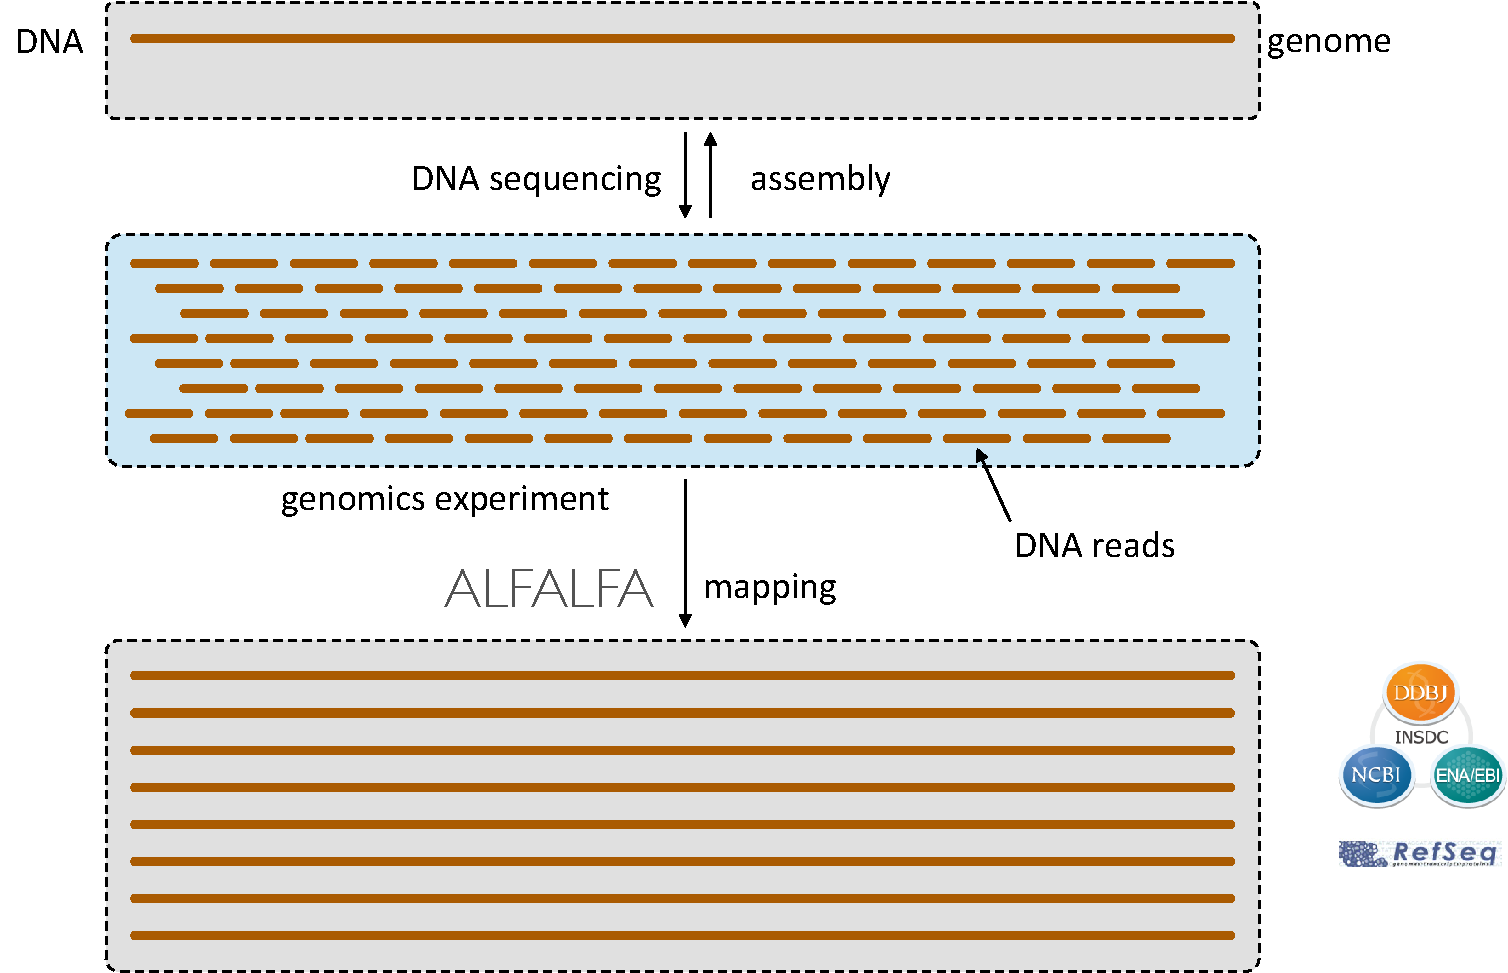
\includegraphics[width=0.8\textwidth]{includes/genomics}
	\caption{Illustratie van een genomics experiment. Een genoom, voorgesteld 
	door een bruine lijn, wordt gesequeneerd in verschillende DNA reads. Deze 
	reads kunnen dan opnieuw worden geassembleerd naar een volledig 
	consensusgenoom of kunnen worden gemapt op meerdere genomen aan de hand van 
	DNA read 
	mappers en genoomdatabanken.}
	\label{fig:genomics}
\end{figure}

Verwant aan het genoom is het proteoom. De studie van proteomen wordt proteomics
genoemd. Een proteoom bestaat uit de volledige set aan eiwitten die geëncodeerd
in door een genoom, een organisme of een deel ervan. Net als een genoom kan een
proteoom ook worden gesequeneerd in protein reads, peptiden genaamd. Die protein
reads kunnen dan net zoals DNA reads gemapt worden aan de hand van tools, zoals
Unipept\cites{mesuere2012unipept, mesuere2014unipept}, worden gemapt op
eiwitdatabanken, zoals geïllustreerd in \Vref{fig:proteomics}.
UniProt\cite{uniprot2014uniprot} is een voorbeeld van zo'n soort eiwitdatabank.

\begin{figure}
	\centering
	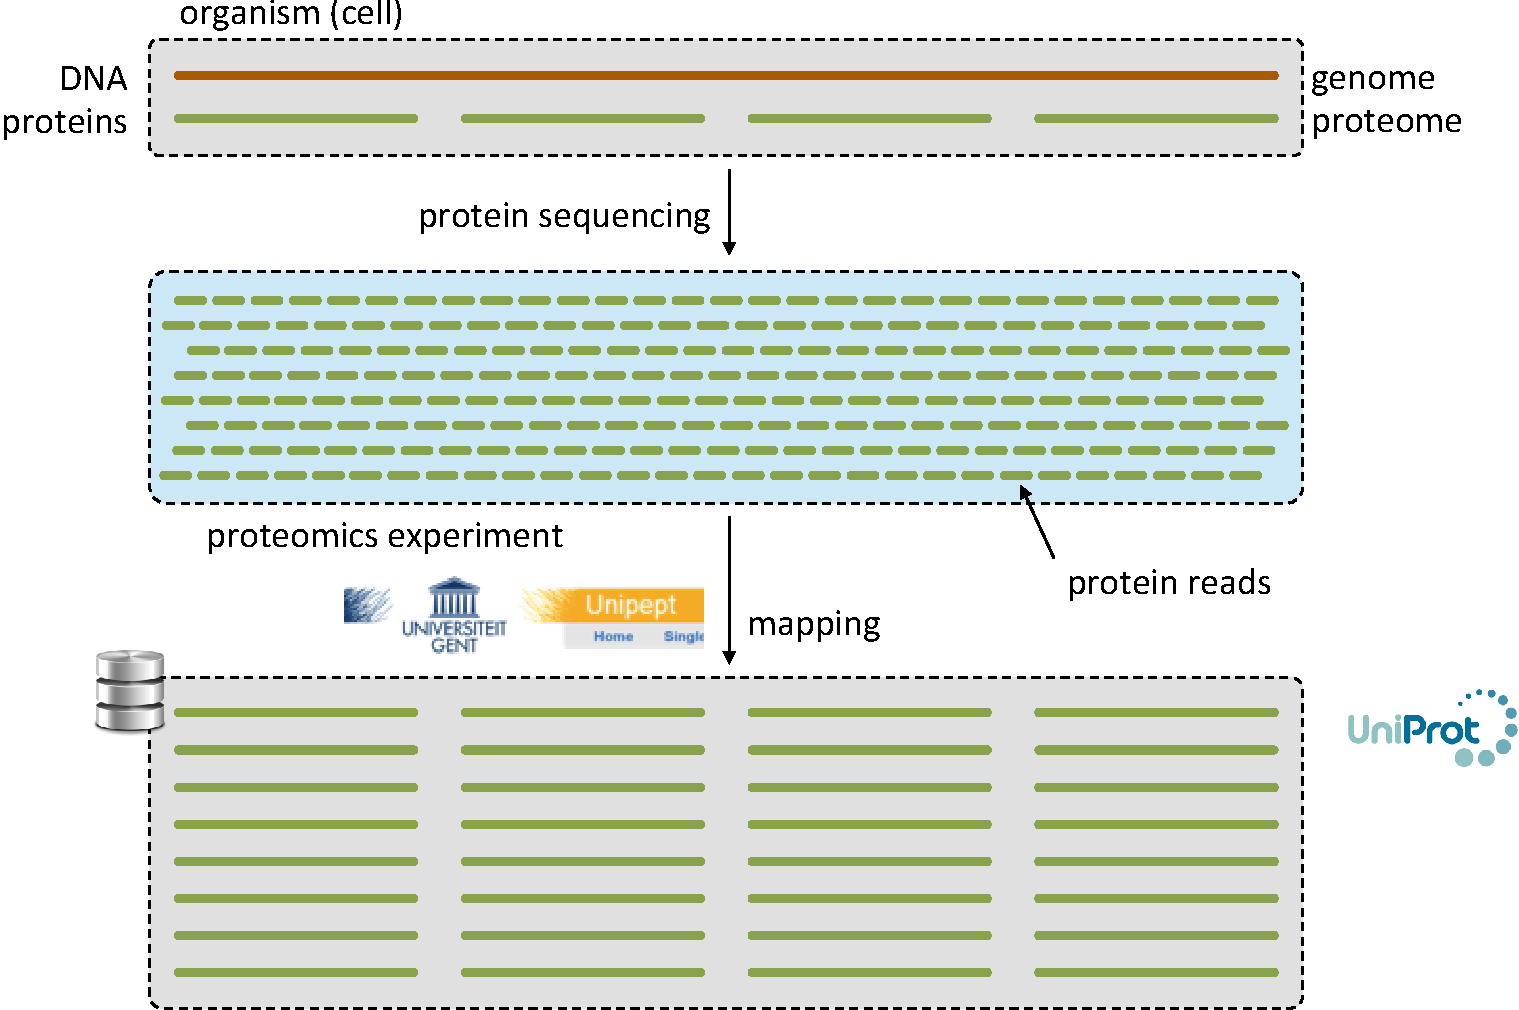
\includegraphics[width=0.8\textwidth]{includes/proteomics}
	\caption{Illustratie van een proteomics experiment. Eiwitten, geannoteerd 
	op een genoom, worden gesequeneerd in protein reads. Die reads kunnen dan 
	worden gemapt op overeenkomstige proteomen uit eiwitdatabanken.}
	\label{fig:proteomics}
\end{figure}

\section{Metagenomics en metaproteomics} 

Wanneer stalen worden genomen uit de natuur, bijvoorbeeld bij vijveronderzoek,
of in de medische wereld, bijvoorbeeld bij de analyse van iemands stoelgang,
krijgen onderzoekers te maken met gemeenschappen in plaats van geïsoleerde
specimen. Ze hebben met andere woorden te maken met stalen van meerdere genomes
of metagenomes en meerdere proteomes of metaproteomes. Daarbij komt ook nog eens
dat slechts één procent van de organismen die in de natuur wordt gevonden, in
een lab kan worden gekweekt. Het is dus belangrijk om rechtstreeks met stalen
uit de natuur te kunnen werken en voor een vlotte analyse van die stalen is het
noodzakelijk dat er technieken bestaan die meerdere genomen en proteomen
tegelijkertijd kunnen verwerken en analyseren. Wanneer we het hebben over het
analyseren van metagenomes en metaproteomes bevinden we ons respectievelijk in
het onderzoeksgebied van de metagenomics en de metaproteomics.

Bij dit soort onderzoek zijn er drie grote vragen: \textit{i)} Welke organismen
bevinden zich in een staal? \textit{ii)} Wat doen ze precies? en \textit{iii)}
Hoe doen ze het? In deze thesis houden we ons vooral bezig met de eerste vraag.

Onderzoek in metagenomics gebeurt typisch op twee manieren. De eerste manier is
\emph{targeted metagenomics} waarbij een specifiek stuk, meestal een deel van
het 16S ribosomaal RNA, uit de verschillende organismen in het staal worden
gesequeneerd. Een tweede manier is \emph{shotgun metagenomics} waarbij de
volledige DNA strands uit het metagenoom worden gesequeneerd. Opnieuw aan de
hand van verschillende genoomdatabanken kan de mapping van die reads naar
gesequeneerde genomen gebeuren. Beide aanpakken zijn geïllustreerd in
\Vref{fig:metagenomics}.

\begin{figure}
	\centering
	\begin{subfigure}{0.49\textwidth}
		\centering
		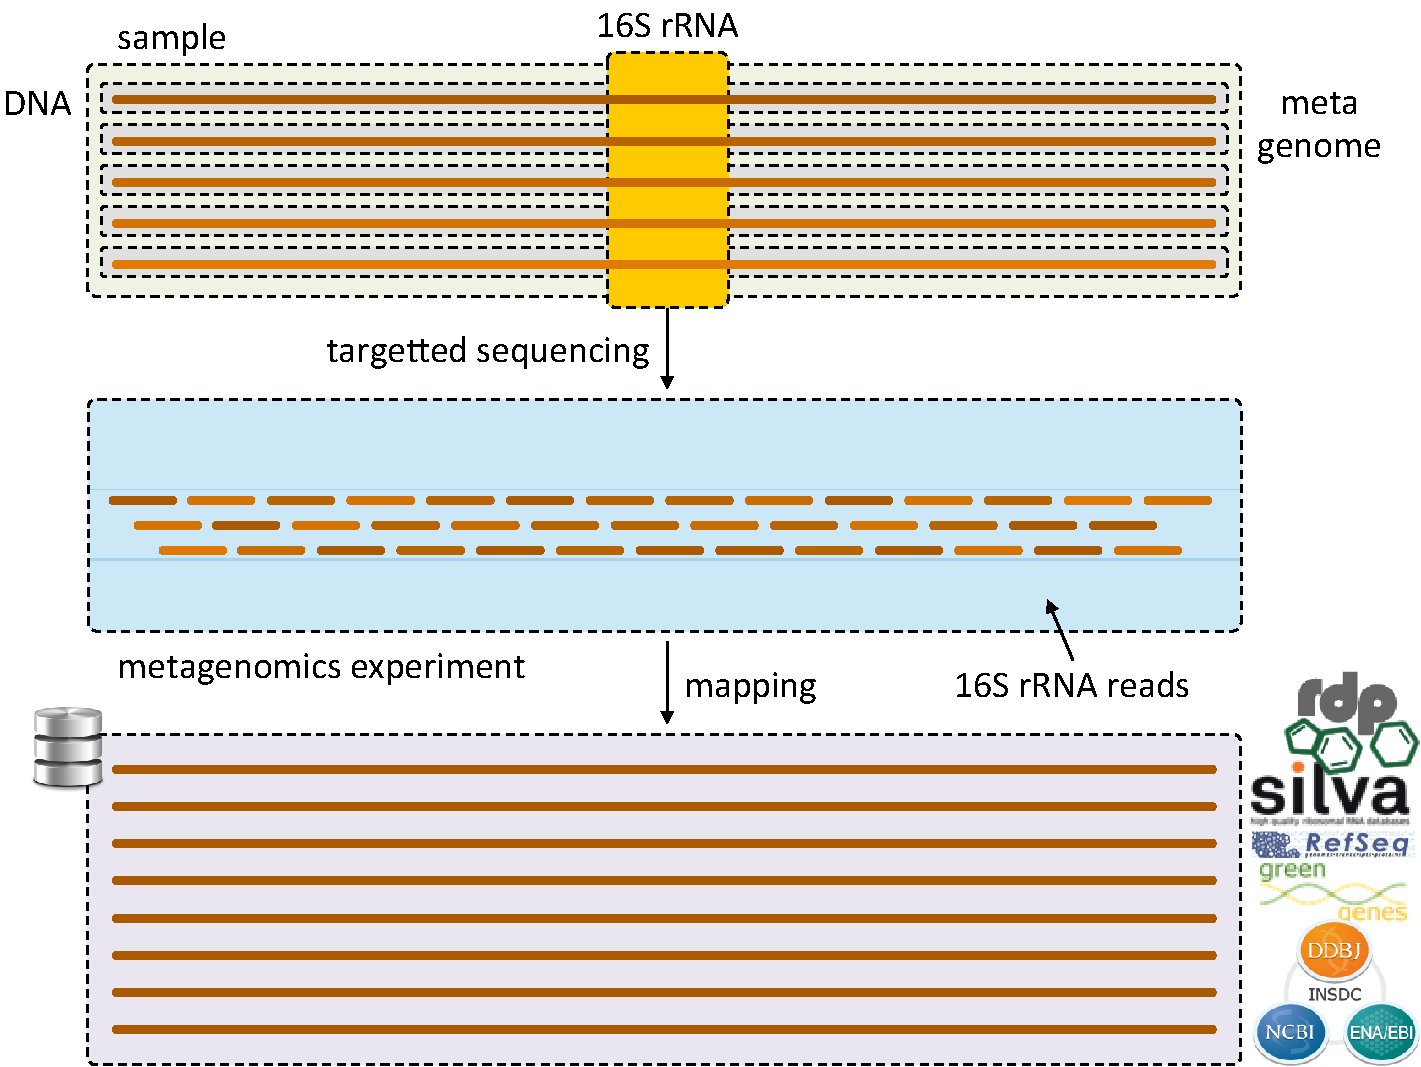
\includegraphics[width=\textwidth]{includes/targetted_metagenomics}
		\caption{}
	\end{subfigure}
	\begin{subfigure}{0.49\textwidth}
		\centering
		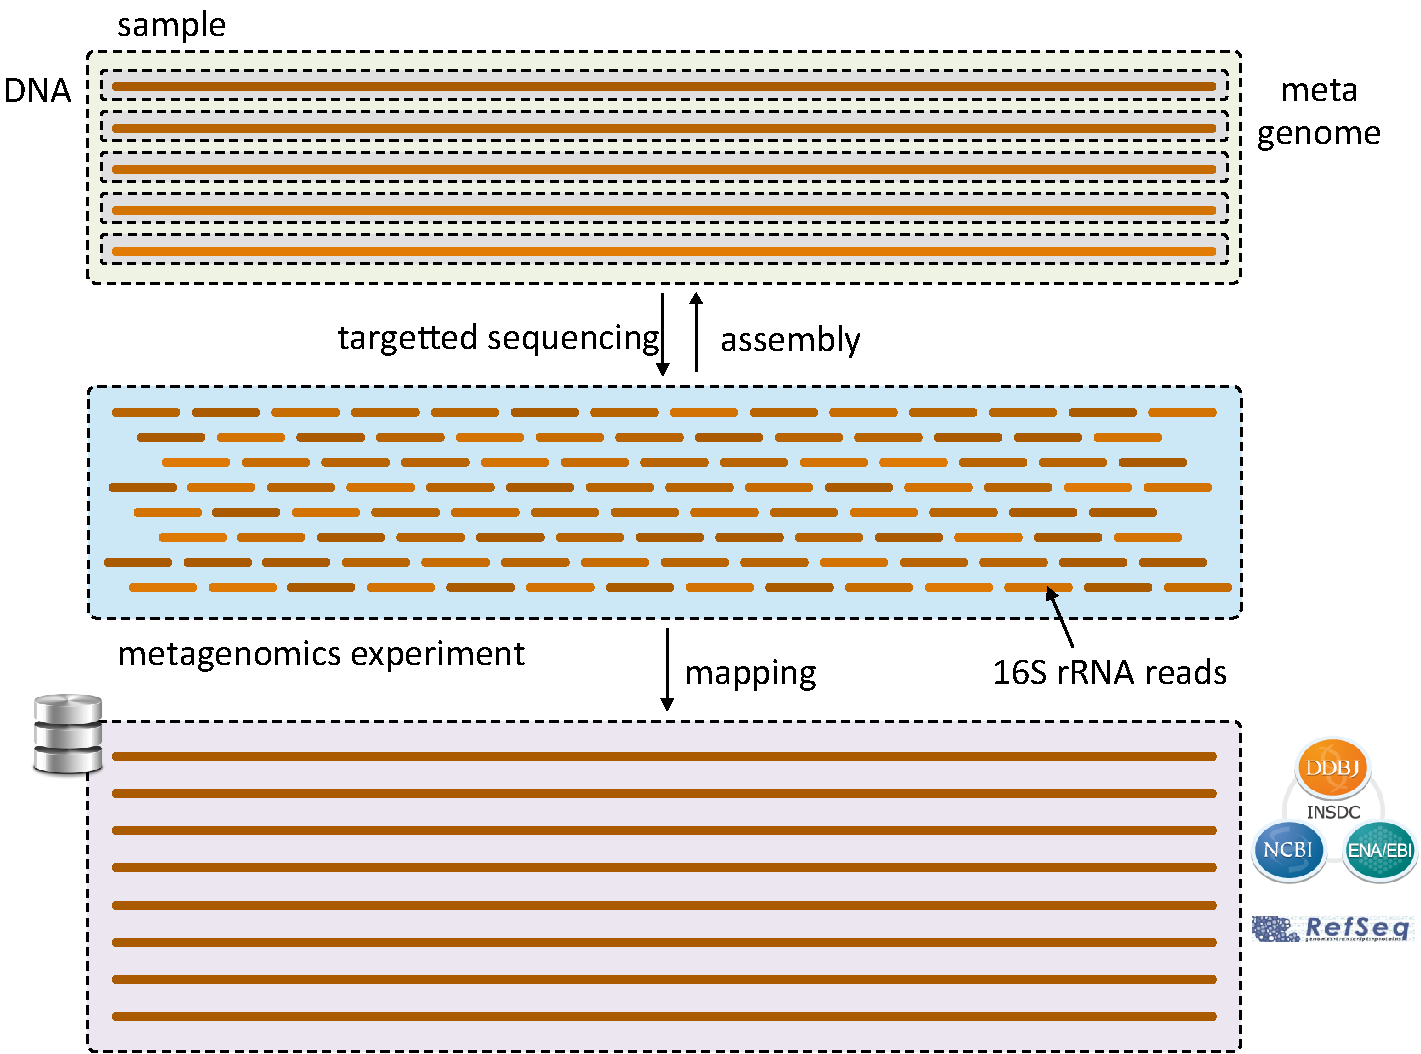
\includegraphics[width=\textwidth]{includes/shotgun_metagenomics}
		\caption{}
	\end{subfigure}
	
	\caption{Illustratie van een metagenomics experiment. Links de 16S rRNA 
	variant, rechts de shotgun variant. Bij een metagenomics experiment wordt 
	(een gedeelte van) de DNA strands uit een metagenoom gesequeneerd en daarna 
	op genoomdatabanken gemapt.}
	\label{fig:metagenomics}
\end{figure}

Het proces van metagenomics kan, analoog aan de processen van genomics en 
proteomics, toegepast worden op metaproteomics. Dat wordt geïllustreerd in 
\Vref{fig:metaproteomics}. Hierbij worden alle eiwitten op de DNA strands uit 
het sample geannoteerd en gesequeneerd in protein reads of peptiden. Die 
peptiden kunnen vervolgens opnieuw, bijvoorbeeld door Unipept, worden gemapt op 
eiwitdatabanken.

\begin{figure}
	\centering 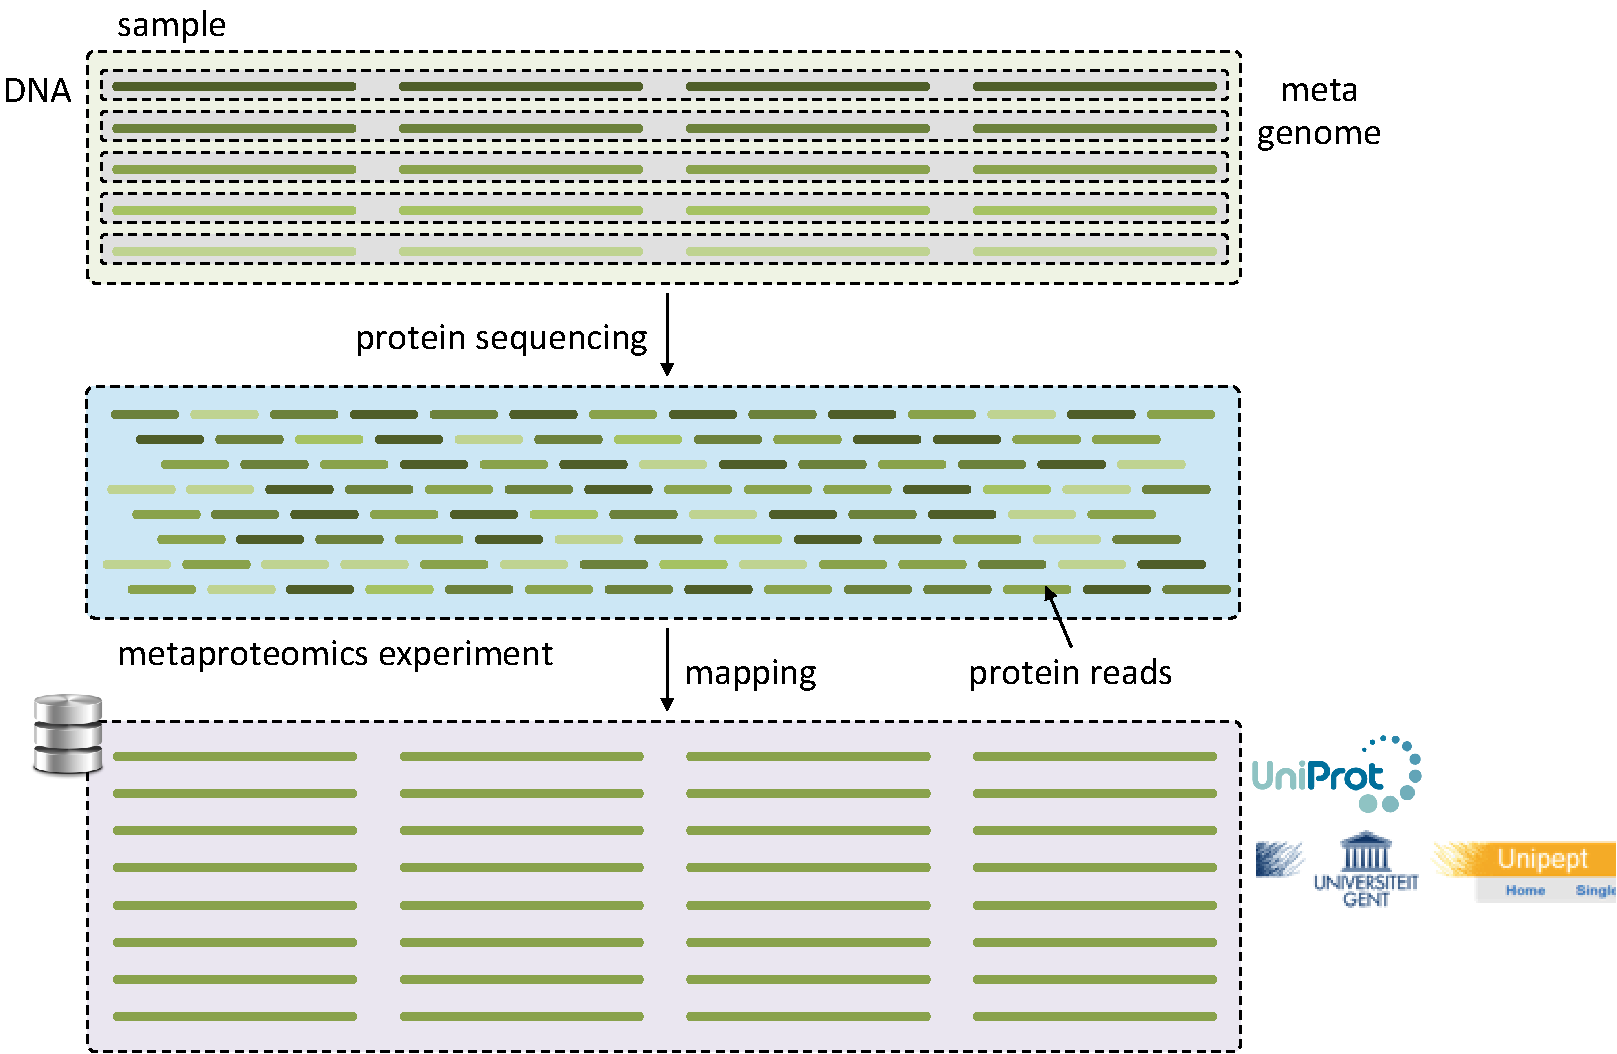
\includegraphics[width=0.8\textwidth]{includes/metaproteomics}
	\caption{Illustratie van een metaproteomics experiment. Alle eiwitten,
	geannoteerd op de verschillende DNA strands, worden gesequeneerd in
	protein reads, peptiden genaamd. Die peptiden kunnen dan worden gemapt op
	overeenkomstige proteomen aan de hand van eiwitdatabanken.}
	\label{fig:metaproteomics}
\end{figure}

\section{Van metagenoom naar metaproteoom}
De klassieke oplossing voor de mapping van een reeks DNA reads op genomen in een
genoomdatabank is het gebruik van BLAST, of verwante tools. Die tools zijn vaak
zeer traag en vereisen zeer veel rekencapaciteit.  Aangezien Unipept
al in staat is om zeer snel metaproteomen te analyseren zou het erg voordelig
zijn om dat metagenomics probleem om te zetten naar een metaproteomics probleem.
Dat is dan ook wat we proberen te doen. Het grootste voordeel van die omzetting
is dat we voor de meeste stappen integraal gebruik kunnen maken van de Unipept
Metaproteomics Analyse Pipeline. Die pipeline is al geïmplementeerd en 
geoptimaliseerd om alles in zo weinig mogelijk tijd te berekenen. Wat dan 
nog rest is de conversie van en naar metagenomics.

De omzetting zelf gebeurt volgens de werkwijze aangegeven in
\Vref{fig:van_naar}. Voor elke DNA read in een metagenomics dataset kunnen we
een proteomics experiment doen. Hierbij zoeken we, bijvoorbeeld aan de hand van
FragGeneScan, alle (fragmenten van) eiwitten in de DNA read in kwestie. De
bekomen eiwitten worden opgedeeld in tryptische peptiden, waarna elke peptide
afzonderlijk op zijn taxonomische identificatie wordt gemapped door middel van
het lowest common ancenstor (LCA) algoritme. Aan de hand van een uitbreiding van
dit lowest common ancestor algoritme kunnen we de bekomen taxa aggregeren naar
een consensusclassificatie. Dat proces zullen we vanaf nu aanduiden met de
Unipept Metagenomics Analysis Pipeline, of ook wel UMAP.

\begin{figure}[hbt]
	\centering 
	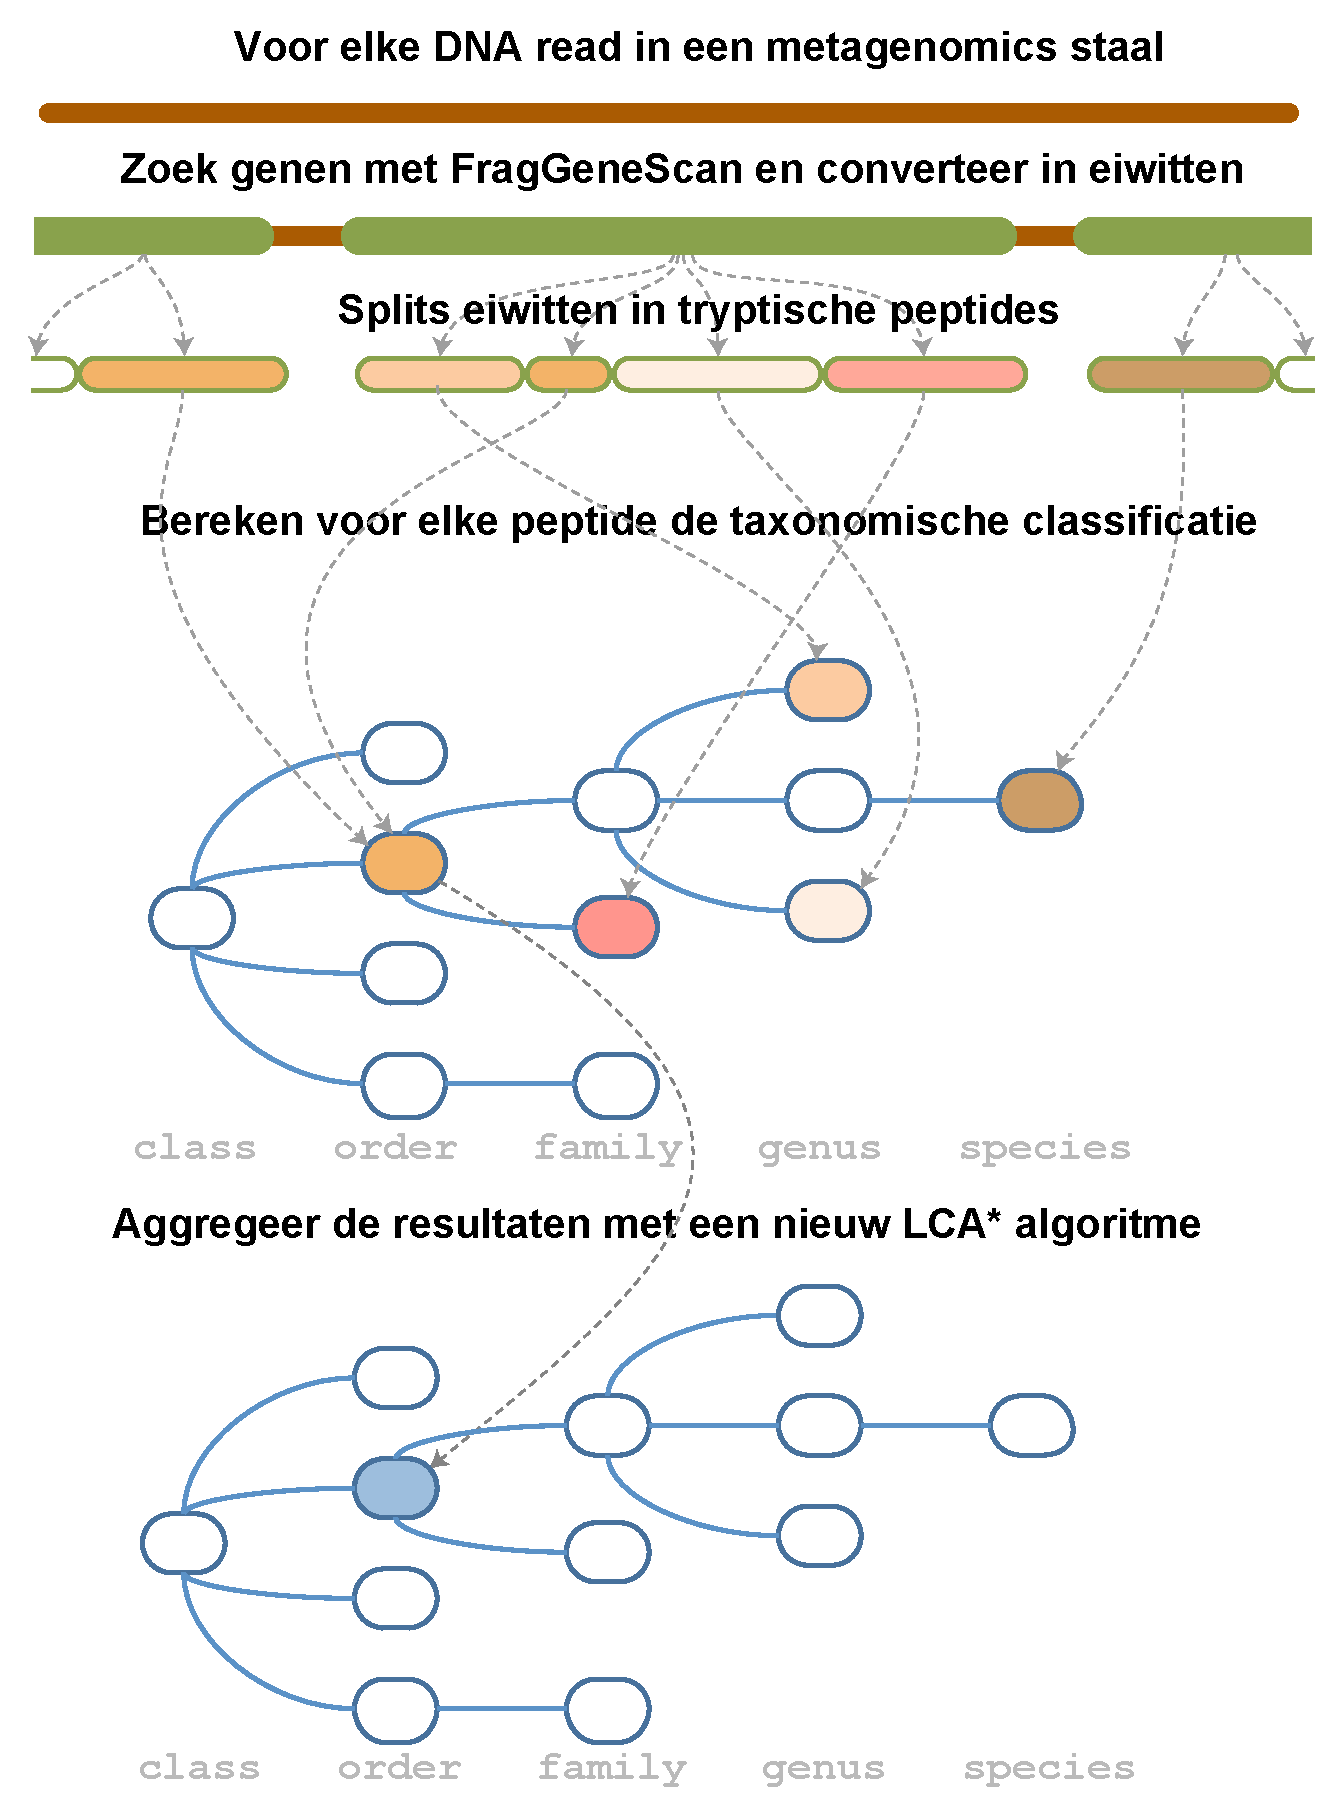
\includegraphics[width=0.6\textwidth]{includes/van_metagenoom_naar_metaproteoom}
	\caption{Illustratie van de werkwijze om een metagenomics probleem om te 
	zetten naar een metaproteomics probleem. Voor elke DNA read in het 
	metagenomics sample kunnen we een proteomics experiment doen. Hierbij 
	zoeken we, bijvoorbeeld aan de hand van FragGeneScan, alle eiwitten op 
	de DNA read in kwestie. De bekomen eiwitten worden opgedeeld in 
	tryptische peptiden waarna elke peptide afzonderlijk op zijn taxonomische 
	identificatie wordt gemapped door middel van het lowest common ancestor 
	(LCA) algoritme. Aan de hand van een uitbreiding van dit lowest common 
	ancestor algoritme kunnen we de bekomen taxa aggregeren naar een 
	consensusclassificatie.}
	\label{fig:van_naar}
\end{figure}

In \Vref{chap:lca*} bespreken we de motivatie en implementatie van het nieuwe 
LCA* algoritme gebruikt in de laatste stap, waarna we in \Vref{chap:casestudy} 
de performantie benchmarken van de nieuwe Unipept Metagenomics Analysis 
Pipeline.

\section{Unipept}
In dit hoofdstuk is de naam Unipept een aantal keer gevallen. Aangezien deze
thesis kadert binnen het Unipept-project wordt in deze sectie een korte
beschrijving van Unipept gegeven en wordt uitgelegd waar Unipept zich momenteel
bevindt in de bovenstaande processen.

Kort samengevat is Unipept een framework met een gebruiksvriendelijke
webinterface om de biodiversiteit van grote en complexe metaproteomics samples
te onderzoeken aan de hand van informatie uit tryptische peptiden. Achter de
webinterface bevindt zich een indexstructuur die ervoor gemaakt is om snel alle
eiwitten uit de UniProtKB op te vragen waar de tryptische peptide in voorkomt.
Door het gebruik van een speciale lowest common ancestor aanpak kan ook de
taxonomische identificatie aan een peptide gekoppeld worden die bestand is tegen
verkeerde identificaties, classificaties en onjuistheden in de taxonomieboom.
Die achterliggende indexstructuur is naast de webinterface ook aanspreekbaar
via de Unipept command-line interface (CLI) die een interface aanbiedt voor de 
Unipept web services. De CLI laat de gebruiker toe grote datasets te verwerken 
zonder dat via de browser te moeten doen.

\Vref{chap:cli} geeft na een inleiding tot de Unipept command-line interface een
reeks van problemen met bijhorende oplossingen die naar boven zijn gekomen
tijdens het intensief gebruik van de tools. In \Vref{chap:vis} geven we een
overzicht van de al bestaande visualisaties in Unipept. Daarnaast motiveren we
de abstractie en modularisatie van die visualisaties in een apart Unipept
visualisation framework.

\section{Geschreven code}

Alle code geschreven binnen de context van deze thesis is verzameld op de UGent
GitHub onder de Unipept organisatie en voornamelijk onder de repositories
\texttt{unipept-visualizations} en \texttt{unipept-metagenomics-scripts}.
Toegang tot deze repositories kan gegeven worden door de promotor of begeleider
van deze thesis.
\chapter{LCA*}
\label{chap:lca*}

In dit hoofdstuk leggen we eerst het algemene concept van de lowest common
ancestor (LCA) uit. We bekijken de verschillende toepassingen van dit concept in
de biologie en lichten toe hoe dit LCA algoritme wordt gebruikt in
Unipept. Na deze inleiding stellen we een variant van dat algoritme voor,
LCA*, en leggen we uit waarom LCA* in sommige gevallen een specifieker
resultaat oplevert dan algemene LCA. Hierna diepen we een zeer snelle
implementatie van het originele LCA algoritme uit, tonen we aan hoe we dit
algoritme kunnen uitbreiden tot een algoritme voor LCA* en lossen we enkele 
problemen op die die uitbreiding met zich meebrengt. We sluiten af met een
voorbeeld van hoe LCA* zou kunnen worden ingebouwd in de Unipept webservices.

\section{Inleiding}
Het lowest common ancestor (LCA) probleem is een klassiek probleem in de
grafentheorie. De LCA in een boomstructuur wordt gedefinieerd als de
gemeenschappelijke ouder van twee (of meer) nodes die zich het verst van de
wortel bevindt. Toegepast op het voorbeeld in \Vref{tikz:lcavoorbeeld}, kunnen
we bijvoorbeeld de LCA berekenen van node E en J. Nodes waarvan we de LCA
berekenen, zullen we in het vervolg ``querynodes'' noemen. Volgens de definitie
hierboven is de LCA van E en J gelijk aan C. De notatie die we hier in het
vervolg voor zullen gebruiken is: LCA(E, J) = C. Wanneer we de LCA berekenen van
twee nodes op hetzelfde pad, resulteert dit in de node dichtst bij de wortel,
zoals te zien is op \Vref{tikz:lcadg}.

\begin{figure}
    \centering
    
    \begin{subfigure}{0.45\linewidth}
        \centering
        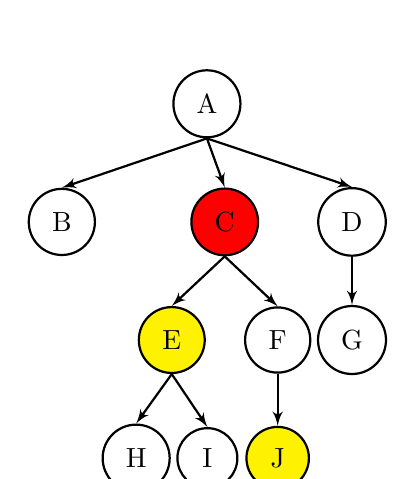
\begin{tikzpicture}[node distance=3cm, level distance=1.5cm,
            every node/.style={draw, thick, circle,inner sep=5pt},
            every path/.style={->, draw, thick, -latex'}]
        \Tree [. A 
                 [. B ]
                 [. \node[draw, fill=red]{C};
                    [.\node[draw, fill=yellow]{E};
                       [. H ]
                       [. I ]
                    ]
                    [. F
                       [. \node[draw, fill=yellow]{J}; ]
                    ] 
                 ]
                 [. D
                    [ . G ]
                 ] 
              ]
        \end{tikzpicture}
        \caption{}
        \label{tikz:lcaej}
    \end{subfigure}
    \begin{subfigure}{0.45\linewidth}
        \centering
        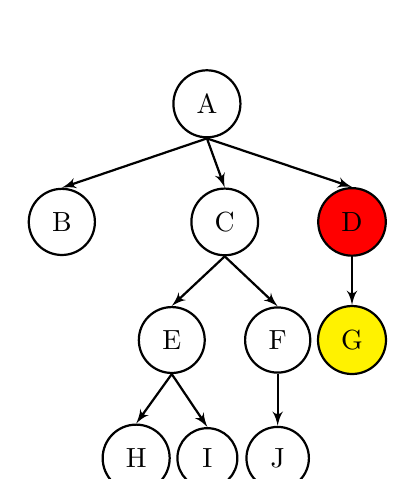
\begin{tikzpicture}[node distance=3cm, level distance=1.5cm,
            every node/.style={draw, thick, circle,inner sep=5pt},
            every path/.style={->, draw, thick, -latex'}]
        \Tree [. A 
                 [. B ]
                 [. C
                    [. E
                       [. H ]
                       [. I ]
                    ]
                    [. F
                       [. J ]
                    ] 
                 ]
                 [. \node[draw, fill=red]{D};
                    [ . \node[draw, fill=yellow]{G}; ]
                 ] 
              ]
        \end{tikzpicture}
        \caption{}
        \label{tikz:lcadg}
    \end{subfigure}
                
    \caption{Bovenstaande figuren worden twee voorbeelden getoond van het
    algemene LCA concept. Links nemen we de LCA van node E en J, met C als
    resultaat. Rechts berekenen we de LCA van twee nodes op hetzelfde pad, D en
    G. Dit geeft de node dichtst bij de wortel als resultaat, namelijk D. Nodes
    in het geel zijn de nodes waarvan de LCA wordt berekend, de rode nodes zijn
    het resultaat van de LCA bewerking.} 
    \label{tikz:lcavoorbeeld}
\end{figure}

Binnen de (meta)proteomics wordt de berekening van de LCA ook vaak gebruikt. Dit
wordt geïllustreerd in \Vref{fig:workflow} waar in de laatste stap de LCA
genomen wordt van alle gevonden taxa in de Unipept taxonomy.

\begin{figure}
	\centering
    \includegraphics[width=0.8\textwidth]{includes/workflow}
    \caption{Illustratie van het gebruik van lowest common ancestor binnen de 
    (meta)proteomics. Het lowest common ancestor algoritme wordt hier gebruikt 
    om in de laatste stap de gevonden taxa in de Unipept taxonomie te 
    aggregeren tot één consensustaxon.}
    \label{fig:workflow}
\end{figure}

De metagenomics toolchain, geïllustreerd in \Vref{fig:van_naar}, voert op het
resultaat van de LCA nogmaals een LCA stap uit waarbij alle gevonden taxa
geaggregeerd worden tot één consensustaxon. Het toepassen van het LCA algoritme
zoals hierboven beschreven levert echter niet altijd het gewenste resultaat op.
Onderstaand voorbeeld illustreert waarom.

Stel dat we in een tropisch oerwoud een onbekende plant tegenkomen en willen
weten welke (soort) plant dit is, dan kunnen we een experiment doen. We nemen
van deze plant een sample en verwerken het via de technieken beschreven in de
inleiding, zodat we uiteindelijk een reeks van peptiden bekomen. Voor elke
peptide uit deze reeks kunnen we dan alle taxa opzoeken waar de peptiden in
voorkomen. Stel nu dat dit resulteert in volgende resultaat: 95\% van de taxa
behoort tot het rijk (\textit{kingdom}) van de groene planten, de Viridiplantae
en voor 5\% behoort tot het geslacht (\textit{genus}) van de bananenplanten, de
Musa. We kunnen dan beide groepen als verzamelingen voorstellen: de planten =
\{baardgras, distel, banaan, maanvaren, ...\}. De verzameling van de
bananenplanten wordt dan: \{\textit{callimusa}, \textit{ingentimusa}, ...\}. De
bananenplanten zijn dus een deelverzameling van alle planten. Een visuele
representatie van dit voorbeeld is te vinden in \Vref{tikz:verzameling}.

\begin{figure}
	\centering
    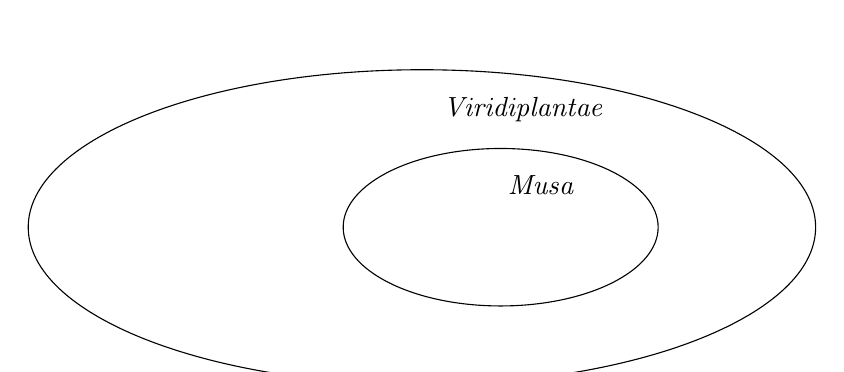
\begin{tikzpicture}
        \draw (0,0) ellipse (5 and 2);
        \node at ($(0,0)+(75:5 and 1.55)$) {\textit{Viridiplantae}};
        \draw (1,0) ellipse (2 and 1);
        \node at ($(1,0)+(75:2 and 0.55)$) {\textit{Musa}};
    \end{tikzpicture}
    \caption{Illustratie van de verzameling van de \textit{Viridiplantae} en de 
    \textit{Musa}}
    \label{tikz:verzameling}
\end{figure}


Wanneer beide verzamelingen op een boomstructuur worden weergeven, zou dit
opnieuw voorgesteld kunnen worden zoals op \cref{tikz:lcadg}, waarbij D de
klasse van alle planten voorstelt en G die van de bananen.

Als het LCA algoritme wordt uitgevoerd op deze twee nodes zouden we als
resultaat op node D, de planten, uitkomen. Ook al is dit correct, is er toch een
specifiekere identificatie mogelijk. We weten namelijk dat alle peptiden uit de
sample die we in oerwoud hebben genomen uit één enkele plant afkomstig zijn.

Tijdens ons onderzoek hebben we gevonden dat er 5\% van de peptiden enkel en
alleen voorkomen bij bananenplanten. Het zou zonde zijn dit bewijs zomaar te
negeren en te besluiten dat de onderzochte plant tot het rijk (\textit{kingdom})
van de planten behoort, terwijl we ook specifiekere informatie kunnen geven;
namelijk dat de onderzochte plant tot de klasse van de bananenplanten behoort.
Aangezien er peptiden van de bananenplant in het sample voorkomen, kunnen we
daar namelijk uit afleiden dat we specifiek met een bananenplant te maken
hebben, en niet algemeen met een plant.

Als we terugkeren naar onze verzamelingen in \Vref{tikz:verzameling}, willen we
nu niet de unie nemen van beide verzamelingen. Dat zou immers de minder
specifieke klasse van de planten opleveren. Wat we willen, is de specifiekere
identificatie van de plantensoort (namelijk de bananenplant) en dat bekomen we
door de doorsnede van beide verzamelingen te nemen.

Wanneer de doorsnede van beide verzamelingen leeg is, is er geen specifiekere
identificatie mogelijk en nemen we alsnog de unie, zoals in \cref{tikz:lca*ej}
wordt geïllustreerd.

Deze variant van de LCA zullen we om verwarring te vermijden, aanduiden met
LCA*.

\begin{figure}
    \centering
    
    \begin{subfigure}{0.45\linewidth}
        \centering
        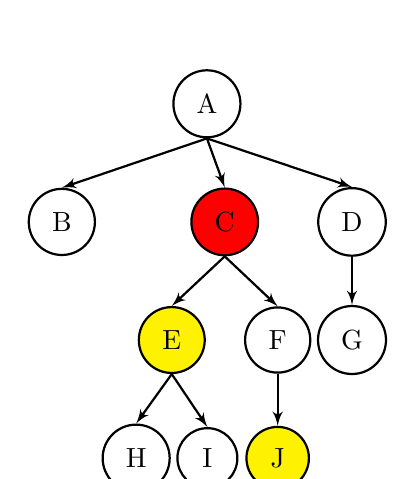
\begin{tikzpicture}[node distance=3cm, level distance=1.5cm,
            every node/.style={draw, thick, circle,inner sep=5pt},
            every path/.style={->, draw, thick, -latex'}]
        \Tree [. A 
                 [. B ]
                 [. \node[draw, fill=red]{C};
                    [.\node[draw, fill=yellow]{E};
                       [. H ]
                       [. I ]
                    ]
                    [. F
                       [. \node[draw, fill=yellow]{J}; ]
                    ] 
                 ]
                 [. D
                    [ . G ]
                 ] 
              ]
        \end{tikzpicture}
        \caption{}
        \label{tikz:lca*ej}
    \end{subfigure}
    \begin{subfigure}{0.45\linewidth}
        \centering
        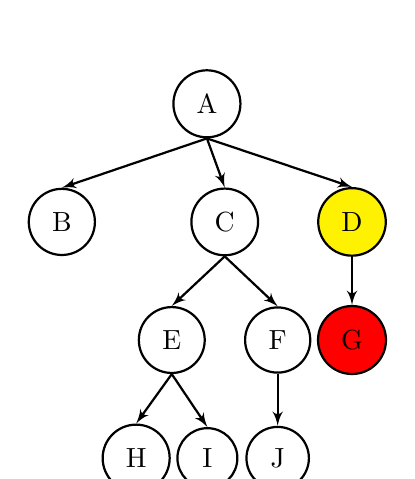
\begin{tikzpicture}[node distance=3cm, level distance=1.5cm,
            every node/.style={draw, thick, circle,inner sep=5pt},
            every path/.style={->, draw, thick, -latex'}]
        \Tree [. A 
                 [. B ]
                 [. C
                    [. E
                       [. H ]
                       [. I ]
                    ]
                    [. F
                       [. J ]
                    ] 
                 ]
                 [. \node[draw, fill=yellow]{D};
                    [ . \node[draw, fill=red]{G}; ]
                 ] 
              ]
        \end{tikzpicture}
        \caption{}
        \label{tikz:lca*dg}
    \end{subfigure}
                
    \caption{Voorbeelden van het LCA* algoritme. Links wordt LCA*(E, J) = C 
    uitgewerkt, rechts
    LCA*(D, G) = G. Nodes in het geel zijn de nodes waarvan de LCA wordt
    berekend, de rode nodes zijn de resulterende LCA*.}
    \label{tikz:lca*voorbeeld}
\end{figure} 

\section{Huidige implementatie in Unipept} 

Zoals geïllustreerd wordt in \Vref{fig:workflow} worden uit de UniProtKB alle
eiwitten opgezocht waar een gegeven peptide in gevonden wordt. Voor die lijst
van eiwitten wordt hun overeenkomstig taxon uit de NCBI taxonomie opgezocht.
Die taxa worden dan afgebeeld op de Unipept taxonomie, die een opgekuiste versie
is van de NCBI taxonomie. Onder andere uncultured, unspecified, mixed, ...
culturen zijn weggefilterd in de Unipept taxonomie. Nu wordt de resulterende
lijst van taxa in de Unipept taxonomie geaggregeerd tot één consensustaxon voor
het originele peptide via de LCA methode. In deze sectie bespreken we de huidige
implementatie van deze methode en welke beperkingen die met zich meebrengt.

\subsection{Tabelgebaseerde LCA}
De implementatie van de LCA in Unipept is het eenvoudigst te begrijpen aan de 
hand van een voorbeeld. In \Vref{tbl:tabelvoorbeeld} worden alle gevonden taxa 
waar de peptide \texttt{MFNWMVTR} in voorkomt opgelijst, met daarnaast hun 
lineage naar de root. Om de LCA te vinden van deze wordt de tabel van links 
naar rechts overlopen, startend bij de minst specifieke rang. In het voorbeeld 
is dit dus de rang \textit{superkingdom}. Aangezien alle organismes zich 
binnen hetzelfde superkingdom bevinden, namelijk de Eukaryota, schuiven we een 
rang op naar rechts. Ook bij de rang \textit{kingdom} zien we dat alle 
organismes zich binnen hetzelfde kingdom bevinden. Op deze manier schuiven we 
steeds naar rechts -- dus naar een specifiekere rang op -- tot we bij de rang 
\texttt{class} komen. Tot op dit niveau is het eerste organisme niet 
gespecifieerd en verschillen ook de groepen van de overige peptides. Peptide 2 
tot en met 5 bevinden zich binnen de rang van de \textit{Aves} en die daarna 
bevinden zich binnen de rang van de \textit{Mammalia}. Dit is dus een 
splitsing van de takken in de taxonomie en nemen we de vorige rang als LCA 
resultaat. In het voorbeeld is dat dus de \textit{Craniata} binnen de rang 
\textit{subphylum}.

\section{Beperkingen van de tabelmethode}
De huidige implementatie in Unipept met de tabelgebaseerde methode is zeer snel
aangezien alle mogelijke LCAs kunnen worden voorberekend, maar kent wel enkele
beperkingen. In de NCBI taxonomy zijn er een heel aantal organismen aanwezig die
niet geclassificeerd zijn onder een rang zoals rijk, familie, genus, etc. Deze
organismen worden wel in de taxonomie opgenomen waar ze als rangloos
geclassificeerd worden.

In \Vref{tbl:tabelvoorbeeld} zien we het ingekorte resultaat van de tryptische
peptide analyse op de peptide \texttt{MFNWMVTR}. Als LCA wordt hiervoor door
Unipept het subphylum \textit{Craniata} gevonden. Wanneer we echter de
\textit{Craniata}, de \textit{Aves} en de \textit{Mammalia} op een boomstructuur
visualiseren krijgen we het resultaat uit \Vref{fig:boomvoorbeeld}. Als we 
op de boom de LCA zoeken van de Mammalia en de Aves komen we uit bij de Amniota,
en niet bij de Craniata. De tiental onderverdelingen tussen de Craniata en de
Amniota zijn allemaal rangloos.

We zien dus dat er door het omzetten van de boom in een tabulaire voorstelling
(waarin enkel de ranghebbende taxa worden voorgesteld) veel informatie verloren
gaat. Een stap naar specifiekere classificaties is dus om een nieuwe methode te
implementeren die rechtstreeks op de boom werkt en zo ook rekening houdt met
tussenliggende rangloze taxa.

\begin{table}
	\centering
	
	\caption{(Ingekorte) tryptische peptide analyse van peptide 
	\texttt{MFNWMVTR}}
	\label{tbl:tabelvoorbeeld}
	\scriptsize
	\begin{tabular}{llllllll}
        \toprule
        Organism & Superkingdom & Kingdom & Phylum & Subphylum & Class & 
        Superorder & ... \\
        \midrule
        Pelodiscus sinensis & Eukaryota & Metazoa & Chordata & Craniata &  &  & 
        ... \\
        Columba livia & Eukaryota & Metazoa & Chordata & Craniata & Aves & 
        Neognathae & ... \\
        Meleagris gallopavo & Eukaryota & Metazoa & Chordata & Craniata & Aves 
        & Neognathae & ... \\
        Ficedula albicollis & Eukaryota & Metazoa & Chordata & Craniata & Aves 
        & Neognathae & ... \\
        Taeniopygia guttata & Eukaryota & Metazoa & Chordata & Craniata & Aves 
        & Neognathae & ... \\
        Ornithorhynchus anatinus & Eukaryota & Metazoa & Chordata & Craniata & 
        Mammalia &  & ... \\
        Monodelphis domestica & Eukaryota & Metazoa & Chordata & Craniata & 
        Mammalia &  & ... \\
        Sarcophilus harrisii & Eukaryota & Metazoa & Chordata & Craniata & 
        Mammalia &  & ... \\
        ... & ... & ... & ... & ... & ... & ... & ... \\
        \bottomrule
	\end{tabular}
\end{table}

\begin{figure}
    \centering
    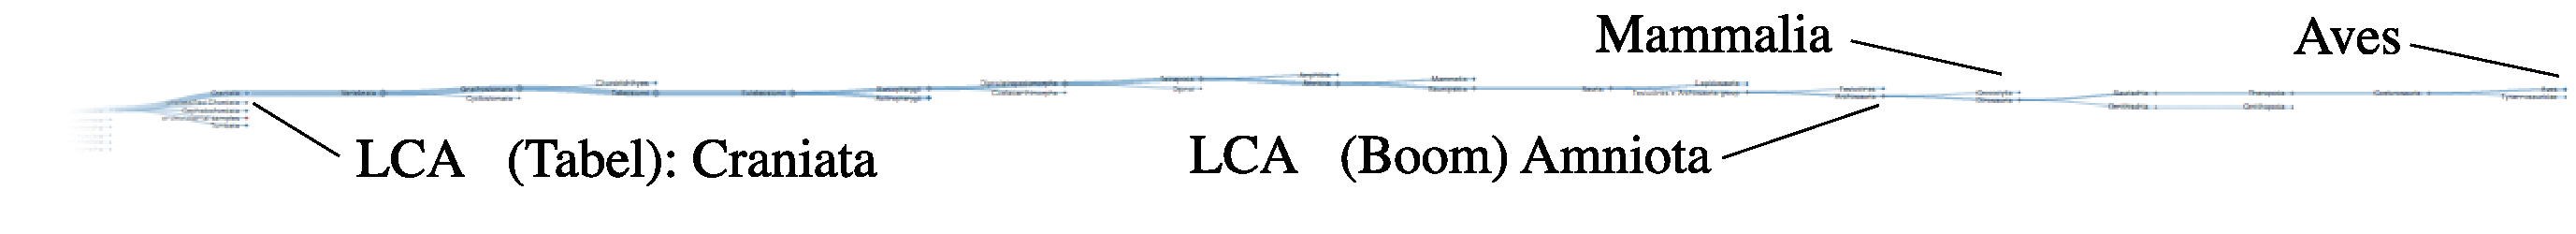
\includegraphics[width=1\textwidth]{includes/tabelanalyse}
    \caption{Weergave van \textit{Mammalia} en \textit{Aves} op de tak van de
    \textit{Craniata}. We zien dat de LCA op de tabel resulteert in
    \textit{Craniata}, terwijl de boomgebaseerde LCA de \textit{Amniota} vindt.
    Tussen de \textit{Craniata} en de \textit{Amniota} staan echter een tiental
    rangloze organismen. De boomgebaseerde taxonomische identificatie is dus een
    stuk specifieker.}
    \label{fig:boomvoorbeeld}
\end{figure}

\section{Boomgebaseerde LCA(*)} De hierboven genoemde reden is niet de enige
waarom het wenselijk is om een boomgebaseerde implementatie te maken. Zoals in
\Vref{chap:inleiding} beschreven is de laatste stap in de analyse om individuele
identificaties van alle peptiden uit een eiwit(fragment) of DNA read tot één
consensus te aggregeren.

In deze sectie diepen we het LCA* algoritme verder uit. We starten met een
implementatiebespreking van het gewone LCA algoritme en breiden die uit naar een
algoritme voor LCA*. Daarna bespreken we enkele problemen die voorkomen bij de
omvorming en hun oplossingen.

De berekening moet natuurlijk zo snel mogelijk verlopen. Daarom zouden we
dezelfde aanpak kunnen toepassen als Unipept om de LCA's van alle peptiden voor
te berekenen. Op die manier zouden we alle resultaten in een databank kunnen
opslaan, zodat we ze er in constante tijd uit kunnen halen. Die oplossing is
helaas onmogelijk door het gigantische aantal mogelijke combinaties van taxa die
als invoer kunnen worden gegeven. Er zijn op het moment van schrijven 1.267.511
taxa aanwezig in de NCBI taxonomy. Alle mogelijke subsets uit deze verzameling
voorberekenen zou onmogelijk zijn. Bij het voorberekenen van de LCAs van alle
peptiden (1.713.298.862) is dat wel mogelijk met voldoende opslagcapaciteit.

Iets wat we eventueel wel kunnen uitbuiten is de datastructuur waarop alle
analyses zullen uitgevoerd worden. Die is namelijk altijd dezelfde.

\subsection{Implementatie}
In deze sectie bespreken we een algoritme om de LCA van een opgegeven lijst van
nodes in een boomstructuur te berekenen. We tonen de tijd- en
ruimtecomplexiteiten van deze implementatie aan en bespreken vervolgens hoe we
het algoritme kunnen uitbreiden om als algoritme voor LCA* te gebruiken.

\subsubsection{State of the art}

Om het LCA probleem op te lossen, kijken we eerst naar de state of the art van
dit probleem. We baseren ons op het artikel ``Lowest Common Ancestors in Trees
and Directed Acyclic Graphs'' van Michael A. Bender en Martin Farach-Colton
\cites{lcabenderfarach}. In het artikel wordt een algoritme beschreven om het
LCA probleem in lineaire tijd te preprocessen. Dat kan door het LCA probleem om
te vormen naar een range minimum query (RMQ) probleem. Na preprocessing kan in
constante tijd de LCA van een paar nodes berekend worden.


\subsubsection{Van LCA naar RMQ}

Het LCA probleem is zoals we zien nauw verwant met het range minimum query (RMQ)
probleem. Het RMQ probleem  wordt geformuleerd als: 

\theoremstyle{definition}
\begin{definition}{RMQ}
Gegeven twee indices, $i$ en $j$, in lijst $A$, geef de index in $A$ van de 
kleinste waarde in de subarray $A[i..j]$''.
\end{definition}

Een belangrijke observatie hier is de volgende: de LCA van twee nodes, $u$ en
$v$, is de node die tijdens een Euler traversal van de boom tegenkomen wordt
tussen $u$ en $v$ met de kleinste diepte. Wanneer we dus van twee nodes, $u$ en
$v$, de LCA willen berekenen, kunnen we eerst een Euler traversal op de boom
uitvoeren waarbij we een lijst opstellen van dieptes van elke node die we
tegenkomen op dit pad. Een voorbeeld van een Euler traversal is uitgewerkt in
\Vref{tikz:eulertour}. De nodes worden met hun overeenkomstige diepte opgeslagen
in een tabel. De tabularire voorstelling van die Euler tour is te vinden in
\Vref{tbl:euler}.

\begin{figure}
    \centering
    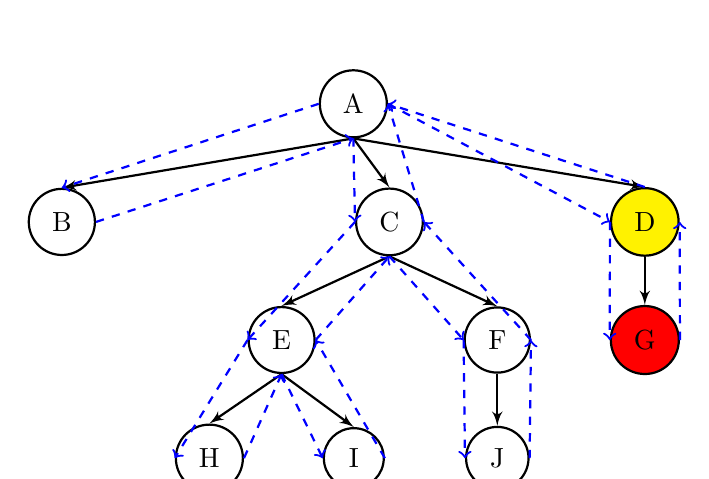
\begin{tikzpicture}[node distance=2cm and 4cm, level distance=1.5cm, 
    sibling distance=10mm,
        every node/.style={draw, thick, circle,inner sep=5pt, node 
        distance=2cm},
        every path/.style={->, draw, thick, -latex'}]
    \Tree [. \node(nodeA){A}; 
             [. \node(nodeB){B}; ]
             [. \node(nodeC){C};
                [. \node(nodeE){E};
                   [. \node(nodeH){H}; ]
                   [. \node(nodeI){I}; ]
                ]
                [. \node(nodeF){F};
                   [. \node(nodeJ){J}; ]
                ] 
             ]
             [. \node[draw, fill=yellow](nodeD){D};
                [ . \node[draw, fill=red](nodeG){G}; ]
             ] 
          ]
          
    \draw[blue, dashed, ->] (nodeA.west) -- 
                             (nodeB.north);
    \draw[blue, dashed, ->] (nodeB.east) -- 
                             (nodeA.south);
    \draw[blue, dashed, ->] (nodeA.south) -- 
                             (nodeC.west);
    \draw[blue, dashed, ->] (nodeC.west) -- 
                             (nodeE.west);
    \draw[blue, dashed, ->] (nodeE.west) -- 
                             (nodeH.west);
    \draw[blue, dashed, ->] (nodeH.east) -- 
                             (nodeE.south);
    \draw[blue, dashed, ->] (nodeE.south) -- 
                             (nodeI.west);
    \draw[blue, dashed, ->] (nodeI.east) -- 
                             (nodeE.east);
    \draw[blue, dashed, ->] (nodeE.east) -- 
                             (nodeC.south);
    \draw[blue, dashed, ->] (nodeC.south) -- 
                             (nodeF.west);
    \draw[blue, dashed, ->] (nodeF.west) -- 
                             (nodeJ.west);
    \draw[blue, dashed, ->] (nodeJ.east) -- 
                             (nodeF.east);
    \draw[blue, dashed, ->] (nodeF.east) -- 
                             (nodeC.east);
    \draw[blue, dashed, ->] (nodeC.east) -- 
                             (nodeA.east);
    \draw[blue, dashed, ->] (nodeA.east) -- 
                             (nodeD.west);
    \draw[blue, dashed, ->] (nodeD.west) -- 
                             (nodeG.west);
    \draw[blue, dashed, ->] (nodeG.east) -- 
                             (nodeD.east);
    \draw[blue, dashed, ->] (nodeD.north) -- 
                             (nodeA.east);

    \end{tikzpicture}
    \caption{Illustratie van een Euler traversal door een boom. Hier duiden 
    blauwe pijlen het pad aan dat doorheen de boom genomen wordt. De tabulaire 
    voorstelling van dit pad is te vinden in \Vref{tbl:euler}.}
    \label{tikz:eulertour}
\end{figure}

\begin{table}
	\centering
	\caption{Tabulaire voorstelling van een Euler traversal door de boom uit 
	\Vref{tikz:eulertour}.}
	\label{tbl:euler}
   	\begin{tabular}{cccccccccccccccccccc}
       	\toprule
       	Index & 0 & 1 & 2 & 3 & 4 & 5 & 6 & 7 & 8 & 9 & 10 & 11 & 12 & 
       	13 & 14 & 15 & 16 & 17 & 18 \\ 
       	\midrule
       	Node   & A & B & A & C & E & H & E & I & E & C & F & J & F & C & A 
       	& D & G & D & A \\ 
       	Diepte & 0 & 1 & 0 & 1 & 2 & 3 & 2 & 3 & 2 & 1 & 2 & 3 & 2 & 1 & 
       	0 & 1 & 2 & 1 & 0 \\ 
       	\bottomrule
   	\end{tabular} 
   	\vspace{1cm}
   	\caption{Tabel van eerste voorkomens van een node in \Vref{tbl:euler}.}
   	\label{tbl:firstocc}
    \begin{tabular}{cccccccccc}
        \toprule
        A & B & C & D & E & F & G & H & I & J \\ 
        \midrule
        0 & 1 & 3 & 15 & 4 & 10 & 16 & 5 & 7 & 11  \\ 
        \bottomrule
    \end{tabular} 
\end{table}

Eenmaal die tabel is opgesteld, kunnen we het RMQ algoritme toepassen op het
deel tussen node $u$ en node $v$ van de tabel. Het deel tussen die nodes kunnen
we vinden door gebruik te maken van de tabel van eerste voorkomens, weergegeven
in \Vref{tbl:firstocc}. Door de bijhorende indices te nemen van node $u$ en $v$,
kunnen we in \Vref{tbl:euler} RMQ toepassen op de lijst van dieptes van nodes
tussen deze indices. Ter illustratie kunnen we bijvoorbeeld de LCA berekenen van
nodes I en J. Nodes I en J komen volgens de tabel van eerste voorkomens
respectievelijk voor in de Euler traversal tabel op positie 7 en 11. De nodes
tussen I en J zijn dus [I, E, C, F, J] met respectievelijke dieptes [3, 2, 1, 2,
3]. De node met de laagste diepte is dus C.

Formeel samengevat gaat de reductie van een LCA probleem naar een RMQ probleem
als volgt (waarbij $n$ het aantal nodes in de boom is):

\begin{enumerate}
\item Stel de \texttt{euler\_tour} array van lengte $2*n-1$ op die de identifier
van de nodes bevat als we de boom langs het Euleriaanse pad aflopen;

\item Stel de \texttt{levels} array van lengte $2*n-1$ op waarbij $depth_i$
overeen komt met de diepte van overeenkomstige node \texttt{euler\_tour[i]};

\item Stel de \texttt{first\_occurences} array op van lengte $n$ op, waarbij
$first\_occurences[i]$ overeen komt met het eerste voorkomen van node $i$ in
\texttt{euler\_tour}.
\end{enumerate}

Het opstellen van die drie arrays kan in één depth-first traversal door de boom 
gebeuren. De voorbeeldcode hiervoor is terug te vinden in \Cref{lst:dfsrun} op 
\cpageref{lst:dfsrun}.

\begin{lstlisting}[caption={Voorbeeldcode om het LCA probleem te reduceren naar 
een probleem dat met RMQ kan worden opgelost.}, label={lst:dfsrun}, 
language=Python, float]
def dfs_run(self, taxon, iteration, level):

    euler_tour[iteration] = taxon.taxon_id
    levels[iteration] = level
    if not first_occurences[taxon.taxon_id]:
        first_occurences[taxon.taxon_id] = iteration

    for child in taxon.children:
        iteration = dfs_run(child, iteration + 1, level + 1)

        euler_tour[iteration] = taxon.taxon_id
        levels[iteration] = level

    return iteration + 1

euler_tour = [None]*(2*tree.length)-1)
levels = [None]*(2*tree.length)-1)
first_occurences = [None]*tree.length

dfs_run(root_taxon, 0, 0)
\end{lstlisting}

Wanneer deze drie arrays opgesteld zijn, komt het vinden van de LCA van twee 
nodes $u$ en $v$ neer op het volgende:

\begin{enumerate}

\item Zoek de index van $u$ en $v$ in de \texttt{first\_occurences} array. Dit
geeft \texttt{first\_occurences[u]} en \texttt{first\_occurences[v]} die de
positie van het eerste voorkomen van respectievelijk $u$ en $v$ in de
\texttt{euler\_tour} en de \texttt{levels} array aanduidt;

\item Bereken de RMQ in de subarray van \texttt{levels} van
\texttt{first\_occurences[u]} tot\\
\texttt{first\_occurences[v]}:
$\text{RMQ}_{levels}$(\texttt{first\_occurences[u]}:\texttt{first\_occurences[v]}).
Het resultaat hiervan is de index van de node met de kleinste diepte in de 
Euler traversal tussen $u$ en $v$;

\item De LCA van $u$ en $v$ bevindt zich nu in de \texttt{euler\_tour} array op
de index van het resultaat van voorgaande RMQ-bewerking:\\ LCA(u, v) =
\texttt{euler\_tour}[$\text{RMQ}_{levels}$(\texttt{first\_occurences[u]}:\texttt{first\_occurences[v]})].

\end{enumerate}

\subsubsection{RMQ}
De omzetting van het LCA probleem naar een RMQ probleem is dus zeker mogelijk in
lineaire tijd ten opzichte van de nodes in de boom. RMQ zelf is echter geen
eenvoudig probleem. In deze paragraaf wordt van een triviale implementatie
vertrokken en wordt gaandeweg een meer optimale oplossing bekomen, gebruik
makend van een aantal lemma's en observaties.

Er wordt gestart van een array $A$ van lengte $n$ met de eigenschap dat elk
element met $\pm1$ verschilt van zijn buren. De $\pm1$ beperking ontstaat
aangezien we het RMQ algoritme gebruiken op de \texttt{levels} array uit het
voorgaande deel. Het RMQ probleem op arrays waar niet aan die eigenschap is
voldaan, zullen we vanaf nu het RMQ probleem noemen. Wanneer wel aan deze
eigenschap is voldaan, noemen we dat het RMQ$\pm1$ probleem. In beide gevallen
blijft het doel om, gegeven twee indexen in lijst $A$, $i$ en $j$, de index van
de kleinste waarde in $A$ te bekomen tussen $i$ en $j$, met $i$ en $j$
inclusief.

\paragraph{Naïeve oplossing}
De naïeve oplossing is een oplossing die alle mogelijke combinaties van $i$ en
$j$ voorberekent. Deze oplossing heeft een complexiteit van $\Theta(n^3)$ om
alles voor te berekenen wat kan worden gereduceerd tot $\Theta(n^2)$ door
gebruik te maken van dynamisch programmeren. Het uitvoeren van de effectieve RMQ
vereist één lookup en kan dus in constante tijd gebeuren. Een preprocessing stap
van $\Theta(n^2)$ is echter veel te traag, zeker aangezien er snellere
algoritmes bestaan.
\paragraph{Snellere oplossing voor het algemene RMQ probleem} 
Er bestaat een snellere oplossing voor het algemene RMQ probleem. Het algemene
idee is om elke mogelijke query voor te berekenen waarvan de lengte een macht
van 2 is. Bij het opzoeken kunnen we dan de range opdelen in 2 (eventueel
overlappende) blokken waarvan de lengte een macht van 2 is. Om in constante tijd
tot een antwoord te komen, moeten we dus eerst voor elke $i$ tussen 1 en $n$ en
elke $j$ tussen 1 en $\log{n}$ het kleinste element van de deelarray startend
bij $i$ met lengte $2^j$ berekenen. Het resultaat hiervan voeren we in in de
tabel $M$ op positie $[i,j]$.  Formeel wordt dit: $M[i,j] = \min{\{A[k], k = i
.. i + 2^j - 1\}}$. Zo hebben we voor elke mogelijke startindex alle mogelijke
blokken binnen de array van een lengte van een macht van twee, startend op die
index. Voorgaande berekening is het eenvoudigst te begrijpen aan de hand van een
voorbeeld: voor de rij $[1, 6, 2, 4]$  van lengte 4, geeft dit het volgende
effect:

{ \centering
{ \footnotesize
\begin{tabular}{x{2cm}x{2cm}x{2cm}x{3cm}}
1 & 6 & 2 & 4\\

\cline{1-1}
\multicolumn{1}{l}{$M[1,0]=\min{A[1..1]}$} &  &  &  \\
\cline{1-2}
\multicolumn{2}{l}{$M[1,1]=\min{A[1..2]}$} &  &  \\
\cline{1-4}
\multicolumn{4}{l}{$M[1,2]=\min{A[1..4]}$}\\

\cline{2-2}
& \multicolumn{1}{l}{$M[2,0]=\min{A[2..2]}$}  &  & \\
\cline{2-3}
& \multicolumn{2}{l}{$M[2,1]=\min{A[2..3]}$}  & \\
\cline{2-4}
& \multicolumn{3}{l}{$M[2,2]=\min{A[2..5]}$}  \\

\cline{3-3}
& & \multicolumn{1}{l}{$M[3,0]=\min{A[3..3]}$}  & \\
\cline{3-4}
& & \multicolumn{2}{l}{$M[3,1]=\min{A[3..4]}$} \\
\cline{3-4}
& & \multicolumn{2}{l}{$M[3,2]=\min{A[3..6]}$}  \\

& & & ... \\
\end{tabular}
}
}

Met behulp van bovenstaande illustratie wordt duidelijk ingezien dat de
volledige matrix $M$ kan worden opgebouwd via dynamisch programmeren.

Formeel kan deze tabel opgebouwd worden volgens de formules, waarbij $M[i,j]$ 
met $j = 0$ overeen komt met het element op positie $i$ in $A$. 
\begin{equation*}
M[i,j] =
\begin{cases}
 M[i, j - 1], & \text{als } A[M[i,j - 1]] \leq A[M[i+2^{j - 1}-1, j - 1]]\\
 M[i + 2^{j-1}-1, j-1], & \text{anders} 
\end{cases}
\end{equation*}

In woorden omgezet betekent dit dat we in een blok van lengte $2^j$ het minimum
kunnen nemen van de blokken van lengte $2^{j-1}$ waaruit dit blok van lengte
$2^j$ is opgebouwd. In bovenstaand voorbeeld kunnen we zo $M[1,1]$ vinden door
het minimum te nemen van $M[1,0]$ en $M[2,0]$. Op dezelfde wijze kan $M[3,1]$
gevonden worden door het minimum te nemen van $M[3,0]$ en $M[4,0]$. Om dan
$M[1,2]$ te vinden, nemen we het minimum van $M[1,1]$ en $M[3,1]$ die we zonet
berekend hebben. Deze tabel kan dus worden opgevuld in $\Theta(n\log{n})$ tijd
en ruimte.

Voor bovenstaand voorbeeld ziet die tabel er dan als volgt uit:

\begin{tabular}{r|ccc}
	\toprule
	i & $j=0$ & $j=1$ & $j=2$ \\
	\midrule
	1 &   0   &   0   & 0     \\
	2 &   1   &   2   & 2     \\
	3 &   2   &   2   & 2     \\
	4 &   3   &   3   & 3     \\
	\bottomrule
\end{tabular}\\

De RMQ van een range van $i$ tot $j$ in $A$ kan nu gevonden worden door twee
(eventueel) overlappende blokken die deze volledige subarray bedekken. Om dat te
bekomen zoeken we eerst het grootste blok met een lengte van een macht 2 dat
binnen de subarray past. De lengte van dat blok kan eenvoudig berekend worden
met de formule $2^{\lceil \log(j - i) \rceil}$. De RMQ van die subarray vinden
we dan door het minimum te nemen van de RMQ op het blok dat start op index $i$ 
en
de RMQ van het blok dat eindigt op index $j$. Aangezien deze blokken een lengte
van een macht van 2 hebben, heeft de preprocessing de minima van die blokken al
voorberekend en kunnen we dus de RMQ in constante tijd berekenen van deze
arbitraire subarray.

In bovenstaand voorbeeld kunnen we bijvoorbeeld de RMQ berekenen van index 0 
tot 2. Hiervoor selecteren we twee blokken met lengte $2^{\lceil \log(2 - 0) 
\rceil} = 2$. Het eerste blok start op index 0, het laatste blok eindigt op 
index 2. De RMQ van deze twee blokken is al voorberekend: $A[M[1,1]] = A[0] = 
1$ en $A[M[2,1]] = A[2] = 2$. De oplossing is dus 1, te vinden in A op index 0.

Dit algoritme kan dus de array $A$ voorberekenen in $\Theta(n\log{n})$ tijd en
ruimte. Opzoekingen kunnen als gevolg van deze voorberekening in constante
snelheid gebeuren.

\paragraph{Oplossing voor het RMQ$\pm1$ probleem}
Het voorberekenen kan echter nog sneller wanneer de array $A$ voldoet aan de
$\pm1$ beperking. In het geval van de \texttt{levels} array is dat altijd zo
aangezien we altijd van kind naar ouder of omgekeerd gaan.

Eerst wordt de array $A$ verdeeld in blokken ter grootte van
$\frac{\log{n}}{n}$. Daarna wordt een array, $A'$ gedefinieerd van
$\frac{2*n}{\log{n}}$ elementen, waarbij het element op index $i$ in $A'$ het
minimum element is van het $i^\text{de}$ blok in $A$. Aangezien het RMQ
algoritme de index van het kleinste element in een array teruggeeft en niet de
waarde zelf, wordt een bijhorende array gedefinieerd, $B$ waar $B_i$ de positie
aangeeft van het kleinste element in het $i^\text{de}$ blok van $A'$.

Nu kan voorgaand algoritme voor het algemene RMQ probleem toegepast worden op 
de nieuwe array $A'$. Aangezien $A'$ van lengte $\frac{2*n}{\log{n}}$ is en 
het RMQ algoritme een tijdscomplexiteit heeft van $n * \log{n}$, gebeurt dit in 
$\Theta\left[\frac{2*n}{\log{n}} * \log{\frac{2*n}{\log{n}}}\right] \approxeq 
\Theta(n)$ tijd.

Op basis van de huidige preprocessing van $A'$ kunnen alle combinaties van $i$
en $j$ in constante tijd gevonden worden wanneer $i$ en $j$ op de grenzen van de
blokken in A vallen. Dit is echter niet altijd het geval. Aangezien $i$ en $j$
binnen eenzelfde blok kunnen vallen, moeten we ook elk blok apart voorberekenen.
Het is echter ook mogelijk dat $i$ en $j$ in verschillende blokken vallen. In
dat geval wordt de RMQ als volgt berekend:

\begin{enumerate}
\item Bereken het minimum van $i$ tot het einde van het blok waar $i$ in valt;
\item Bereken het minimum van alle blokken in $A$ tussen de blokken waar $i$ en
$j$ in vallen; 
\item Bereken het minimum van $j$ tot het begin van het blok waar $j$ in valt.
\end{enumerate}

Het minimum van deze drie waarden is dan het kleinste element binnen de array
$A$ tussen $i$ en $j$. Om stap 2 te berekenen kan gebruik worden gemaakt van de
reeds voorberekende array $A'$. Stap 1 en 3 vergen echter wat meer werk. Er moet
nu een snelle manier worden gevonden om een RMQ probleem te beantwoorden
binnenin één blok.

Als op elk blok in $A$ apart de algemene RMQ preprocessing zou worden gedaan,
zouden we te veel tijd spenderen aan preprocessing. Daarom wordt gekeken of we
het aantal mogelijke blokken kunnen beperken. Dat kan ook volgens
volgende observatie: Wanneer twee arrays, $X$ en $Y$, beide van lengte $k$, op
elke positie met een constante waarde verschillen zodat $X_i = Y_i + c$ voor
elke $i$ en een constante $c$, dan zijn alle mogelijke RMQ antwoorden hetzelfde
voor beide arrays. Bijvoorbeeld gegeven arrays $[1, 2, 1, 0]$ en $[3, 4, 3, 2]$
dan geldt deze observatie voor $c = 2$. In beide blokken is het resultaat van de
RMQ voor het volledige blok gelijk, namelijk index 3.

Deze observatie heeft een belangrijk gevolg. Nu kunnen we namelijk elk blok 
normaliseren door de eerste waarde uit dat blok af te trekken van alle waarden 
in datzelfde blok. Voor het voorbeeld hierboven geeft dit
$[1-1, 2-1, 1-1, 0-1] = [3-3, 4-3, 3-3, 2-3] = [0, 1, 0, -1]$. 

Er kan nu worden aangetoond dat er $\Theta(\sqrt{n})$ verschillende
genormaliseerde blokken kunnen bestaan. Alle genormaliseerde blokken starten
namelijk met $0$ aangezien die waarde van zichzelf wordt afgetrokken. Wegens de
$\pm1$ beperking die ook op deze genormaliseerde blokken geldt, bekomen we
strings van lengte $\frac{\log{n}}{2} - 1$, waarbij $n$ nog steeds de lengte is
van de originele array $A$. Deze genormaliseerde blokken kunnen we ook omzetten
in bitstrings waarbij een 1 aangeeft dat het getal op die index 1 hoger is dan
zijn voorgaande getal, en 0 op dezelfde manier een verschil van -1 aangeeft. Dit
resulteert in het bestaan van $2^{\frac{\log{n}}{2} - 1} = \frac{\sqrt{n}}{2} =
\Theta(\sqrt{n})$ bitstrings, en dus $\Theta(\sqrt{n})$ mogelijke
genormaliseerde blokken.

Wat nu nog rest is het maken van tabellen voor elk genormaliseerd blok. Voor 
deze
$\Theta(\sqrt{n})$ blokken wordt een tabel aangemaakt waarin we alle antwoorden
voor RMQ opvragingen binnen dat blok opslaan. Dit zijn er $\frac{\log{n}}{2}^2 =
\Theta\left(\log{n}^2\right)$ per blok, dus
$\Theta\left(\sqrt{n}\log{n}^2\right) \approxeq \Theta(n)$ in totaal.
Opzoekingen kunnen aan de hand van deze tabellen in constante tijd gebeuren.

Het laatste wat ons nog rest is het berekenen van welk blok in de originele 
array $A$ bij welk genormaliseerd blok hoort. Dit kan eenvoudig door een 
mapping bij te houden van de bitstring na normalisatie.

Samengevat hebben we nu binnen een tijdscomplexiteit van $\Theta(n)$
alle mogelijke RMQ$\pm1$ vragen binnen blokken voorberekend, alsook alle RMQ
vragen over meerdere blokken heen in dezelfde tijd. Door die voorberekening
kunnen we in constante tijd de drie benodigde minima opvragen zoals hierboven
aangegeven, en kunnen we nu voor eender welke opgegeven indices $i$ en $j$ het
RMQ$\pm1$ probleem oplossen in $\Theta(1)$. 

De omzetting van LCA naar RMQ kan door middel van de depth-first traversal in
$\Theta(n)$ gebeuren en dient éénmalig te gebeuren om de benodigde arrays  voor
de RMQ preprocessing voor te berekenen. De opslag voor zowel de benodigde arrays
van de boomstructuur als voor de de interne arrays in de RMQ preprocessing
bedraagt $\Theta(n)$.

\paragraph{Implementatie} 

Aangezien er enkele C bibliotheken bestaan die bovenstaand algoritme voor het
RMQ probleem implementeren, zullen we gebruik maken van zo'n bestaande
bibliotheek. De bibliotheek die we hiervoor gebruiken is een implementatie
geschreven door Hideo Bannai \cite{Hideo0:online, Hideo1:online} die voldoet aan
de besproken snelheids- en ruimtecomplexiteiten. Het berekenen van de
LCA van twee nodes gebeurt dan zoals geïllustreerd in \Vref{lst:lcaexample}.

\begin{lstlisting}[language=Python, caption={Voorbeeldcode in Python voor de 
LCA berekening van 2 nodes, na uitvoering van \Vref{lst:dfsrun}},
label={lst:lcaexample}, float]
def calc_lca_pair(first, second):
    first_index = first_occurences[first]
    second_index = first_occurences[second]
    
    rmq_index = get_rmq(first_index, second_index)
    
    return euler_tour[rmq_index]
\end{lstlisting}

\subsubsection{LCA van meerdere nodes} 

Met voorgaand algoritme kan gemakkelijk de LCA van twee nodes berekend worden.
Het probleem wordt echter moeilijker wanneer we de LCA van meer dan twee nodes
willen berekenen.

In een boomstructuur waar een interne orde opgelegd is, zouden we de boom
in-order kunnen overlopen. Daarna kunnen we uit alle querynodes de twee nodes
opzoeken die het eerst en het laatst voorkomen tijdens deze in-order wandeling
door de boom. Dit garandeert dat de twee geselecteerde nodes de buitenste nodes
van alle querynodes zijn, en dat dus enkel de LCA van deze twee nodes moet
berekend worden om tot een eindresultaat te komen voor alle querynodes.

Met deze aanpak zijn er echter twee aspecten die we in rekening moeten brengen.
Ten eerste is het niet mogelijk een vaste volgorde op te leggen aan de taxa in
de NCBI taxonomy. Enkel de kind-ouder relatie bestaat hier. Hoe een kind zich
verhoudt ten opzichte van ouder of broers is niet vastgelegd. Het proberen
opstellen van een in-order volgorde van een ouder met twee kinderen, A en B, kan
dus resulteren in zowel [A, ouder, B] als [B, ouder, A]. Wanneer de LCA(A,
ouder, B) berekend wordt, zal afhankelijk van de volgorde LCA(A, B) of LCA(B, A)
berekend worden, wat wegens het symmetrisch zijn van LCA hetzelfde resultaat
oplevert.

Ook belangrijk is dat de taxonomische boom geen binaire boom is. Stel dat de
voorgaande ouder er nog een kind bij krijgt, C, dan kan het in-order overlopen
volgende volgordes aannemen: [A, ouder, B, C], [A, B, ouder, C], [C, B, ouder,
A], et cetera. Als we dan opnieuw de LCA berekenen van LCA(A, ouder, B) dan
weten we niet of we LCA(A, B), LCA(A, ouder), LCA(B, A), ... moeten berekenen.
Ook hier leveren alle mogelijkheden hetzelfde resultaat op, namelijk de ouder, 
maar
we zullen later zien dat dit bij het LCA* algoritme niet het geval is.

\subsection{Van LCA naar LCA*} 

De aanpassing van LCA naar LCA* lijkt op het eerste zicht vrij eenvoudig. Als we
de LCA berekenen van twee nodes, en het resultaat van deze berekening is één van
die twee nodes, dan weten we dat beide nodes op hetzelfde pad naar de wortel
liggen. Als resultaat nemen we dan de node met de grootste diepte in plaats van
deze met de kleinste diepte in het geval van LCA*. De code die de LCA berekent
uit \Vref{lst:lcaexample} wordt dan uitgebreid naar de code in
\Vref{lst:lca*example}.

\begin{lstlisting}[language=Python, caption={Uitbreinding van de voorbeeldcode 
uit \Vref{lst:lcaexample} in Python voor de LCA* berekening van 2 nodes}, 
label={lst:lca*example}, float]
def calc_lca_pair(first, second):
    first_index = first_occurences[first]
    second_index = first_occurences[second]
    
    rmq_index = get_rmq(first_index, second_index)
    
    # Speciaal geval LCA*
    if rmq_index == first_index:
        lca_index = second_index
    elif rmq_index == second_index:
        lca_index = first_index
    # Wanneer de RMQ index geen van beide originele indexen is, gebruik LCA
    else:
        lca_index = rmq_index
    
    return euler_tour[lca_index]
\end{lstlisting}

Deze aanpassing levert echter problemen op voor het toepassen van het LCA*
algoritme wanneer de LCA wordt berekend van meer dan twee nodes. Zoals uitgelegd
in de vorige sectie, kan de LCA van meer dan twee nodes gevonden worden door het
LCA algoritme toe te passen op de eerste en laatste querynode bij een in-order
overlopen van de boom.

Stel dat we de boom er terug bij nemen met een ouder en drie kinderen: A, B en C
en de ordening [A, B, ouder, C]. LCA*(ouder, A, B) met de methode van het nemen
van de ``buitenste'' querynodes reduceert het probleem naar LCA*(A, ouder) wat
met voorgaand algoritme resulteert in A. Hier is echter de informatie uit de tak
van B verdwenen, A kan namelijk nooit het resultaat zijn van LCA*(A, B). Ook een
pre- en post-ordening hebben hetzelfde probleem, aangezien er geen specifieke
ordening vast ligt voor de taxonomische boom. Bijvoorbeeld met de pre-ordening
[ouder, A, B, C] is de LCA*(ouder, B, C) = LCA*(ouder, C) = C, waarbij de tak
van B opnieuw onterecht wordt genegeerd. Als laatste middel kunnen we nog terug
proberen te vallen op de Eulertraversal ordening, [ouder, A, ouder, B, ouder, C,
ouder], maar ook hier geldt het tegenvoorbeeld: LCA*(ouder, A, B) = LCA*(ouder,
B) = B, waarbij ditmaal de tak van A genegeerd wordt.

Een alternatief is het paarsgewijs toepassen van het LCA*-algoritme. Gegeven een
lijst van nodes kunnen we eerst voor de eerste twee nodes in die lijst de LCA*
berekenen. Het resultaat daarvan kan dan met LCA* geaggregeerd worden met de
derde node in de lijst. Op deze manier worden verder gegaan tot alle nodes in de
lijst zijn geaggregeerd. Grote lijsten kunnen op die manier zelfs parallel
verwerkt worden. Zo kan LCA*(A, B, C, D) bijvoorbeeld berekend worden aan de
hand van LCA*(LCA*(A, B), LCA*((C, D)). Voor het klassieke LCA-algoritme werkt
dit probleemloos aangezien we nooit in de boom afdalen. Dit is echter niet het
geval bij het LCA*-algoritme. In \Vref{fig:lca*hij} berekenen we bijvoorbeeld
LCA*(H, I, J). Dit wordt paarsgewijs berekend door eerst LCA*(H, I) = E te
berekenen en daarna LCA*(E, J) = C. Wanneer we echter een verkeerd
tussenresultaat op hetzelfde pad als een volgende node bekomen, zoals in
\Vref{fig:lca*bcd}, dan kan dit een verkeerd resultaat opleveren. LCA*(B, C, D)
wordt berekend aan de hand van LCA*(B, C) = A, en daarna LCA*(A, D). Dit levert
dat de lager liggende node D als LCA* resultaat, waardoor de takken van B en C
volledig genegeerd worden en het resultaat eveneens fout is.

\begin{figure}
	\centering
    \begin{subfigure}{0.45\linewidth}
        \centering
        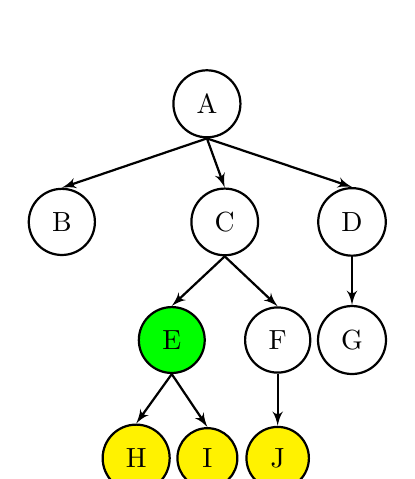
\begin{tikzpicture}[node distance=3cm, level distance=1.5cm,
            every node/.style={draw, thick, circle,inner sep=5pt},
            every path/.style={->, draw, thick, -latex'}]
        \Tree [. A 
                 [. B ]
                 [. C
                    [. \node[draw, fill=green]{E};
                       [. \node[draw, fill=yellow]{H}; ]
                       [. \node[draw, fill=yellow]{I}; ]
                    ]
                    [. F
                       [. \node[draw, fill=yellow]{J}; ]
                    ] 
                 ]
                 [. D
                    [ . G ]
                 ] 
              ]
        \end{tikzpicture}
        \caption{}
        \label{tikz:lca*hij}
    \end{subfigure}
    \begin{subfigure}{0.45\linewidth}
        \centering
        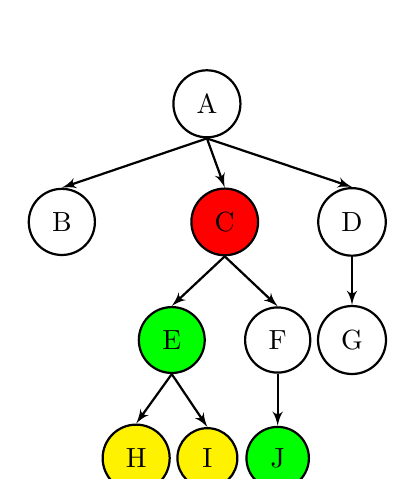
\begin{tikzpicture}[node distance=3cm, level distance=1.5cm,
            every node/.style={draw, thick, circle,inner sep=5pt},
            every path/.style={->, draw, thick, -latex'}]
        \Tree [. A 
                 [. B ]
                 [. \node[draw, fill=red]{C};
                    [. \node[draw, fill=green]{E};
                       [. \node[draw, fill=yellow]{H}; ]
                       [. \node[draw, fill=yellow]{I}; ]
                    ]
                    [. F
                       [. \node[draw, fill=green]{J}; ]
                    ] 
                 ]
                 [. D
                    [ . G ]
                 ] 
              ]
        \end{tikzpicture}
        \caption{}
        \label{tikz:lca*hij2}
    \end{subfigure}
    \caption{Tussenstappen voor berekenen van  LCA*(H, I, J). Gele nodes zijn
    querynodes, groene tussenresultaten en rode het eindresultaat. Via de
    iteratieve reductie geeft dit LCA*(LCA*(H, I), J), wat resulteert in LCA*(E,
    J). Het uitrekenen hiervan geeft C als correct resultaat.} 
    \label{fig:lca*hij}
\end{figure}

\begin{figure}
	\centering
    \begin{subfigure}{0.33\linewidth}
        \centering
        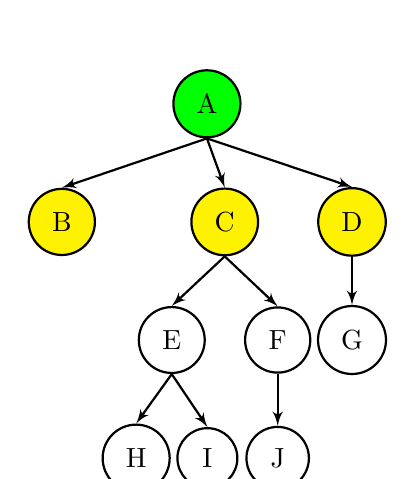
\begin{tikzpicture}[node distance=3cm, level distance=1.5cm,
            every node/.style={draw, thick, circle,inner sep=5pt},
            every path/.style={->, draw, thick, -latex'}]
        \Tree [. \node[draw, fill=green]{A}; 
                 [. \node[draw, fill=yellow]{B}; ]
                 [. \node[draw, fill=yellow]{C};
                    [. E
                       [. H ]
                       [. I ]
                    ]
                    [. F
                       [. J ]
                    ] 
                 ]
                 [. \node[draw, fill=yellow]{D};
                    [ . G ]
                 ] 
              ]
        \end{tikzpicture}
        \caption{}
        \label{tikz:lca*bcd1}
    \end{subfigure}
    \begin{subfigure}{0.33\linewidth}
        \centering
        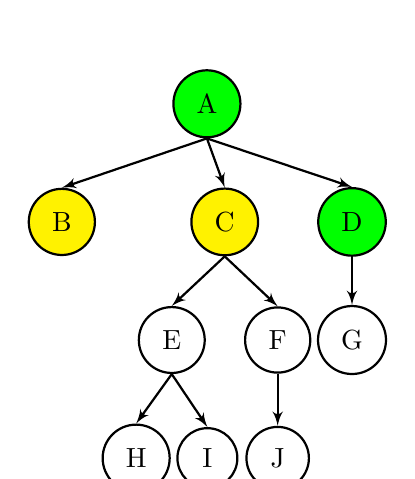
\begin{tikzpicture}[node distance=3cm, level distance=1.5cm,
            every node/.style={draw, thick, circle,inner sep=5pt},
            every path/.style={->, draw, thick, -latex'}]
        \Tree [. \node[draw, fill=green]{A}; 
                 [. \node[draw, fill=yellow]{B}; ]
                 [. \node[draw, fill=yellow]{C};
                    [. E
                       [. H ]
                       [. I ]
                    ]
                    [. F
                       [. J ]
                    ] 
                 ]
                 [. \node[draw, fill=green]{D};
                    [ . G ]
                 ] 
              ]
        \end{tikzpicture}
        \caption{}
        \label{tikz:lca*bcd2}
    \end{subfigure}
    \begin{subfigure}{0.33\linewidth}
        \centering
        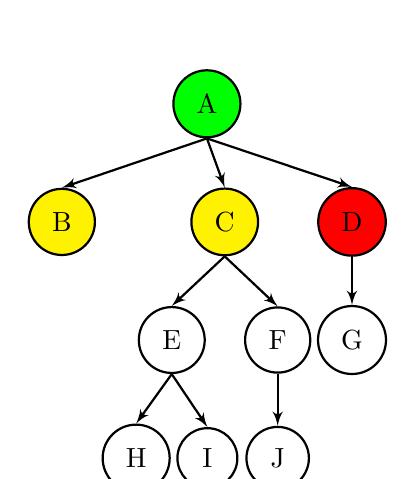
\begin{tikzpicture}[node distance=3cm, level distance=1.5cm,
            every node/.style={draw, thick, circle,inner sep=5pt},
            every path/.style={->, draw, thick, -latex'}]
        \Tree [. \node[draw, fill=green]{A}; 
                 [. \node[draw, fill=yellow]{B}; ]
                 [. \node[draw, fill=yellow]{C};
                    [. E
                       [. H ]
                       [. I ]
                    ]
                    [. F
                       [. J ]
                    ] 
                 ]
                 [. \node[draw, fill=red]{D};
                    [ . G ]
                 ] 
              ]
              
              
        \end{tikzpicture}
        \caption{}
        \label{tikz:lca*bcd3}
    \end{subfigure}
    \caption{Tussenstappen voor het berekenen van LCA*(B, C, D). Gele nodes zijn
    querynodes, groene tussenresultaten en rode het eindresultaat. Via de
    iteratieve methode geeft dit LCA*(LCA*(B, C), D), wat resulteert in LCA*(A,
    D). Het uitwerken van LCA*(A, D) geeft echter foutief D als resultaat
    waarbij de takken van B en C volledig genegeerd worden.}
    \label{fig:lca*bcd}
\end{figure}

De oorzaak van het probleem is te wijten aan het afdalen in de boom met het LCA*
algoritme wanneer een eerder bekomen LCA* resultaat als tussenstap gebruikt
wordt. Om dit probleem op te lossen, kan gebruik gemaakt worden van een
dieptelimiet in de boom, waar niet onder mag worden afgedaald. Deze dieptelimiet
schuift telkens op naar het niveau van een node die het resultaat is van een
LCA* tussenstap waar niet wordt afgedaald. In het voorbeeld in
\Vref{tikz:lca*bcd2} zou bij de berekening van LCA*(B, C, D) = LCA*(LCA*(B, C),
D) er na het verkrijgen van A als tussenresultaat van LCA*(B, C) dus niet verder
mogen worden afgedaald worden in een tak onder A, aangezien A reeds het
tussenresultaat is van een gewone LCA stap op B en C. Na deze stap wordt de
dieptelimiet op 0 gezet, aangezien resultaat A diepte 0 heeft. Wanneer een
volgende LCA* stap gedaan wordt op A en D, met dieptelimiet 0, dalen we niet af
naar D aangezien de diepte van D (1) groter is dan deze limiet (0). Dit wordt
geïllustreerd in \Vref{tikz:lcafix*bcd}. De nieuwe notatie die we hiervoor
invoeren is $\text{LCA}_d$* waarbij $d$ de huidige waarde is van de
dieptelimiet. LCA*($n_1$,$n_2$,...,$n_m$) is dan een korte notatie voor 
$\text{LCA}_\infty$*($n_1$,$n_2$,...,$n_m$).

\begin{figure}
	\centering
    \begin{subfigure}{0.33\linewidth}
        \centering
        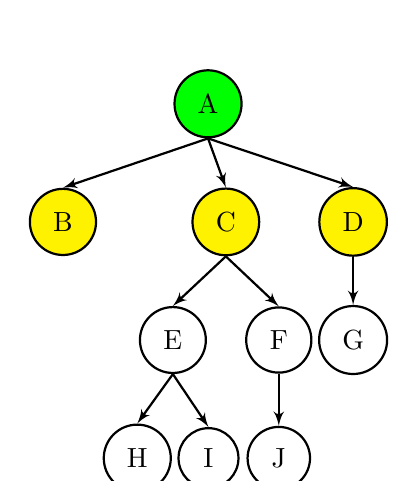
\begin{tikzpicture}[node distance=3cm, level distance=1.5cm,
            every node/.style={draw, thick, circle,inner sep=5pt},
            every path/.style={->, draw, thick, -latex'}]
        \Tree [. \node[draw, fill=green]{A}; 
                 [. \node[draw, fill=yellow](nodeB){B}; ]
                 [. \node[draw, fill=yellow]{C};
                    [. E
                       [. \node(nodeH){H}; ]
                       [. I ]
                    ]
                    [. F
                       [. J ]
                    ] 
                 ]
                 [. \node[draw, fill=yellow](nodeD){D};
                    [ . G ]
                 ] 
              ]
              
          \draw[red, dashed, -] 
              (nodeH.south -| nodeB.west) -- 
              (nodeH.south -| nodeD.east);
        \end{tikzpicture}
        \caption{}
        \label{tikz:lcafix*bcd1}
    \end{subfigure}
    \begin{subfigure}{0.33\linewidth}
        \centering
        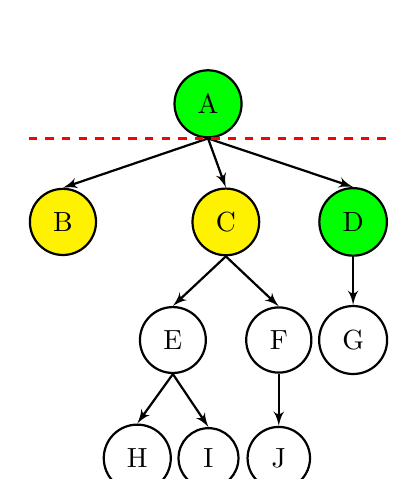
\begin{tikzpicture}[node distance=3cm, level distance=1.5cm,
            every node/.style={draw, thick, circle,inner sep=5pt},
            every path/.style={->, draw, thick, -latex'}]
        \Tree [. \node[draw, fill=green](nodeA){A}; 
                 [. \node[draw, fill=yellow](nodeB){B}; ]
                 [. \node[draw, fill=yellow](nodeC){C};
                    [. E
                       [. \node(nodeH){H}; ]
                       [. I ]
                    ]
                    [. F
                       [. J ]
                    ] 
                 ]
                 [. \node[draw, fill=green](nodeD){D};
                    [ . G ]
                 ] 
              ]
              
            \draw[red, dashed, -] 
                (nodeA.south -| nodeB.west) -- 
                (nodeA.south -| nodeD.east);
        \end{tikzpicture}
        \caption{}
        \label{tikz:lcafix*bcd2}
    \end{subfigure}
    \begin{subfigure}{0.33\linewidth}
        \centering
        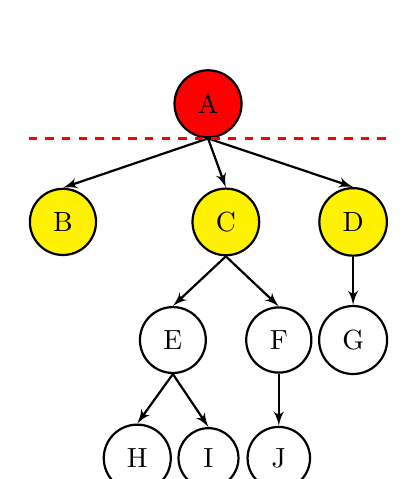
\begin{tikzpicture}[node distance=3cm, level distance=1.5cm,
            every node/.style={draw, thick, circle,inner sep=5pt},
            every path/.style={->, draw, thick, -latex'}]
        \Tree [. \node[draw, fill=red](nodeA){A}; 
                 [. \node[draw, fill=yellow](nodeB){B}; ]
                 [. \node[draw, fill=yellow](nodeC){C};
                    [. E
                       [. H ]
                       [. I ]
                    ]
                    [. F
                       [. J ]
                    ] 
                 ]
                 [. \node[draw, fill=yellow](nodeD){D};
                    [ . G ]
                 ] 
              ]
              
              \draw[red, dashed, -] 
                  (nodeA.south -| nodeB.west) -- 
                  (nodeA.south -| nodeD.east);
              
        \end{tikzpicture}
        \caption{}
        \label{tikz:lcafix*bcd3}
    \end{subfigure}
    \caption{Tussenstappen voor het berekenen van $\text{LCA}_\infty$*(B, C, D).
    Gele nodes zijn querynodes, groene tussenresultaten en rode het
    eindresultaat. Met de paarsgewijze methode geeft dit 
    $\text{LCA}_0$*($\text{LCA}_\infty$*(B, C), D). De binnenste LCA* 
    berekening geeft A als resultaat. Aangezien B en C beide 
    deeltakken zijn van A wordt de dieptelimiet naar boven geschoven tot op de 
    diepte van A, namelijk 0. Dit resulteert in $\text{LCA}_0$*(A, D). Het 
    uitwerken hiervan zou met de oude methode D als resultaat geven, maar 
    aangezien de diepte van D groter is dan de dieptelimiet geven we A als 
    resultaat.}
    \label{tikz:lcafix*bcd}
\end{figure}

We breiden nu het codevoorbeeld uit \Vref{lst:lca*example} uit naar 
\Vref{lst:lcafix*example}, waarin rekening wordt gehouden met de dieptelimiet.

\begin{lstlisting}[language=Python, caption={Uitbreinding van de voorbeeldcode 
uit \Vref{lst:lca*example} in Python voor de LCA* berekening van 2 nodes. Deze 
code houdt rekening met de toegevoegde \texttt{depth\_limit} parameter. Zoals 
besproken kan de \texttt{reduce} stap hier ook geparallelliseerd worden in 
plaats van met een accumulator te werken.}, 
label={lst:lcafix*example}]
def calc_lca_pair(acc, second, depth_limit):
    depth_limit, first = acc

    first_index = first_occurences[first]
    second_index = first_occurences[second]
    
    rmq_index = get_rmq(first_index, second_index)
    
    # Speciaal geval LCA*
    if rmq_index == first_index and levels[second_index] <= depth_limit:
        lca_index = second_index
    elif rmq_index == second_index and levels[first_index] <= depth_limit:
        lca_index = first_index
    # Wanneer de RMQ index geen van beide originele indexen is, gebruik LCA
    else:
        lca_index = rmq_index
        depth_limit = levels[lca_index]
    
    return (euler_tour[lca_index], depth_limit)
    

# Input: een lijst (of generator) van taxon identifiers
taxon_ids = iter([...])

first = next(taxon_ids)
depth_limit = sys.maxsize

_, lca_id = reduce(calc_lca_pair, taxon_ids, (depth_limit, first))

\end{lstlisting}

\section{Toekomstig werk}

In dit hoofdstuk bespraken we een nieuwe aggregatiemethode om verschillende taxa
te aggregeren tot een zo specifiek mogelijk eindresultaat om te gebruiken bij de
analyse van metagenomic samples. Deze nieuwe methode moet natuurlijk wel ergens
kunnen worden gebruikt. De aangewezen plaats is hiervoor zijn de Unipept web
services, zodat deze door zowel de Unipept command-line interface als door de
webinterface kan gebruikt worden. In deze webservices is inmiddels al het
commando \texttt{taxa2lca}\cite{taxa2lca:online} ingebouwd, die gebruik maakt
van de huidige tabelgebaseerde berekening. Analoog aan dit commando zou dus een
nieuwe commando, \texttt{taxa2treelca} kunnen worden ingebouwd.  Aangezien alle
calls naar deze services zo snel mogelijk moeten gebeuren, zou het dus
aangeraden zijn dat de Unipept webservices de benodigde data voor het RMQ
probleem in memory houden zodat een LCA* vraag onmiddellijk kan worden
beantwoord zonder dat er nog iets moet worden opgestart of opgebouwd.

Als alternatief voor onderzoekers die hun data niet graag over het internet
sturen kunnen we ook een lokale versie van dit commando aanbieden. Dit houdt
natuurlijk wel in dat de gebruiker de benodigde arrays en preprocessing lokaal
moet doen. Voor de case study in \Vref{chap:casestudy} werden al enkele scripts
geschreven die een taxonomie kunnen inladen en deze omzetten in de benodigde
arrays en datastructuren om het LCA* probleem te kunnen oplossen. De gebruiker
zou er dan voor kunnen kiezen om zelf een service te draaien die deze
datastructuren in memory houdt, of om de voorberekende data te serialiseren
zodat deze niet telkens opnieuw hoeft voorberekend te worden.

Een laatste puntje dat verbeterd kan worden is het gebruik van de C bibliotheek.
Momenteel wordt deze vanuit Python opgeroepen, waardoor bij elke oproep naar die
bibliotheek de data moet worden omgezet van een Python datastructuur naar een C
datastructuur. Aangezien de Unipept web en command-line interface in Ruby
geschreven zijn zou die omzetting daar dus ook moeten gebeuren. Een
herimplementatie van die bibliotheek in native Python/Ruby code zou deze
omzetting, en dus ook het tijdsverlies dat ermee gepaard gaat, overbodig maken.
Of de resulterende native code dan ook werkelijk sneller is dan de omzetting
naar en de berekening in C zal gebenchmarkt moeten worden.
\chapter{Case Study: Benchmarking the Unipept Metagenomics Analysis Pipeline}
\chaptermark{Benchmarking the UMAP}
\label{chap:casestudy}

In dit hoofdstuk evalueren we de prestaties van de Unipept Metagenomics Analysis
Pipeline (UMAP). Dat werd onderzocht in een groepsproject van het vak
Computationele Biologie, gedoceerd door professor Dawyndt, door een groep van
vijf studenten (Robin Declerck, Simon Houbracken, Michael Niklaus, Ine
Melckenbeeck, Bereket Tesfamariam Habtemariam) onder leiding van mijzelf.

In een tweede project binnen het vak werden, onder leiding van Felix Van der
Jeugt, reeds geclassificeerde peptiden in de IGC databank opnieuw
geclassificeerd met de UMAP. Zij concludeerden dat het grootste deel van de
resultaten overeen kwamen tussen Unipept en IGC, maar dat Unipept meer (zowel
true als false) positives rapporteert en daarenboven ook een specifieker
onderscheid tussen de verschillende rangen maakt. Het volledige onderzoek is te
lezen in de scriptie: ``Optimaliseren van de Unipept Shotgun
Metaproteomics Analysis Pipeline''\cite{felixthesis}.

Ter herhaling doorloopt de UMAP enkele stappen, geïllustreerd in de inleiding in
\Vref{fig:van_naar}. Voor elke DNA read in een metagenomics sample kunnen we een
proteomics experiment doen. Hierbij zoeken we, bijvoorbeeld aan de hand van
FragGeneScan, alle eiwitten op de DNA read in kwestie. De bekomen eiwitten
worden opgedeeld in tryptische peptiden waarna elke peptide afzonderlijk op zijn
taxonomische identificatie wordt afgebeeld door middel van het lowest common
ancestor (LCA) algoritme. Aan de hand van het LCA* algoritme, beschreven in
\Vref{chap:lca*}, kunnen we de bekomen taxa aggregeren naar een
consensusclassificatie.

Voor dit benchmarkingsproces gaan we eerst op zoek naar een manier om te testen
hoe goed de UMAP presteert op ongekende data en stellen we een aantal kernvragen
die binnen dit onderzoek beantwoord moeten worden. Daarna worden de genomen
stappen in het onderzoek besproken en vatten we de resultaten samen. ``Goed
presteren'' definiëren we hier aan de hand van één hoofdzaak en enkele bijzaken.
De toolchain moet hoofdzakelijk een zo specifiek mogelijke, maar wel correcte,
identificatie van de invoerdata als resultaat geven. Daarnaast moet de
identificatie ook snel kunnen gebeuren zonder al te veel hardwarebenodigdheden
te vragen.

\section[Bepalen van een benchmarkstrategie]{Bepalen van een benchmarkstrategie%
  \sectionmark{Benchmarkstrategie}}
\sectionmark{Benchmarkstrategie}

Het bepalen van een benchmarkstrategie is cruciaal om tot betrouwbare resultaten
te komen. Op het eind van deze case study willen we drie vragen kunnen
beantwoorden: \textit{i)} hoe accuraat is taxonomische identificatie met de
UMAP, \textit{ii)} hoe accuraat is die taxonomische identificatie wanneer ze
wordt toegepast op onbekende data en \textit{iii)} hoe goed presteert de UMAP op
gesimuleerde DNA reads die fouten bevatten?

De eerste vraag kunnen we onderzoeken door bekende, volledig gesequeneerde
genomen als invoer van de UMAP te gebruiken. Aangezien alle data uit deze
genomen bekend is, en we er ook van uit gaan dat de taxonomische identificatie
van de genomen correct is, verwachten we dat de resultaten zeer specifiek zullen
zijn.

De tweede vraag is echter moeilijker te beantwoorden. We kunnen namelijk geen
analyse uitvoeren van nog niet gesequeneerde genomen, aangezien we dan geen
objectieve manier hebben om in te schatten hoe accuraat het resultaat van de
analyse zou zijn. Wat we wel kunnen, is dit soort genomen simuleren op basis van
de complete genomen uit de vraag hierboven. Wanneer we de \Vref{fig:workflow} er
nog eens bij halen, zien we dat in de Unipept Metaproteomics Analysis Pipeline
de LCA van een peptide wordt berekend aan de hand van de eiwitten waarin dit
peptide voorkomt. Deze eiwitten worden dan afgebeeld op hun overeenkomstige
taxa, waarna via een aggregatie via LCA een consensustaxon bekomen wordt. Stel
nu echter dat een genoom, en bij gevolg ook eiwitten uit dat genoom, niet
gekend is, dan zal de resulterende mapping van een peptide naar eiwitten die
eiwitten ook niet bevatten. Het proces van ``niet gekend zijn'' kunnen we dus
simuleren door alle eiwitten die voorkomen in het oorspronkelijk genoom te
schrappen uit de lijst van eiwitten bij een peptide horen. Door middel van deze
filterstap (soort van leave-one-out strategie) kunnen we dus een ongekend genoom
simuleren uit een wel gekend genoom en kunnen we toch nog de resultaten
vergelijken.

De derde vraag kan op de volgende manier beantwoord worden. We kunnen aan de
hand van een read simulator, zoals wgsim \cite{lh3/w4:online}, reads met
verschillende error percentages simuleren op basis van een volledig genoom. In
deze reads kunnen we dan via een gene predictor, bijvoorbeeld FragGeneScan
\cite{rho2010fraggenescan}, eiwitfragmenten extraheren. Op deze eiwitten kunnen
we kunnen we dan de UMAP uitvoeren en de resultaten vergelijken met de
resultaten van de UMAP op het originele genoom.

We werken dus twee benchmarks uit. In de eerste nemen we de sequentie van een
genoom als invoer, waaruit we alle eiwitten extraheren. Die eiwitten splitsen
we vervolgens op in peptiden, waarop de Unipept Metaproteomics Analysis Pipeline
wordt uitgevoerd. De resulterende lijst van taxa aggregeren we nu per proteïne
met het LCA* algoritme naar een consensustaxon. Als uitvoer krijgen we dan voor
elke proteïne in het invoergenoom een taxonomische identificatie die we kunnen
vergelijken met de taxonomische identificatie van het genoom zelf. Deze
toolchain noemen we in het vervolg \texttt{pept2lca2lca*}. De naamgeving hiervan
steunt op de genomen stappen in de analyse: van peptiden $\rightarrow$ lca en
van lca $\rightarrow$ lca*. In de volgende sectie zal deze naamgeving
verduidelijkt worden.

Bij de tweede toolchain nemen we opnieuw een genoom als invoer, waaruit we
opnieuw alle eiwitten extraheren. De eiwitten splitsen we op in peptiden. Deze
peptiden verwerken we op vergelijkbare wijze als hierboven, maar nu met een
bijkomende tussenstap. Voor elke peptide wordt eerst een lijst van eiwitten
opgevraagd waar het betreffende proteïne in voorkomt. Uit deze lijst worden dan
de eiwitten gefilterd die reeds voorkomen in het invoergenoom. De resterende
eiwitten worden verder verwerkt door ze af te beelden op hun taxa in de Unipept
taxonomie, waarna ze worden geaggregeerd via het LCA algoritme. De lijst van
resulterende taxa wordt vervolgens per proteïne geaggregeerd wordt de lijst van
resulterende taxa per proteïne geaggregeerd met het LCA* algoritme, wat een
zelfde lijst als bij de eerste toolchain oplevert. Naar deze toolchain verwijzen
we vanaf nu met \texttt{pept2prot2filter2lca}, steunend op de overgangen van
peptiden $\rightarrow$ eiwitten, eiwitten $\rightarrow$ gefilterde eiwitten,
gefilterde eiwitten $\rightarrow$ lca*.

Door één invoergenoom op beide manieren te verwerken, krijgen we nu één
consensustaxon per proteïne uit het genoom. Deze twee lijsten kunnen we nu
onderling vergelijken om na te gaan hoeveel er precies aan specificatie verloren
is gegaan door de filterstap. Voor een goede taxonomische identificatie door
UMAP verwachten we dat de eerste lijst (zonder filtering) bijna volledig zal
bestaan uit taxa op \textit{species} niveau. De tweede lijst (analyse op
gesimuleerde onbekende genomen) kunnen we dan vergelijken met de eerste lijst om
het verlies aan taxonomische identificatie in te schatten wanneer er wordt
gewerkt met ongekende genomen.

Op deze twee resulterende lijsten van taxa wordt ook een onderscheid gemaakt
tussen specificatieverlies en een verkeerde identificatie van een taxon. Wanneer
het resulterende taxon op de lineage ligt van het taxon van het genoom in de
invoer, maar niet van de rang \textit{species} is, verliezen we aan
specificatie. Dit zullen we aangeven met de term ``match''. Wanneer de
resulterende taxon niet op de lineage ligt van het taxon van het ingevoerde
genoom, spreken we van een verkeerde identificatie, of ``mismatch''.

Als invoer voor dit benchmarkingsproces gebruiken we een lijst van ruim duizend
volledig gesequeneerde genomen uit de NCBI databank. Beide toolchains worden
geïllustreerd in \Vref{fig:abstractimage}.

\begin{figure}
	\centering
	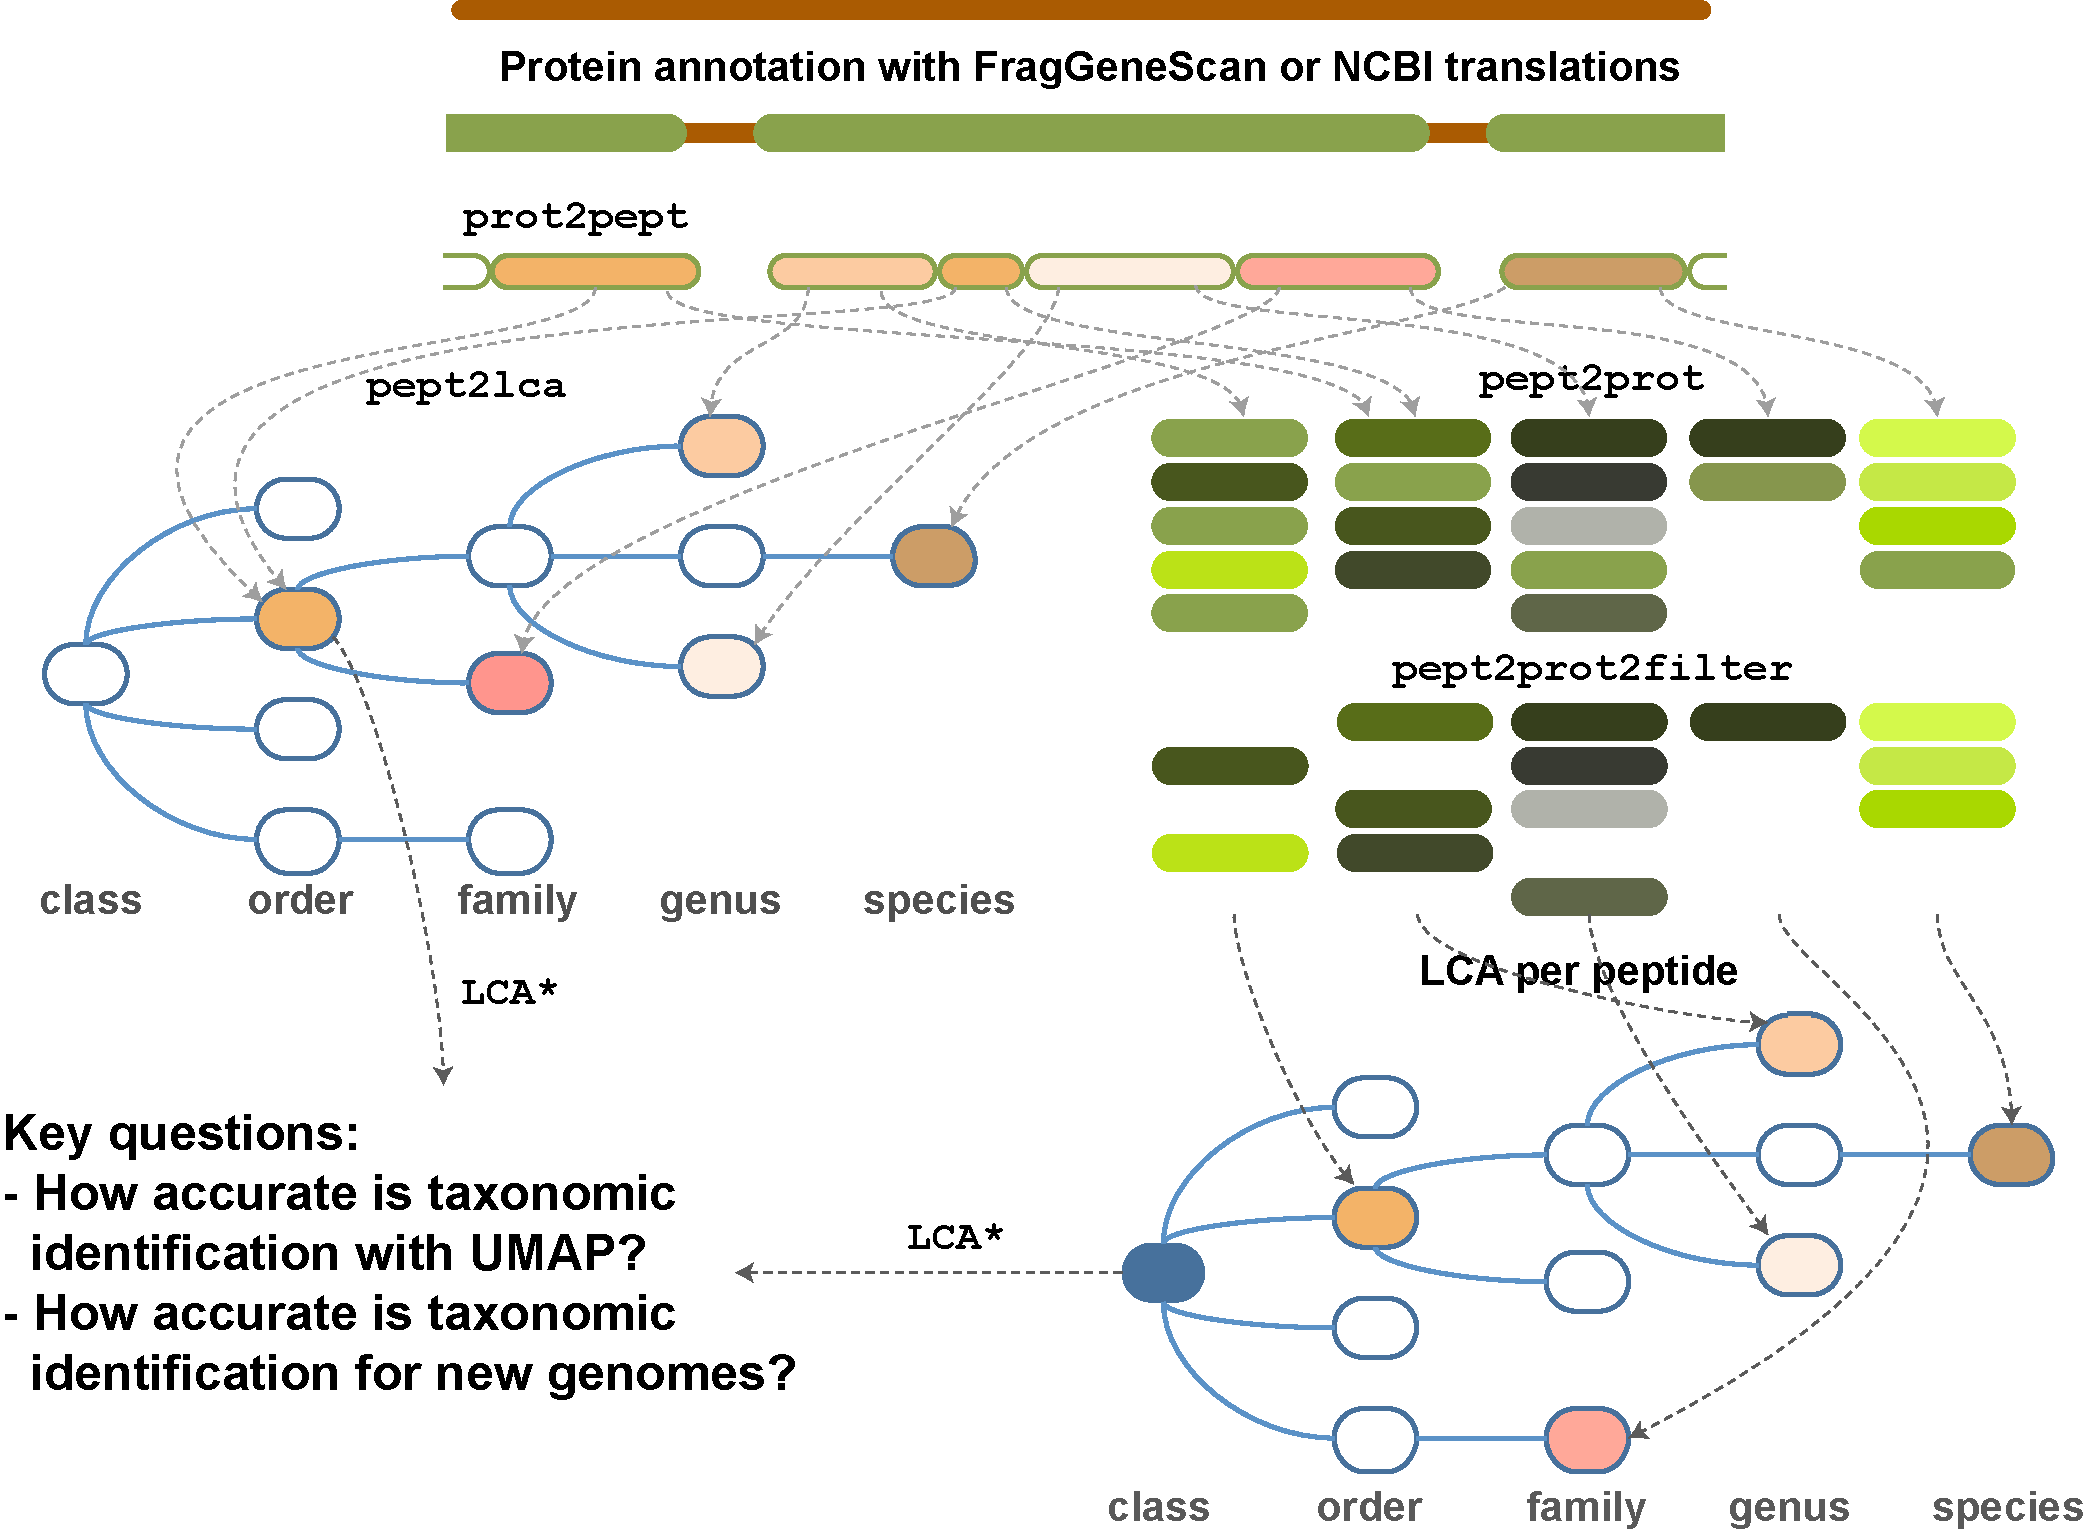
\includegraphics[width=0.8\textwidth]{includes/abstractimage.pdf}
	\caption{Illustratie van beide processen. Alle eiwitten worden uit een 
	genoom geëxtraheerd en opgesplitst in peptiden. Die peptiden worden dan 
	verwerkt via de Unipept Metaproteomics Analysis Pipeline tot taxa (links) 
	of worden (rechts) verwerkt door eerst alle eiwitten op te vragen waarin 
	de peptide voorkomt. Daarna wordt die lijst van eiwitten gefilterd op 
	eiwitten die voorkomen in het originele genoom. Vervolgens worden die 
	eiwitten afgebeeld via LCA op hun consensustaxa in de Unipept taxonomie. 
	Beide resulterende lijsten van taxa worden dan door een LCA* stap per 
	proteïne geaggregeerd en met elkaar vergeleken.}
	\label{fig:abstractimage}
\end{figure}

\section{Implementatie} 

De implementatie van de twee hierboven beschreven toolchains steunt op een 
aantal tools en bibliotheken. In deze sectie bespreken we eerst
deze lijst en geven we aan waar we de tools voor gebruiken. Daarna volgt de
bespreking van het benchmarkingsproces aan de hand van een analysescript.
Vervolgens staan we nog stil bij een ingreep in dat script om de snelheid ervan
te verhogen.

\subsection{Gebruikte tools en bibliotheken}

\begin{itemize}

\item \textbf{Unipept-CLI:} zoals beschreven in de inleiding is de Unipept-CLI
een interface in Ruby naar de webservices van Unipept. Hiermee kunnen alle
methodes van de Unipept webservices aangesproken worden. We maken gebruik van de
commando's \texttt{pept2lca}, die een lijst van peptides op hun LCA afbeeldt, en
\texttt{pept2prot} die voor een peptide een lijst van eiwitten oplevert waar
die peptide in voorkomt. Met de Ruby \texttt{unipept}-gem komen ook de
commando's \texttt{prot2pept}, die een een proteïne omzet in tryptische
peptides, en \texttt{peptfilter} die te lange (>50) of te korte (<5) peptides
filtert uit een lijst van opgegeven peptides.

\item \textbf{Biopython:} Biopython \cite{Biopy8:online} is een Python 
bibliotheek die een heel aantal tools voor computationele biologie bundelt. Wij 
zullen gebruik maken van de Entrez module \cite{Bio.E7:online}. Deze module 
zorgt ervoor dat we via de command-line toegang hebben tot de NCBI database om 
bijvoorbeeld alle eiwitten uit een genoom op te vragen.

\item \textbf{UniProt mapping:} De UniProt mapping \cite{Retri1:online} service
is een webservice die het vertalen van identifiers van eiwitten van en naar
overeenkomstige identifiers uit verschillende databanken vereenvoudigt. Deze
worden specifiek gebruikt om de identifiers van proteïne uit NCBI om te zetten
naar UniProtKB identifiers.

\item \textbf{RMQ-bibliotheek:} Een implementatie van een RMQ library
\cite{Hideo0:online, Hideo1:online} in C die voldoet aan de besproken snelheids-
en ruimtecomplexiteiten uit \Vref{chap:lca*}.

\item \textbf{Eigen scripts:} Deze scripts kunnen worden onderverdeeld in twee 
soorten:

    \begin{itemize}
    
    \item Een reeks van \textbf{wrapper scripts} in Bash en Python die hierboven
    benoemde tools wrappen. Deze zijn gemaakt om bijvoorbeeld alle eiwitten op
    te vragen van een NCBI assembly of bijvoorbeeld om het resultaat van de
    \texttt{pept2lca} stap te aggregeren via LCA*, gebruik makend van de
    RMQ-bibliotheek.
    
    \item \textbf{Ondersteunende scripts} die de volledige taxonomische boom
    inladen en aan de hand van die data de benodigde arrays voor de
    preprocessing van RMQ opstellen.
    \end{itemize}

\end{itemize}

\subsection{Implementatie van de benchmark} 

In dit gedeelte overlopen we een analysescript in Bash, dat alle stappen van het
volledige benchmarkingsproces uitvoert. De enige parameter waarmee dit script
moet worden aangeroepen is een GenBank accession number van een assembly. Dit
ziet er bijvoorbeeld uit als \texttt{GCA\_000015425.1}.
\begin{lstlisting}[language=Bash]
#!/bin/bash
asm_id=$1 && shift
\end{lstlisting}

Aangezien alle scripts verspreid staan over meerdere folders en we ook een
aantal (tussentijdse) resultaten wegschrijven, stellen we eerst enkele folders
in en maken we die aan waar nodig. De gebruiker kan kiezen om de
standaardwaarden van die folders te overschrijven aan de hand van opties van het
Bash script.

\begin{lstlisting}[language=Bash,firstnumber=3]
# Save directory of the analysis script to know where to find the others
dir="$(dirname "$0")"

# Create a tmpdir and a datadir
tmpdir=$(mktemp -d -t "$asm_id.XXXXXXXXXX")
datadir=$tmpdir
rmqdatadir=""

while getopts "d:t:r:" opt
do
  case $opt in
    d)
      datadir="$OPTARG/$asm_id"
      ;;
    t)
      tmpdir="$OPTARG/$asm_id"
      ;;
    r)
      rmqdatadir="-r $OPTARG"
      ;;
    ?)
      usage
      ;;
  esac
done

mkdir -p $datadir
mkdir -p $tmpdir

echo "Writing data to $datadir"
echo "Writing tempdata to $tmpdir"
\end{lstlisting}

De eerste stap is het ophalen van de taxon identifier van de assembly. Dit 
gebeurt aan de hand van het \texttt{asm2taxid} script, dat een wrapper is rond 
de Entrez module in BioPython. Het resultaat hiervan is bijvoorbeeld 400667 
voor genoemd GenBank accession number 

\begin{lstlisting}[language=Bash,firstnumber=34]
# get the taxon ID of the assembly
tax_id=$(python3 $dir/../entrez/asm2taxid.py $asm_id)
\end{lstlisting}

We moeten natuurlijk ook alle peptiden hebben als brondata voor een analyse. Dit
doen we aan de hand van het wrapperscript \texttt{asm2pept} dat, gegeven een
assembly identifier, de bijhorende eiwitten uit de NCBI databank opvraagt en
die eiwitten via de commando's \texttt{prot2pept} en \texttt{peptfilter} omzet
naar een lijst van peptiden. Deze peptiden worden gegroepeerd onder het id van
hun bijhorende proteïne opgeslagen in een FASTA bestand, genaamd
\texttt{peptides.fst}.

\begin{lstlisting}[language=Bash,firstnumber=36]
#  get the complete sequence and process it with:
#     - prot2pept
#     - peptfilter

echo "Getting peptides"
if [ ! -s "$tmpdir/peptides.fst" ]
then
  echo "No peptides found, downloading."
  python3 $dir/../entrez/asm2pept.py $asm_id > "$tmpdir/peptides.fst"
fi
\end{lstlisting}

Eens we de FASTA file van peptiden gegroepeerd hebben onder hun proteïne
identifier, kunnen we de eerste toolchain (de taxonomische identificatie
van volledige genomen) starten door \texttt{pept2lca} op dit bestand uit te
voeren. \texttt{pept2lca} vraagt aan de Unipept webservices voor elke peptide
zijn bijhorende taxonomische identificatie op. Het commando zorgt er ook voor
dat alles gegroepeerd blijft onder zijn FASTA header.

De uitvoer hiervan wordt naar het \texttt{pept2lca2lca} (vandaar ook de naam van
deze toolchain) commando gepiped. Het \texttt{pept2lca2lca} script is een
wrapperscript rond de RMQ-bibliotheek die voor de groepen van taxa onder een
proteïn identifier de LCA* berekent. Als optioneel argument neemt dit script een
taxon identifier. Wanneer deze taxon identifier wordt meegeleverd, voegt het
script een extra kolom toe aan de uitvoer die een 1 bevat wanneer resulterende
taxon een ``match'' is en 0 bevat wanneer de resulterende taxon een ``mismatch''
is.

De uitvoer wordt geschreven naar \texttt{pept2lca2lca.fst} wat het eindresultaat
is van de eerste toolchain.

\begin{lstlisting}[language=Bash,firstnumber=46]
# analyse the complete sequence with and
# check whether resulting taxa come from the correct lineage
#     - pept2lca2lca

echo "Executing pept2lca2lca"
unipept pept2lca -i "$tmpdir/peptides.fst" \
  | tee "$datadir/pept2lca.fst" \
  | python3 $dir/../pept2lca2lca.py -c $tax_id $rmqdatadir \
  > "$datadir/pept2lca2lca.fst"
\end{lstlisting}

De tweede toolchain vraagt een extra stap. Eerst worden aan de hand van het
wrapper script \texttt{asm2seqacc} rond de Entrez module alle identifiers van
sequences van een assembly opgevraagd. Deze worden vervolgens gepiped naar de
UniProt translation service om de UniProt identifier van deze eiwitten te
bekomen (hetgeen nodig is omdat we deze eiwitten later willen filteren).

Wegens een recente aanpassing van UnitProtKB waarbij alle redundante eiwitten
zijn verwijderd en samengevoegd \cite{Uniprotredun:online}, is het mogelijk
dat de vertaalservice een leeg antwoord teruggeeft. Zonder deze identifiers
kunnen we geen filtering doen, en is deze toolchain dan ook overbodig. Dit
blijkt het geval te zijn in ongeveer $27$\% van de assemblies. Voor de gevallen
waar het wel slaagt gaan we verder met de toolchain.

\begin{lstlisting}[language=Bash,firstnumber=55]
echo "Getting uniprot ids"
# get the proteins uniprot ids which occur in the genome
if [ ! -s "$tmpdir/uniprot_protein_ids.txt" ]
then
  echo "No uniprot ids found, downloading."
  python3 $dir/../entrez/asm2seqacc.py $asm_id \
  | python3 $dir/../entrez/seqacc2protid.py \
  > "$tmpdir/uniprot_protein_ids.txt"

  # Check if the file is still empty; no translation could be found.
  if [ ! -s "$tmpdir/uniprot_protein_ids.txt" ]
  then
    echo "ERROR: It seems that the uniprot_protein_ids.txt file is still empty. 
    Pept2prot2filter has no use anymore now." >&2
    exit
  fi
fi
\end{lstlisting}

De laatste stap in de \texttt{pept2prot2filter2lca} toolchain is het uitvoeren
van enkele wrapper scripts. We voeren eerst het \texttt{pept2prot} commando van
de \texttt{unipept} gem uit om alle eiwitten, behorend bij een peptide op te
vragen. Daarna pipen we deze lijst door naar \texttt{pept2prot2filter} die op
basis van de UniProt identifiers -- die in de vorige stap werden opgehaald -- de
eiwitten uit de lijst filtert die voorkomen in het originele genoom. Als laatste
voeren we nog de aggregatiestap uit. In deze stap worden eerst alle taxa
behorend bij één enkele peptide geaggregeerd, daarna worden die taxa ook nog
eens via het LCA* algoritme per proteïne identifier geaggregeerd. Ook
dit script neemt als parameter de taxon identifier van het origineel genoom om
``matches'' en ``mismatches'' te kunnen identificeren. Het resultaat komt
terecht in het bestand \texttt{pept2prot2filter2lca.fst}.

\begin{lstlisting}[language=Bash,firstnumber=72]
#     - pept2prot2filter2lca
echo "Executing pept2prot2filter2lca"
unipept pept2prot -i "$tmpdir/peptides.fst" \
  | $dir/../pept2prot2filter.sh "$tmpdir/uniprot_protein_ids.txt" \
  | python3 $dir/../pept2prot2filter2lca.py -c $tax_id $rmqdatadir \
  > "$datadir/pept2prot2filter2lca.fst"
\end{lstlisting}


\subsection{Snelheidsoptimalisatie}
\label{sec:snelheidsoptimalisatie}

Nu we van beide toolchains een resultaat hebben, kunnen we deze beginnen te
analyseren. De laatste stap in de tweede toolchain, en dan voornamelijk het
commando \texttt{pept2prot} duurt echter heel lang. Voor 3300 eiwitten kan dit
al snel enkele uren duren. De reden hiervoor is dat sommige peptiden zeer
universeel zijn en dus in heel erg veel eiwitten voorkomen. Het peptide
\texttt{IEELR} komt bijvoorbeeld in 162.827 eiwitten voor. Het 
\texttt{pept2prot}
commando uitvoeren op 72.888 peptiden (1.1MB) resulteert bijvoorbeeld in een
bestand van 64.949.837 lijnen ter grootte van 2.5GB. Dit is niet alleen 2.5GB
die wordt gedownload van de Unipept server, maar ook 2.5GB aan data die de
Unipept server zelf moet verwerken.

We kunnen dit optimaliseren volgens de volgende observatie. Stel dat we een
genoom analyseren met de tweede toolchain waar de peptide \texttt{IEELR} een
aantal keer in voorkomt. Dit zal alle 162.827 eiwitten ophalen. Wanneer we de 
bijhorende taxa bij de eiwitten aggregeren tot een consensustaxon zonder de 
filterstap zal de consensusclassificatie waarschijnlijk altijd in de minder 
specifieke rangen liggen, aangezien de peptide zo universeel voorkomt.

Wanneer we de filterstap wel uitvoeren en dus alle eiwitten van het originele
genoom uit deze lijst van 162.827 eiwitten filteren, zullen er nog steeds heel
veel van deze eiwitten overblijven en zal de aggregatie van hun bijhorende taxa
nog steeds een weinig specifiek resultaat opleveren. We kunnen met andere
woorden de eiwitten die universeel zijn tijdelijk uit de dataset halen zodat ze
niet worden meegerekend in de \texttt{pept2prot} stap. Na deze stap voegen we de
uitgefilterde eiwitten terug bij het eindresultaat en gaan we verder met de
toolchain.

Een benchmark van deze methode op de assembly met accession
\texttt{GCF\_000015425.1} voor \textit{Acinetobacter baumannii} ATCC 17978,
waarbij alle rangen boven family als universeel aanzien werden, resulteert in
een zeer kleine shift van ongeveer 1.5\% op van de hogere naar de lagere rangen.
Dit wordt geïllustreerd in \Vref{fig:leaveoneout}. Het resultaat van
\texttt{pept2prot} werd hiermee gereduceerd van 64.949.837 naar 21.794.027
lijnen en leverde een tijdwinst van ongeveer 300\% op.

\begin{figure}
	\centering
	\includegraphics[width=0.8\textwidth]{includes/leaveoneout}
	\caption{Benchmark om te testen wat het effect is van de 
	snelheidsoptimalisatie beschreven in \Vref{sec:snelheidsoptimalisatie}. Bij 
	de ``full search'' doen we de tweede toolchain met alle eiwitten. ``pruned 
	search'' laat voor de \texttt{pept2prot} stap alle universele peptiden weg  
	en voegt ze na de \texttt{pept2prot} stap terug toe.}
	\label{fig:leaveoneout}
\end{figure}

Aangezien deze snelheidsoptimalisatie een gigantische tijdwinst oplevert met een
minimaal effect op de identificatie, zullen we voor alle benchmarks gebruik
maken van deze snelle methode. De nieuwe code voor de tweede toolchain passen we
dan aan naar de volgende code. Hier splitsen we het \texttt{peptides.fst} op in
universele en niet-universele peptiden. Dit onderscheid wordt voor elke peptide
gemaakt aan de hand van de rang van zijn consensustaxon in het
\texttt{pept2lca.fst} bestand. Daarna voeren we op de gefilterde lijst het
\texttt{pept2prot} commando uit, waarna we de lijsten terug samenvoegen en
verder gaan met de toolchain.

\begin{lstlisting}[language=Bash, firstnumber=72]
#     - pept2prot2filter2lca
echo "Executing pept2prot2filter2lca"

# Divide peptides in universal and non-universal peptides
cat "$tmpdir/peptides.fst" \
  | python3 $dir/../commonpeptfilter.py "$datadir/pept2lca.fst" 
  "$tmpdir/peptides.filteredout.fst" > "$tmpdir/peptides.filtered.fst"

# Run pipeline
unipept pept2prot -i "$tmpdir/peptides.filtered.fst" \
  | $dir/../pept2prot2filter.sh "$tmpdir/uniprot_protein_ids.txt" \
  | {
    read -r hdr;
    echo $hdr;
    sort -m - "$tmpdir/peptides.filteredout.fst" \
      | python3 $dir/../pept2prot2filter2lca.py -c $tax_id $rmqdatadir \
      > "$datadir/pept2prot2filter2lca.fst"
    }
\end{lstlisting}

\section{Resultaten} 

In deze sectie bespreken we de resultaten en beantwoorden we de drie vragen die
in het begin van dit hoofdstuk gesteld werden. We bespreken eerst de resultaten
van beide toolchains toegepast op het genoom, \textit{Acinetobacter baumannii}
ATCC 17978 en bekijken ook het effect van de analyse na het simuleren van reads
op dit genoom. Daarna kijken we naar de resultaten van alle 1145 geanalyseerde
genomen voor beide toolchains en bestuderen we het effect van de analyse op
gesimuleerde onbekende genomen. Als laatste bekijken we de resultaten in een PCA
plot en bespreken we enkele outliers.

In \Vref{fig:barchart} staan de resultaten op het genoom van
\textit{Acinetobacter baumannii} ATCC 17978 van beide toolchains in een barchart
weergegeven. Op \Vref{tbl:barcharttable} staat de overeenkomstige tabel met
cijfers. Hierbij worden de resulterende taxa per rang proportioneel weergegeven.
Met de \texttt{pept2lca2lca} toolchain worden 93\% van de eiwitten op
speciesniveau geclassificeerd. De overige 7\% wordt voornamelijk op genusniveau
gemapt. Wanneer we met \texttt{pept2prot2filter2lca} simuleren dat de eiwitten
uit \textit{Acinetobacter baumannii} ATCC 17978 niet gekend zijn, slagen we er
nog steeds in om ongeveer 88\% op speciesniveau te mappen. We zien hier een
kleine shift naar links -- wat logisch is aangezien we specifieke informatie
schrappen. Wat ook opvalt is dat er geen zichtbaar percentage aan mismatches is
bij zowel de \texttt{pept2lca2lca} toolchain (gele bars) als bij de
\texttt{pept2prot2filter2lca} toolchain (blauwe bars).

\begin{figure}
	\centering 
	\includegraphics[width=0.80\textwidth]{includes/barchart.pdf}
	\caption{Resultaat van het uitvoeren van beide toolchains op het genoom
	\textit{Acinetobacter baumannii} ATCC 17978. Hierbij worden de resulterende
	taxa per rang proportioneel weergegeven.} 
	\label{fig:barchart}
\end{figure}

\begin{table}
	\centering 
	\caption{Resultaat van het uitvoeren van beide toolchains op het
	genoom \textit{Acinetobacter baumannii} ATCC 17978. Hierbij worden de
	resulterende taxa per rang proportioneel weergegeven.}
	\label{tbl:barcharttable}
	\begin{tabular}{r|rr|rr}
	\toprule
	\multirow{2}{*}{Rang} & \multicolumn{2}{c|}{pept2lca2lca} & 
	\multicolumn{2}{c}{pept2prot2lca} \\ 
	& match & mismatch & match & mismatch\\
	\midrule
	Root         & 7     & 0 & 35    & 0\\
	Superkingdom & 51    & 0 & 56    & 0\\
	Kingdom      & 0     & 0 & 0     & 0\\
	Phylum       & 11    & 0 & 15    & 0\\
	Class        & 5     & 0 & 7     & 0\\
	Order        & 0     & 0 & 1     & 0\\
	Family       & 0     & 0 & 2     & 0\\
	Genus        & 177   & 0 & 243   & 0\\
	Species      & 3.548 & 0 & 3.399 & 5\\
	\bottomrule
	\end{tabular}
\end{table}

Wanneer we niet rechtstreeks van het genoom \textit{Acinetobacter baumannii}
ATCC 17978 vertrekken, maar eerst met wgsim reads van lengte 250 met
verschillende foutpercentages (0, 1, 2 en 5 procent) op dat genoom simuleren en
daarna met FragGeneScan de eiwitten extraheren, bekomen we de figuur in
\Vref{fig:errors}. We zien een duidelijk verlies aan specifieke informatie
wanneer het percentage van read errors omhoog gaat. Met een wgsim foutpercentage
van 0\% werden ongeveer 73\% van de resultaten op speciesniveau gemapt. Dit is
zo'n 20\% minder dan wanneer alle eiwitten aan het genoom werden onttrokken. De
rest van de resultaten is verspreid tussen root, superkingdom en genus waarbij
genus het grootste aandeel heeft. Wanneer het foutpercentage toeneemt, zien we
steeds een grotere shift naar de minder specifieke identificaties. Met een
foutpercentage van 1\% wordt nog meer dan de helft gemapt op speciesniveau.
Vanaf dit foutpercentage toeneemt naar 2\% is dit al niet het geval meer. Bij
foutpercentage 5\% wordt het grootste aandeel zelfs op het rootniveau gemapt.

\begin{figure}
	\centering \includegraphics[width=0.8\textwidth]{includes/errors.pdf}
	\caption{Overzicht van de taxonomische identificatie van resultaten van de
	\texttt{pept2lca2lca} toolchain wanneer deze wordt uitgevoerd op reads
	gesimuleerd door wgsim met verschillende foutpercentages.} 
	\label{fig:errors}
\end{figure}

Om een globaal overzicht te krijgen van de accuraatheid van de taxonomische
identificatie met de UMAP, krijgen we het beste resultaat met
\Vref{fig:boxplot}. Deze figuur toont per rang voor beide toolchains een boxplot
van de geaggregeerde resultaten voor 1145 genomen. We zien dat voor de
\texttt{pept2lca2lca} toolchain bijna 97\% van de resultaten op species niveau
wordt gemapt, de overige 3\% wordt volledig op genus gemapt. Bij de
\texttt{pept2prot2lca2lca} toolchain is dit ongeveer 38\% op speciesniveau. De
overige percentages worden voornamelijk verspreid tussen root, superkingdom en
genus.

\begin{figure}
	\centering \includegraphics[width=0.95\textwidth]{includes/boxplot.pdf}
	\caption{Deze figuur toont per rang voor beide toolchains een boxplot van de
	geaggregeerde resultaten voor 1145 genomen. } \label{fig:boxplot}
\end{figure}

Een laatste, interessante plot is de PCA plot. PCA staat voor ``Principal
component analysis'' en probeert de verschillen in de invoerdata te herleiden
tot een aantal dimensies, 3 in dit geval, om een visuele voorstelling te kunnen
maken van het verschil van de resultaten. Het resultaat hiervan, met als
invoerdata de resultaten van \texttt{pept2lca2lca}, is te zien in
\Vref{fig:pca}. We zien dat de meeste resultaten langs een as geclusterd worden
die rechts in het midden start en lichtjes naar achter zakt. Vanuit dit punt in
het rechts midden vertrekt ook een, weliswaar minder druk bevolkte, as naar de
hoek rechts achteraan aan de bovenkant. In de volledige kubus lijken er ook
enkele ``verdwaalde'' punten te zijn.

Links en rechtsboven van de PCA plot worden de barcharts van drie interessante
outliers getoond. We zien duidelijk dat de twee outliers links van de figuur een
ongewone verdeling vertonen van resultaten op de taxonomische ranks. De barplot
linksboven lijkt zelfs aan te geven dat alles onder orderniveau ``mismatches''
zijn en dus op een verkeerde tak zijn geïdentificeerd. Rechts bovenaan van de
PCA plot wordt een outlier getoond van een endosymbiont van
\texttt{Acanthamoeba}. Dit is blijkbaar een organisme dat volledig op
familyniveau gemapt wordt en, aangezien we helemaal geen hits krijgen op
familyniveau met de tweede toolchain, enkele zeer specifieke eiwitten bevat.
Rechtsonder de PCA plot wordt een vergelijkbare verdeling getoond, maar in dit
geval wordt het organisme met de \texttt{pept2lca2lca} toolchain wel volledig op
species gemapt wordt.

\begin{figure}
	\centering
	\includegraphics[width=0.9\textwidth]{includes/newPCA.pdf}
	\caption{PCA plot van de resultaten van de \texttt{pept2lca2lca} toolchain 
	met omliggend enkele interessante outliers.}
	\label{fig:pca}
\end{figure}

\section{Toekomstig werk} 

Zoals vermeld bij de bespreking van de PCA plot in de resultaten zijn er een
heel aantal outliers te zien met hun bijhorend staafdiagram. Het zou zeer
interessant zijn om te analyseren waarom deze bepaalde genomen dat specifieke
resultaat hebben om zo eventueel verkeerd geclassificeerde organismes te
ontdekken.

Momenteel zijn er ongeveer 2200 volledig gesequeneerde genomen onderzocht,
waarbij bij ongeveer 600 enkel de eerste toolchain werd uitgevoerd wegens de
beschreven problemen met de mapping tussen NCBI protein identifiers en UniProt
identifiers. Er zijn echter ruim 4000 van dit soort genomen. Het zou dus zeker
interessant zijn om alle genomen via de Unipept Metagenomics Analysis Pipeline
te analyseren.

De gebruikte methode kan ook resistenter gemaakt worden tegen read errors door 
de eiwitfragmenten op te delen in k-mers en daarvan telkens de LCA te 
berekenen, zoals beschreven in \cite{wood2014kraken}.
\chapter{Uitbreidingen van de Unipept command-line interface}
\chaptermark{Unipept CLI}
\label{chap:cli}

De Unipept command-line interface\cite{toonthesis} (CLI) is een verzameling van
tools geschreven door Toon Willems gedurende zijn masterthesis in het
academiejaar 2013-2014. Deze interface is ontwikkeld in Ruby en maakt gebruikt
van de Unipept HTTP API.\cite{Unipeptapi}.

Gedurende de case study in \Cref{chap:casestudy} werd de CLI zeer intensief
gebruikt. Door dit intensief gebruik zijn enkele fouten en problemen naar boven
gekomen. In dit hoofdstuk bespreken we, na een korte inleiding tot de CLI, de
oorzaak van die problemen en geven we ook aan hoe we ze hebben opgelost.

\section{Inleiding tot de Unipept CLI}
De Unipept command-line interface wrapt de vijf basismethodes van de 
Unipept webservices\cite{Unipeptapi} in een command-line interface. De werking 
van deze commando's staat geillustreerd in \Cref{fig:apiworkflow} op 
\cpageref{fig:apiworkflow}.

\begin{itemize}
\item \textbf{\texttt{pept2prot}:} geeft een lijst van UniProt entries 
die een opgegeven peptide bevatten;
\item \textbf{\texttt{pept2taxa}:} geeft een lijst van taxa geëxtraheerd uit 
UniProt entries die de opgegeven peptide bevatten;
\item \textbf{\texttt{pept2lca}:} geeft de taxonomische lowest common ancestor 
voor een gegeven tryptische peptide;
\item \textbf{\texttt{taxa2lca}:} geeft de taxonomische lowest common ancestor 
voor een gegeven lijst van taxon identifiers;
\item \textbf{\texttt{taxonomy}:} geeft taxonomische informatie voor een 
gegeven taxon identifier.
\end{itemize}

\begin{figure}
	\centering
	\includegraphics[width=0.8\textwidth]{includes/apiworkflow}
	\caption{Illustratie van de vijf basiscommando's aangeboden door de Unipept 
	webservices.}
	\label{fig:apiworkflow}
\end{figure}

Voor de CLI kan gebruikt worden, moet deze eerst lokaal geinstalleerd worden. 
Aangezien alle commando's geïmplementeerd zijn in Ruby moet eerst een Ruby 
environment worden geïnstalleerd. De CLI kan daarna eenvoudig geïnstalleerd 
worden met het het commando \texttt{gem}, de interne Ruby Package manager. De 
broncode van de CLI kan gevonden worden op de publieke Unipept-cli repository, 
\url{https://github.com/unipept/unipept-cli}.

\begin{lstlisting}
$ gem install unipept
Successfully installed unipept-0.6.4
1 gem installed
Installing ri documentation for unipept-0.6.4...
Installing RDoc documentation for unipept-0.6.4...
\end{lstlisting}

Na de installatie van de Unipept gem is het \texttt{unipept}-commando 
beschikbaar. De namen van de methodes van de webservices komen 
overeen met de naam van de subcommandos van het Unipept CLI-commando. De 
helpfuncties en extra opties kunnen dan worden opgevraagd via 
de \texttt{--help} vlag:

\begin{lstlisting}
$ unipept --help

COMMANDS
  config
  help          show help
  pept2lca      Give lowest common ancestor for given peptide
  pept2prot     Give protein information for given peptides
  pept2taxa     Single Peptide Search
  taxa2lca      Give lowest common ancestor for taxon ids
  taxonomy      Give NCBI taxonomy information on given input taxon ids

OPTIONS
  -f --format     output format (available: json,csv,xml) (default: csv)
  -h --help       show help for this command      
     --host       Override host setting
  -i --input      input file
  -o --output     output file
  -q --quiet      don't show update messages
  -v --version    print version
\end{lstlisting}

Zoals eerder vermeld steunt de CLI op de Unipept webservices. Vooraleer de 
commando's kunnen worden uitgevoerd moet dus een API server worden opgegeven 
via de \texttt{--host} vlag. Deze kan ook als standaardserver worden ingesteld 
via het \texttt{config} subcommando, zodat de \texttt{--host} vlag niet telkens 
opnieuw hoeft worden te meegegeven.

\begin{lstlisting}
$ unipept --host 'api.unipept.ugent.be' pept2lca ENFVYIAK
peptide,taxon_id,taxon_name,taxon_rank
ENFVYIAK,35493,Streptophyta,phylum
$ unipept config host='api.unipept.ugent.be'
$ unipept pept2lca ENFVYIAK
peptide,taxon_id,taxon_name,taxon_rank
ENFVYIAK,35493,Streptophyta,phylum
\end{lstlisting}

Het voorgaande voorbeeld toont hoe het \texttt{unipept pept2lca}-commando wordt 
aangeroepen voor de peptide \texttt{ENFVYIAK}. We kunnen ook alle eiwitten 
voor deze peptide opvragen via \texttt{unipept pept2prot}:

\begin{lstlisting}
$ unipept pept2prot MVNENTR
peptide,uniprot_id,taxon_id
ENFVYIAK,Q96453,3847
ENFVYIAK,C6TH93,3847
ENFVYIAK,P42654,3906
ENFVYIAK,M0TY03,214687
ENFVYIAK,A0A067GDS1,2711
ENFVYIAK,C6TM63,3847
...
\end{lstlisting}

\section{Verwerken van FASTA files}
Een recente toevoeging aan de commandolijn is de verwerking van FASTA files.
Door deze toevoeging kunnen FASTA bestanden meegegeven worden als invoerbestand
aan de commando's. Bij de resultaten worden de resultaten dan ook gegroepeerd
onder hun overeenkomstige FASTA header. Tijdens de case study uit vorig
hoofdstuk bleek dat FASTA files niet altijd correct verwerkt werden. Wanneer we
dezelfde peptide toevoegen onder verschillende FASTA headers, kregen we in de
output steeds enkel de laatst voorgekomen FASTA header te zien. Ook de eerdere
FASTA headers werden bij die peptides vervangen door de laatste. Volgend
voorbeeld illustreert het probleem:

\begin{lstlisting}
$ cat data/IITHPNFNGNTLDNDIMLIK 
>a|1
IITHPNFNGNTLDNDIMLIK
>b|2
IITHPNFNGNTLDNDIMLIK

$ unipept pept2lca -i data/IITHPNFNGNTLDNDIMLIK 
fasta_header,peptide,taxon_id,taxon_name,taxon_rank
>b|2,IITHPNFNGNTLDNDIMLIK,9823,Sus scrofa,species
>b|2,IITHPNFNGNTLDNDIMLIK,9823,Sus scrofa,species

$ unipept pept2prot -i data/IITHPNFNGNTLDNDIMLIK
fasta_header,peptide,uniprot_id,taxon_id
>b|2,IITHPNFNGNTLDNDIMLIK,P00761,9823
>b|2,IITHPNFNGNTLDNDIMLIK,C5IWV5,9823
>b|2,IITHPNFNGNTLDNDIMLIK,F1SRS2,9823
>b|2,IITHPNFNGNTLDNDIMLIK,P00761,9823
>b|2,IITHPNFNGNTLDNDIMLIK,C5IWV5,9823
>b|2,IITHPNFNGNTLDNDIMLIK,F1SRS2,9823
\end{lstlisting}

We zien dat de fasta header \texttt{b|2} wordt toegevoegd voor alle resultaten 
van de peptide \texttt{IITHPNFNGNTLDNDIMLIK}, ook wanneer de \texttt{a|1} de 
correcte header is, komt er header \texttt{b|2} te staan.

De oorzaak van het probleem lag bij de mapping van de FASTA headers. Het 
verwerken van het FASTA gedeelte gebeurt volledig aan de kant van de gebruiker. 
De server is dus nooit op de hoogte van het bestaan van de 
FASTA headers. Daarom 
moeten de command-line tools zelf een mapping bijhouden van peptides op FASTA 
headers. Daarna worden de peptides zonder headers naar de server gestuurd en 
worden de fasta headers bij het antwoord van de server terug op de peptides 
gemapt.

De onderstaande code illustreert hoe deze mapping gebeurt:

\begin{lstlisting}[language=Ruby]
# Input: een fastafile, genaamd `input` en een `block`

# Slaat de eerste header op in een tijdelijke variabele
fasta_header = input.next

# Breekt de invoer op in stukken (= batches) van 200
input.slice(200) do |batch|
  # Maak een hash aan die binnen een batch een peptide op een fasta header mapt
  fasta_mapper = {}
  
  # Itereert over de lijnen in 1 batch
  j = 0
  while j < batch.size
    # Als de huidige lijn start met een > is deze een fasta header
    if batch[j].start_with? '>'
      # Overschrijf de fasta_header variabele met de huidige fasta header
      fasta_header = batch[j]
    else
      # Voeg de fasta header toe aan de map
      fasta_mapper[batch[j]] = fasta_header
    end
    j += 1
  end
  
  # Verwijder de fasta headers uit de batch
  batch -= fasta_mapper.values.uniq
  
  # Stuur de batch zonder fasta headers naar de API ter verwerking
  block.call(batch, fasta_mapper)
end
\end{lstlisting}

De oorzaak van het probleem lag op regel 9 van bovenstaande code. Door één
enkele FASTA header op één peptide te mappen wordt de FASTA header overschreven
wanneer er meerdere gelijke peptides binnen één batch aanwezig zijn. Als we er
het voorbeeld van hierboven bijnemen, dan bevat de \texttt{fasta\_mapper} na 
het
overlopen van de eerste FASTA groep onder header \texttt{a|1} een mapping van
\texttt{'IITHPNFNGNTLDNDIMLIK' => 'a|1'}, maar wanneer de tweede FASTA groep
gelezen is, wordt de waarde overschreven naar \texttt{b|2}.

Bij het uitschrijven werd er per peptide die de API die als resultaat door de 
API wordt teruggeven, een mapping 
gemaakt van peptide naar FASTA header. Aangezien de FASTA headers van 
peptides in bepaalde gevallen overschreden werden, werd de mapping soms fout 
gemaakt.

Om dit probleem op te lossen zouden we een mapping kunnen bijhouden van één
peptide op meerdere fasta headers. Bij de output kunnen we dan berekenen welke
header we moeten nemen afhankelijk van het aantal keer die peptide al is
uitgeschreven. Na implementatie bleek de uitvoeringstijd echter veel trager
(grootteorde 20) en veel meer belastend voor zowel de processor als het geheugen
dan gewenst (ook al was de uitvoer correct).

Het mappen van peptides op hun FASTA header is dus geen goede oplossing voor
genoemd probleem. In plaats van te werken met dit soort mapping kunnen we ook 
een lijst
bijhouden van een inputpaar, bestaande uit FASTA header en peptide. De code om
dit te bereiken ziet er als volgt uit:

\begin{lstlisting}[language=Ruby]
# Input: een fastafile, genaamd `input` en een `block`

# Slaat de eerste header op in een tijdelijke variabele
fasta_header = input.next

# Breekt de invoer op in stukken (= batches) van 200
input.slice(200) do |batch|
  # Maak een hash aan die binnen een batch een peptide op een fasta header mapt
  fasta_input = []
  
  # Gebruik een Set om de peptides op te slaan zodat we niet dezelfde peptide 2 
  # keer naar de server sturen 
  newsub = Set.new
  
  # Itereert over de lijnen in 1 batch
  sub.each do |s|
    s.chomp!
    if s.start_with? '>'
      # Sla de huidige fasta_header op in een tijdelijke variabele
      fasta_header = s
    else
      # Voeg het inputpaar toe aan de lijst
      fasta_input << [fasta_header, s]
      newsub << s
    end
  end
  
  # Stuur de batch zonder fasta headers naar de API ter verwerking
  block.call(newsub, fasta_input, ...)
end
\end{lstlisting}

Op deze manier hebben we (opnieuw aan de hand van het voorbeeld) de volgende 
variabelen: \texttt{newsub} die één element bevat: 
\texttt{IITHPNFNGNTLDNDIMLIK}, en \texttt{fasta\_input} die de volgende lijst 
bevat: \texttt{[(a|1, IITHPNFNGNTLDNDIMLIK), (b|2, IITHPNFNGNTLDNDIMLIK)]}. 
\texttt{newsub} wordt dan naar de server gestuurd ter analyse.

Om de mapping terug te maken van peptide naar fasta header bekijken we eerst de
structuur van resultaten voor de peptide. Commando's zoals \texttt{pept2lca}
geven per invoerpeptide één resultaat terug. Commando's zoals \texttt{pept2prot}
kunnen echter meerdere resultaten teruggeven per peptide:

\begin{lstlisting}
$ curl `api.unipept.ugent.be/api/v1/pept2lca.json?input[]=IITHPNFNGNTLDNDIMLIK`
[
  {
    "peptide": "IITHPNFNGNTLDNDIMLIK",
    "taxon_id": 9823,
    "taxon_name": "Sus scrofa",
    "taxon_rank": "species"
  }
]

$ curl `api.unipept.ugent.be/api/v1/pept2prot.json?input[]=IITHPNFNGNTLDNDIMLIK`
[
  {
    "peptide": "IITHPNFNGNTLDNDIMLIK",
    "uniprot_id": "P00761",
    "taxon_id": 9823
  },
  {
    "peptide": "IITHPNFNGNTLDNDIMLIK",
    "uniprot_id": "F1SRS2",
    "taxon_id": 9823
  },
  {
    "peptide": "IITHPNFNGNTLDNDIMLIK",
    "uniprot_id": "C5IWV5",
    "taxon_id": 9823
  }
]
\end{lstlisting}

Ook bij het uitschrijven voeren we een verandering door. In de oude code werd 
de lijst van resultaten overlopen en werd op elk resultaat een FASTA header 
gemapt. Met de nieuwe code is dit niet langer mogelijk aangezien we de 
peptides die binnen één batch meerdere keren voorkomen maar één keer naar de 
server 
sturen. We moeten hier dus de \texttt{fasta\_input} lijst overlopen 
en daar de resultaten op mappen. Dit gebeurt als volgt:

\begin{lstlisting}[language=Ruby]
# Hervorm de resultaten van [{key1: value1, key2: value2, ...}]
# naar {value1 => {key1: value1, key2: value2, ...}}
data_dict = {}
data.each do |d|
  data_dict[d.values.first.to_s] ||= []
  data_dict[d.values.first.to_s] << d
end

# Itereer over de invoer
fasta_input.each do |input_pair|
  fasta_header, id = input_pair

  # Haal het resultaat voor het id op (indien die er is)
  unless data_dict[id].nil?
    data_dict[id].each do |r|
      csv << ([fasta_header] + r.values).map { |v| v == "" ? nil : v }
    end
  end
end
\end{lstlisting}

Aangezien één peptide meerdere resultaten kan hebben, moeten we de lijst van de
resultaten eerst hervormen, zoals gebeurt in regel 3 tot 7 van bovenstaande
code. Dit is een preprocessing stap die ervoor zorgt dat we de bijhorende
resultaten van een peptide eenvoudig op kunnen halen zonder telkens de hele
resultatenlijst af te moeten lopen. Op regel 14 doen we ook nog een 
extra check
of er wel degelijk een resultaat is voor de ingevoerde peptide. Het is
namelijk mogelijk dat een peptide geen resultaat oplevert omdat hij niet gekend
is door Unipept.

Deze aanpak heeft (naast correcte resultaten) een aantal voordelen ten opzichte
van de oude. Zo worden peptiden die meerdere keren voorkomen binnen een batch
maar één keer naar de server gestuurd ter analyse. Een tweede voordeel is dat
hiermee een probleem met het \texttt{taxonomy}-commando is opgelost. De API
geeft bij dit commando namelijk maar één resultaat terug wanneer hetzelfde 
taxon vaker worden verstuurd. Aangezien de resultaten nu worden overlopen aan de
hand van de invoer en niet aan de hand van de resultaten zelf zal de CLI altijd 
evenveel resultaten opleveren als er invoerlijnen zijn.

De vraag is natuurlijk of de code nog steeds even performant is als (of
performanter dan) de oude code, en niet dezelfde problemen vertoont als de
vorige oplossing. Dit onderzoeken we in volgende sectie, waar we ook meteen een
onderzoek voeren naar de optimale \texttt{batch size} parameters voor de
verschillende methoden.

\section[Bepalen van de optimale batch size voor de Unipept CLI]{Bepalen van de 
optimale batch size voor de Unipept CLI \sectionmark{Bepalen van optimale batch 
size}}
\sectionmark{Bepalen van optimale batch size}

De CLI stuurt niet alle data in één keer door naar de API. Het zou namelijk
problemen opleveren als er meer data zou worden doorgestuurd dan de server in
één keer kan verwerken, met fouten in de server tot gevolg. We moeten ook in het
achterhoofd houden dat alle data over het netwerk verstuurd moet worden en dat
er ook nog verwerking nodig is langs de kant van de client. De oplossing
hiervoor is om de invoerdata op te delen in stukken, en die stuk voor de stuk
naar de server te sturen om die sequentieel te verwerken. Zo wordt het netwerk
niet overbelast door grote hoeveelheden data en moeten de server en client niet
alle data in één keer bijhouden en verwerken. De grootte van de blokken (of
batches) waarin de data wordt opgedeeld, wordt \texttt{batch size}, of de
batchgrootte genoemd.

Verschillende commando's hebben ook verschillende verwerkingstijden en 
verschillende groottes van resultaten. Het \texttt{pept2lca} commando geeft 
bijvoorbeeld hoogstens één resultaat per peptide, maar voor diezelfde peptide 
kan \texttt{pept2prot} duizenden resultaten teruggeven.

Het komt er dus op neer om een optimale batchgrootte te vinden die voor een 
balans zorgt tussen de data die over het netwerk verstuurd kan worden, de data 
de server kan verwerken en de data die de client kan verwerken. De parameter 
moet daarenboven ook commando-afhankelijk zijn.

Om die parameter te bepalen werden enkele tijds- en CPU-metingen, waarbij de 
batchgrootte werd gevarieerd. Voor commando's die één resultaat per peptide 
teruggeven, werd het commando \texttt{pept2lca} gebruikt met batchgroottes 10, 
100, 1000 en 10000. Voor commando's die meerdere resultaten teruggeven, werd 
\texttt{pept2prot} gebruikt met batchgroottes 5 en 10. Alle testen werden 5 
keer herhaald per batchgrootte. Als invoer werd een dataset gebruikt die 
ongeveer 72000 peptides bevat.

\begin{table}
    \caption{Benchmarking van \texttt{pept2lca} met verschillende 
    batchgroottes}
    \label{tbl:clibenchmark}
    \begin{subtable}{.45\linewidth}
        \centering
        \caption{Oude code}
        \begin{tabular}{rll}
            \toprule 
            Batchgrootte & Tijd (s) & CPU  \\
            \midrule
            10           & 8.9184   & 66\% \\
            100          & 3.4326   & 72\% \\
            1000         & 2.7184   & 81\% \\
            10000        & 4.551    & 87\% \\
            \bottomrule
        \end{tabular}
    \end{subtable}
    \begin{subtable}{.45\linewidth}
        \centering
        \caption{Nieuwe code}
        \begin{tabular}{rll}
            \toprule 
            Batchgrootte & Tijd (s) & CPU  \\
            \midrule
            10           & 8.6656   & 69\% \\
            100          & 3.4776   & 70\% \\
            1000         & 2.9128   & 81\% \\
            10000        & 5.0994   & 82\% \\
            \bottomrule
        \end{tabular}
    \end{subtable}
    \\
    \\
    \caption{Benchmarking van \texttt{pept2prot} met verschillende 
    batchgroottes}
    \begin{subtable}{.45\linewidth}
        \centering
        \caption{Oude code}
        \begin{tabular}{rll}
            \toprule 
            Batchgrootte & Tijd (u) & CPU  \\
            \midrule
            2            & 6:24.24 & 98\% \\
            5            & 5:28.35 & 99\% \\
            10           & 7:35.05 & 99\% \\
            \bottomrule
        \end{tabular}
    \end{subtable}
    \begin{subtable}{.45\linewidth}
        \centering
        \caption{Nieuwe code}
        \begin{tabular}{rll}
            \toprule 
            Batchgrootte & Tijd (u) & CPU  \\
            \midrule
            2            & 6:35.29 & 99\% \\
            5            & 5:34.94 & 99\% \\
            10           & 7:27.31 & 99\% \\
            \bottomrule
        \end{tabular}
    \end{subtable}
\end{table}

Aangezien we, zoals beschreven in vorige sectie, wijzigingen hebben aangebracht 
in de command-line code is het interessant om de benchmarks ook op de oude code 
te laten lopen en zo in te schatten of de nieuwe code nog even performant is. 
De resultaten van deze benchmarks zijn te vinden in \Cref{tbl:clibenchmark} op 
\cpageref{tbl:clibenchmark}. Uit deze tests kunnen we besluiten dat een grotere 
batchgrootte niet altijd beter is. 

Bij het \texttt{pept2lca} commando zakt de uitvoeringstijd steeds naarmate de
batchgrootte groter wordt, tot en met een batchgrootte van 1000. Vanaf die
batchgrootte stijgt de uitvoeringstijd weer. De CPU-belasting neemt wel toe
naarmate de batchgrootte groter wordt. De optimale batchgrootte zou hier dus
1000 zijn.

Bij de benchmarks voor \texttt{pept2prot} zien we een minimum uitvoeringstijd
bij batchgrootte 5. Het CPU-gebruik ligt in alle gevallen tegen het maximum.

Als laatste zien we dat de nieuwe code voor FASTA files op alle vlakken zeer
gelijkaardig presteert als de oude code. Bovendien is de nieuwe code ook
volledig correct.

In de toekomst kan het interessant zijn om de batchgrootte te laten afhangen van
meer parameters dan enkel het subcommando. Als de server druk bezet is, zou de
batchgrootte bijvoorbeeld kleiner gemaakt kunnen worden. Het vragen van extra
kolommen in het resultaat via de \texttt{--extra} vlag zou ook een invloed
kunnen uitoefenen op de batchgrootte.

\section{Memory leak}
Een tweede probleem dat naar boven is gekomen was dat de CLI commando's soms
onnodig veel geheugen gebruikten, wat duidde op een memory leak. Na enkele
experimenten leek het alsof de memory leak enkel optrad wanneer er zich een
API-fout voordeed. Om dit te reproduceren in een stabiele omgeving werd een
eigen API-server opgezet en werd de code van de API aangepast zodat elke request
1\% kans had op falen. Daarna werd een grote FASTA file naar die API-server
gestuurd en, inderdaad, het geheugengebruik bleef vrij stabiel tot wanneer er
een API-fout optrad. Daarna schoot het geheugengebruik de hoogte in. Wat ook
merkwaardig was, was dat niets nog werd uitgeschreven naar de output van zodra
er één API-fout was opgetreden.

Door te debuggen werd het volgende 
gedrag geobserveerd. Hierbij werden telkens 5 requests met \texttt{batch\_size} 
2 uitgevoerd waarbij de API 20\% kans had op falen.

\begin{lstlisting}
$ unipept pept2prot -i peptides.10.fst
received a non-successful http response 500 API request failed! log can 
be found in  ~/.unipept/unipept-2015-04-20-10:52:19.log

$ unipept pept2prot -i peptides.10.fst
Writing header
Writing 0
Writing 1
Writing 2
Writing 3
Writing 4

$ unipept pept2prot -i peptides.10.fst
received a non-successful http response 500 API request failed! log can 
be found in ~/.unipept/unipept-2015-04-20-11:06:56.log
Writing header
Writing 0
Writing 1
\end{lstlisting}

Bij de eerste test faalde de eerste request. Opeenvolgende requests werden niet 
meer uitgeschreven, al bleef het geheugengebruik toenemen wat deed vermoeden 
dat ze 
wel in het geheugen werden opgeslagen. De tweede test slaagde zonder enig 
probleem. Hierbij bleef het geheugengebruik consistent en laag. Bij de derde 
test faalde de tweede request, waarna het geheugen ook bleef toenemen. 

De oorzaak van de memory leak bleek uiteindelijk te liggen aan de
\texttt{batch\_order} klasse. Deze klasse is verantwoordelijk voor het behouden 
van de volgorde van de batches. De volgorde binnen de batches wordt behouden 
aan de server kant, maar we hebben geen garantie dat de batches die in parallel 
naar de server worden gestuurd ook in de volgorde van versturen terug aankomen. 
Deze klasse bevat twee variabelen: een getal dat de index van de huidige
batch bijhoudt en daarnaast ook \texttt{order}-wachtrij, een map waarbij indexen
op batches gemapt worden. Wanneer deze klasse wordt geïnitialiseerd is de
huidige index 0, en is de lijst van batches leeg. Wanneer de methode
\texttt{wait} van deze klasse opgeroepen wordt met batch en zijn index, wordt
gecontroleerd of die index gelijk is aan de huidige index in de klasse. We
controleren met andere woorden of het de beurt is aan die batch om uitgeschreven
te worden. Wanneer een batch wordt uitgeschreven, wordt de interne index
verhoogd, en wordt nagegaan of er verder in de \texttt{order}-wachtrij nog
blokken klaarstaan die uitgeschreven kunnen worden. Wanneer de
\texttt{wait}-methode wordt opgeroepen met een index die niet gelijk is aan de
interne index, wordt de batch in de wachtrij geplaatst.

Als we naar de code kijken die verantwoordelijk is voor het oproepen van de 
\texttt{batch-order} functie zien we het volgende: 

\begin{lstlisting}[language=Ruby]
request.on_complete do |resp|
  if resp.timed_out?
    $stderr.puts "request timed out, continuing anyway, but results 
    might be incomplete"
  else
    if resp.success?
      # Parse het antwoord
      ...

      # Wacht tot het de beurt is aan die batch om uitgeschreven te worden
      batch_order.wait(i) do
        # Schrijf batch uit
        ...
      end
    else
      save_error(resp.response_body)
    end
  end
end
\end{lstlisting}

De \texttt{wait}-methode wordt opgroepen bij een succesvol antwoord van de
API-server maar wanneer er een fout optreedt, wordt de methode niet opgeroepen.
Dit heeft als gevolg dat er in de wachtrij van de \texttt{batch\_order} klasse
een gat ontstaat. 

Stel bijvoorbeeld dat batches 1, 2, 4 en 5 meteen succesvol worden beantwoord,
dan zullen batch 1 en 2 meteen worden uitgeschreven. Batches 4 en 5 worden in
dat geval in de wachtrij geplaatst aangezien batch 3 nog niet is teruggekeerd
van de server. Als batch 3 na een bepaalde tijd nog steeds geen antwoord heeft
gekregen, dan zal de Typheous library een time-out geven en wordt enkel een
foutbericht uitgeschreven.

Dit veroorzaakt een ``gat'' in de 
wachtrij aangezien de \texttt{wait}-methode niet wordt opgeroepen voor
deze derde batch. Als gevolg zullen batches die volgen op een falende
batch, worden opgeslagen in de wachtrij van de \texttt{batch\_order}-klasse. Dit
zorgt er niet alleen voor dat deze blokken in het geheugen blijven zitten, maar
ook dat de succesvolle resultaten nooit worden uitgeschreven. Aangezien
commando's zoals \texttt{pept2prot} voor grote invoerbestanden een resultaat
kunnen opleveren met bestandsgroottes in de gigabytes is dit problematisch.

De oplossing voor dit probleem is vrij eenvoudig: door ook de 
\texttt{wait}-methode op te roepen wanneer er een fout optreedt, zorgen we 
ervoor dat het gat in de wachtrij wordt opgevuld, zodat eventuele batches die 
staan te wachten om te worden uitgeschreven ook werkelijk uitgeschreven worden.

Het resultaat hiervan is in onderstaand voorbeeld te bekijken:

\begin{lstlisting}
$ unipept pept2prot -i peptides.10.fst
Writing header
Writing 0
Writing 1
Writing 2
Writing 3
received a non-successful http response 500 API request failed! log can 
be found in  ~/.unipept/unipept-2015-04-20-11:18:48.log
$ unipept pept2prot -i peptides.10.fst
Writing header
Writing 0
Writing 1
Writing 2
Writing 3
Writing 4
$ unipept pept2prot -i peptides.10.fst
Writing header
Writing 0
Writing 1
received a non-successful http response 500 API request failed! log can 
be found in ~/.unipept/unipept-2015-04-20-11:29:09.log
Writing 3
Writing 4
\end{lstlisting}

We zien dat wanneer een API-fout optreedt,  batches na de batch waarbij de fout
is opgetreden wel worden uitgeschreven. Bij het laatste commando in bovenstaande
voorbeelsessie zien we bijvoorbeeld dat de API een fout geeft bij de tweede
request. Hierdoor wordt batch 2 niet uitgeschreven, maar daarna worden batch 3
en 4 wel succesvol uitgeschreven.

In een ideale wereld zou de API geen fouten mogen genereren, maar door de grote
hoeveelheid data die door de server verwerkt wordt en over het netwerk wordt
verstuurd, is het onmogelijk om fouten te vermijden. We kunnen wel een
retry-strategie inbouwen bij fouten. Dit wordt besproken in de volgende sectie.

\section{Retry-strategie bij fouten}
API-fouten zijn helaas onvermijdbaar en hebben vaak zeer uiteenlopende 
oorzaken. We sturen ten eerste data over het internet. Hierbij kan het 
voorkomen dat de internetconnectie van de client (of zelfs van de server) even 
wegvalt, waardoor er datapaketten verloren gaan en nooit beantwoord worden. Ten 
tweede werken we met grote hoeveelheden data. Wanneer de server overspoeld 
wordt door aanvragen kan het zijn dat zijn resources verzadigd raken en de 
server geen 
nieuwe aanvragen meer kan verwerken.

Aangezien fouten nooit volledig kunnen uitgesloten worden, moeten we dit aan de 
clientzijde proberen te remediëren. Momenteel wordt op de Typhoeus 
bibliotheek gesteund om de batches door te sturen naar de API-server ter 
verwerking. Typheous is een wrapper rond libcurl die het maken van HTTPS 
request, en vooral van het parallelliseren van requests, een stuk gemakkelijker 
maakt\cite{typho7:online}. De Hydra klasse binnen Typheous is verantwoordelijk 
voor de parallellisatie van requests. Het doorsturen van batches werkt als 
volgt:

\begin{lstlisting}[caption={Ruby code verantwoordelijk voor het sturen van 
reqeusts naar de server en het verwerken van de resultaten}, 
label={lst:hydra}, language=Ruby]
# Maak een nieuwe `Hydra` die maximum 10 requests in parallel laat lopen
hydra = Typhoeus::Hydra.new(max_concurrency: 10)
num_req = 0
      
# Itereer over de invoer, opgedeelt in batches
peptide_iterator(peptides) do |batch, i, fasta_input|

  # Maak een nieuwe request aan voor elke batch
  request = Typheous::Request.new(...)
  
  # Definieer de acties bij het afwerken van een request
  request.on_complete do |resp|
    
    if resp.success?
      ...
    else
      if resp.timed_out?
        ...
      elsif ...
      end
    end
  end
  
  # Voeg de gemaakte request toe aan de Hydra queue
  hydra.queue request
  
  # Voor elke 200 requests die klaar staan, laat Hydra ze uitvoeren
  # en wacht tot ze klaar zijn
  num_req += 1
  if num_req % 200 == 0
    hydra.run
  end
  
end

# Laat de Hydra nog eens lopen voor het geval dat de
# batches geen veelvoud zijn van 200
hydra.run
\end{lstlisting}

Samengevat worden altijd 200 batches klaargezet die bij een call naar 
\texttt{hydra.run} zullen verwerkt worden door \texttt{Typheous}. Hierbij zijn 
er altijd maximaal 10 die in parallel naar de API server gestuurd worden. 
Wanneer de 200 batches volledig verwerkt zijn, worden de volgende 200 batches 
verstuurd totdat ze allemaal zijn verwerkt.

Het zou zonde zijn om maar één keer te proberen om een request te versturen. Wie
weet zou na een tweede keer proberen de request wel perfect verwerkt worden. Dit
gedrag is vrij eenvoudig te implementeren. Typheous heeft een methode 
\texttt{queue\_front}\cite{typhoqueuefront:online} om taken
vooraan aan de Hydra queue toe te voegen. Door in het \texttt{else}
blok van lijn 16 in bovenstaande code een call te doen naar die methode met de
request als parameter, kunnen we de request opnieuw toevoegen voor verwerking.

We voegen de request toe aan het begin van de queue om de delay bij het 
uitschrijven, en zo ook het geheugengebruik, te beperken. Stel dat de eerste 
request uit een groep van 200 requests zou falen, dan zouden we moeten wachten 
tot de overige 199 requests zijn uitgevoerd vooraleer de request opnieuw kan 
verstuurd worden. Dat zou betekenen dat er in tussentijd 199 batches in de 
hierboven beschreven \texttt{batch\_order} wachtrij staan te wachten om 
uitgeschreven te worden, en dus plaats innemen in het geheugen.

Als een request keer op keer faalt, bijvoorbeeld omdat de server volledig 
verzadigd is, willen we de request niet continu opnieuw naar de 
server sturen. Daarom moeten we een maximum opleggen op het aantal keer dat een 
request kan teruggestuurd worden. Dit kunnen we doen door de 
\texttt{Request}-klasse uit Typheous te patchen met twee extra variabelen: 
\texttt{retries}, het aantal keer dat een request mag uitgevoerd worden, 
en \texttt{current\_retries}, het aantal keer dat een request reeds uitgevoerd 
werd.

Bovenstaande wijzigingen resulteren dan in \Cref{lst:hydrafix} op 
\cpageref{lst:hydrafix} voor het correct behandelen API-fouten.

\begin{lstlisting}[caption={Aangepaste code voor het correct behandelen van 
API-fouten.}, label={lst:hydrafix}, language=Ruby]
if resp.success?
  ...
else
  if resp.timed_out?
    ...
  elsif ...
  end
  
  if request.current_retries != request.retries
    hydra.queue_front(request)
    request.current_retries += 1
  end
end
\end{lstlisting}
\chapter{Visualisatieframework voor Unipept} 
\chaptermark{Visualisatieframework}
\label{chap:vis}

In dit hoofdstuk schetsen we eerst kort het overzicht van de huidige
visualisaties in Unipept. We staan stil bij de nood aan en het praktisch nut van
het abstraheren van die visualisaties in een apart framework en de voordelen
hiervan. Daarna kijken we naar de implementatie van deze abstractie, waarbij we
de abstractie van de \texttt{treeview}-visualisatie als voorbeeld uitwerken.
Vervolgens gaan we verder in op enkele voorbeelden, use cases en optimalisaties
van de \texttt{treeview}-visualisatie.

\section{Overzicht van visualisaties in Unipept}
\sectionmark{Overzicht}

\label{sec:unipeptvis} 

Vooraleer we overgaan tot de bespreking van het visualisatieframework kijken we
eerst welke visualisaties in Unipept verwerkt zijn. De eerste visualisatie die
we bespreken is de \texttt{treeview}. Deze visualisatie geeft bij een tryptische
peptidenanalyse een overzicht van de taxonomische portie van alle Uniprot
records waarin een bepaalde peptide wordt gevonden en mapt deze voorkomens
vervolgens op een boomstructuur. Een voorbeeld hiervan is te vinden in
\Cref{fig:overzicht1} op \cpageref{fig:overzicht1} De
\texttt{treeview}-visualisatie wordt ook gebruikt binnen de metaproteomics
analyse. Gegeven een lijst van peptides uit een staal, wordt voor elke peptide
de lowest common ancestor berekend. Vervolgens worden de lowest common ancestors
gemapt op de boomstructuur.

\begin{figure}
    \centering
    \includegraphics[width=1\textwidth]{includes/visoverzicht1}
    \caption{Voorbeeld van de \texttt{treeview}-visualisatie voor het weergeven 
    van de taxonomische porties van alle UniprotKB eiwitten die de tryptische 
    peptide ``AALTER'' bevatten.}
    \label{fig:overzicht1}
\end{figure}

Er zijn ook twee alternatieve visualisaties voor de tryptische peptidenanalyse.
Het eerste alternatief is een \texttt{sunburst}-diagram, te zien in
\Cref{fig:overzicht2} op \cpageref{fig:overzicht2}. In deze visualisatie zien we
in het centrum de \texttt{root}-taxon. Rond om rond deze centrumnode bevinden
zich de kinderen van het \texttt{root}-taxon. Het is mogelijk om op een kind te
klikken, zodat dat kind het nieuwe centrum van het diagram wordt. Door op de
centrumnode te klikken wordt er een niveau uitgezoomed. Het tweede alternatief
is de \texttt{treemap}-visualisatie. Dit is een 2D weergave van alle gevonden
taxons in de analyse, waarbij de grootte van hun vlak overeenstemt met het
aantal peptidesequenties die specifiek zijn tot op dat niveau. Door op een vlak
te klikken kunnen we inzoomen. Deze visualisatie is te zien op
\Cref{fig:overzicht3}.

Ook bij de de peptidom analyse worden twee visualisaties gebruikt. Bij een 
peptidome analysis worden verschillende volledig gesequeneerde
genomen met elkaar vergeleken. Uit deze analyses worden zaken afgeleid zoals
de grootte van het aantal peptides binnen de core, pan of unique peptidome, of
hoe goed verschillende genomen met elkaar clusteren. De eerste van deze twee die
de groottes van de verschillende peptidomes aangeeft is de
\texttt{pancore}-grafiek. Een voorbeeld hiervan is te zien in
\Cref{fig:overzicht4} op \cpageref{fig:overzicht4}. De clusteringsanalyse
gebeurt aan de hand van een similariteitsmatrix waarbij donkere kleuren een
grotere similariteit tussen twee genomen aanduiden, ondersteund door een
klassieke phylogenetische boom. Een voorbeeld hiervan kan geraadpleegd worden in
\Cref{fig:overzicht5} op \cpageref{fig:overzicht5}.


\begin{figure}
    \centering
    \begin{subfigure}{0.45\textwidth}
        \centering
        \includegraphics[width=\textwidth]{includes/visoverzicht2}
        \caption{}
        \label{fig:overzicht2}
    \end{subfigure}
    \begin{subfigure}{0.45\textwidth}
        \centering
        \includegraphics[width=\textwidth]{includes/visoverzicht3}
        \caption{}
        \label{fig:overzicht3}
    \end{subfigure}
    
    \begin{subfigure}{0.45\textwidth}
        \centering
        \includegraphics[width=\textwidth]{includes/visoverzicht4}
        \caption{}
        \label{fig:overzicht4}
    \end{subfigure}
    \begin{subfigure}{0.45\textwidth}
        \centering
        \includegraphics[width=\textwidth]{includes/visoverzicht5}
        \caption{}
        \label{fig:overzicht5}
    \end{subfigure}
    \caption{Overzicht van de visualisaties in Unipept. Linksboven zien we een 
    \texttt{Sunburst}-voorbeeld van een analyse van de metaproteomics dataset 
    van het ``human gut'', met daar rechts van de \texttt{treemap} voor 
    dezelfde dataset. Linksonder wordt een \texttt{pancore} visualisatie 
    getoond van het peptidome van \textit{Acinetobacter Baumannii} met rechts 
    de similariteitsmatrix met bijhorende phylogenetische boom voor hetzelfde 
    organisme.}
    \label{fig:overzicht}
\end{figure}

Alle visualisaties zijn geschreven met behulp van D3. D3 is een JavaScript
bibliotheek voor het maken van een dynamische en
interactieve visualisaties aan de hand van HTML, CSS en SVG\cite{D3.js6:online}.

\section{Modularisatie en abstractie} 
\label{sec:modenabs} 

Momenteel zitten alle visualisaties volledig verankerd in Unipept en zijn ze
zeer dicht verweven met de Unipept webinterface. Deze integratie brengt enkele
voordelen met zich mee. Zo kan de code bijvoorbeeld eenduidig en specifiek
geschreven worden voor één gewenst doel, zonder rekening te moeten houden met
eventuele mogelijkheden die toch niet zullen voorkomen of zouden gewenst zijn.
Volledige integratie heeft echter ook zijn nadelen. Zo is het niet mogelijk
dezelfde visualisatie in een andere omgeving of voor een ander doel te
gebruiken, zonder de achterliggende code aan te passen. Met de huidige
implementatie kunnen er bijvoorbeeld geen twee treeviews naast elkaar 
weergegeven worden, kan er niet gemakkelijk andere data (zoals niet-biologische 
data) aan de boom gekoppeld worden, enzovoort.

Binnen de context van deze thesis wordt de treeview als een overzichtelijke
visualisatie gebruikt om (delen van) de volledige NCBI taxonomie weer te geven.
We gebruiken de treeview als visueel hulpmiddel om onder andere het effect van
invalidaties van taxons op de treeview te visualiseren of om het effect van in
\Cref{sec:lca*} beschreven analyses weer te geven. Om dit te verwezenlijken moet
het mogelijk zijn op een eenvoudige manier willekeurige data in te voeren en
moeten de visualisatieopties snel kunnen ingesteld worden, zonder daarbij steeds
de achterliggende code te moeten aanpassen. Daarnaast willen we ook meerdere
treeviews op één pagina visualiseren, zodat niet telkens van scherm moet
gewisseld worden bij het vergelijken van twee resultaten. Kort gesteld willen we
vertrekken van een bepaald invoerformaat, om zo snel mogelijk een gevisualiseerd
resultaat te zien krijgen, zonder de invoer in een webinterface in te geven.

In de informatica heet dit concept ``modularisatie'': stukken code worden
onderverdeeld in afgesloten modules waarbinnen ze apart worden ontwikkeld en
onderhouden. De aparte modules kunnen vervolgens samen ingeplugd worden in een
groter systeem. Door abstracties toe te voegen kunnen aparte modules niet enkel
voor één doel gebruikt worden, maar kunnen ze ook dienst doen in andere
projecten die niet per sé het visualiseren van data uit de metaproteomics als
doel hebben.

Zoals eerder vermeld zijn de huidige visualisaties enkel beschikbaar binnen de
Unipept webinterface. Dit werkt goed bij kleine hoeveelheden data, maar wanneer
we grote datasets willen inladen, duiken er problemen op en weigert de browser.
We kunnen dit probleem oplossen door de visualisaties los te koppelen van de
codebase van het huidige Unipept platform en door ze als zelfstandige modules
aan te bieden. In combinatie met de bestaande command line tools kunnen we dan
de visualisatiemodule gebruiken om de resultaten visueel weer te
geven door de data via een webinterface in te laden en te verwerken.

Het modulariseren van die visualisaties kan dus een stap in de goede richting
zijn om ze ook buiten de Unipept webinterface aan te bieden. Als we kijken naar
de huidige staat van visualisaties buiten Unipept, moeten we vaststellen dat die
niet optimaal is. Vaak zijn de visualisaties statisch en proberen ze te veel
data in één opzicht weer te geven, wat het resultaat complex en onoverzichtelijk
maakt. Het aanbieden van een open-source en een geabstraheerd
visualisatieframework zou hier een oplossing voor kunnen bieden.

Dit is een argument voor modularisatie, maar ook abstractie speelt een rol.
Zonder het toevoegen van abstractie kunnen de huidige visualisaties enkel
gebruikt worden om één soort data voor te stellen, wat altijd in exact dezelfde
visualisatie resulteert. Door het toevoegen van abstractie krijgt de gebruiker
de mogelijkheid om de voorstelling van de boom eenvoudig te wijzigen, zonder
daarbij aanpassingen in de onderliggende broncode te moeten maken.

\section{Implementatie}

De concepten van modularisatie en abstractie liggen dicht
bij elkaar. Door iets modulair te maken, maak je het vanzelf abstracter. In 
deze sectie kijken we eerst hoe andere JavaScript frameworks dit
realiseren. Daarna bespreken we de implementatie hiervan aan de
hand van een hands-on voorbeeld van de treeview-visualisatie.

\subsection{Modularisatie}
Bootstrap\cite{Boots1:online} is waarschijnlijk het meest bekende
Javascriptframework. Bootstrap biedt een hele reeks JavaScriptbibliotheken aan
om bepaalde ontwerppatronen op het web eenvoudiger te kunnen implementeren.
Gebruikers kunnen alle functies samen in één pakket downloaden maar hebben ook
de mogelijkheid om één functie te selecteren en enkel die te gebruiken.
Aangezien de functionaliteiten van Bootstrap alleen, gedeeltelijk of volledig
ingeplugd kunnen worden als modules, doet Bootstrap duidelijk aan modularisatie.

\subsubsection{Case study: Bootstrap Carousel}

Als we de code van Bootstrap in detail bekijken, zien we dat alle Bootstrap 
plugins eenzelfde coderichtlijn gebruiken. \autoref{lst:bootstrapcarousel} op  
\autopageref{lst:bootstrapcarousel} laat een (ingekort) voorbeeld 
zien van de Bootstrap \texttt{Carousel}-klasse.\cite{bootscarrousel:online}. 
Eerst wordt een
constructor\footnote{Gebruik van OOP terminologie in JavaScript staat ter
discussie, maar maakt het redeneren over de structuur eenvoudiger. Vanaf
ECMAScript 6 zijn ook OOP keywords in JavaScript beschikbaar.} gedefinieerd om 
een
\texttt{Carousel} aan te maken, waarna enkele standaardwaarden worden toegekend
aan de klasse \texttt{Carousel} om de versie en andere standaardwaarden in te
stellen. Daarna worden enkele methodes op de klasse gedefinieerd die toelaten
om de staat van een object aan te passen.

Als we de functie \texttt{Plugin} tijdelijk overslaan zien we iets merkwaardigs.
De functie \texttt{carousel} wordt gelijk gesteld aan een call naar de functie
\texttt{Plugin} door middel van de lijn \lstinline|$.fn.carousel = Plugin|. Dat
wil zeggen dat we aan het \texttt{\$} object -- waarbij \texttt{\$} een
afkorting is van jQuery -- een methode genaamd \texttt{carousel} toevoegen,
waarbij oproepen in de vorm van \lstinline|jQueryObject.carousel()| terechtkomen
bij de methode \texttt{Plugin}.

Zo kunnen we bijvoorbeeld in een HTML-bestand een \texttt{div} maken, de
\texttt{div} selecteren aan de hand van zijn \texttt{id} of \texttt{class}, en
daarna de functie \texttt{carousel()} aanroepen. Op dit \texttt{div} object zal
dan de functie \texttt{Plugin} worden aangeroepen.

Ook de lijn \lstinline|$fn.carousel.Constructor = Carousel| heeft wat meer
uitleg nodig. Het toekennen van een klasse aan het
\texttt{Constructor}-attribuut van een plugin zorgt ervoor dat de constructor
van buitenaf toegankelijk is. Zo kan een programmeur bijvoorbeeld rechtstreeks
een \texttt{Carousel} definiëren door middel van 
\texttt{var myCarousel = new \$.fn.carousel.Constructor()} zonder gebruik te 
maken van de \texttt{Plugin}
methode. De naamgeving van het \texttt{Constructor} attribuut is puur conventie.

Tot nu toe was alle code relatief rechtoe rechtaan. De echte ``magie'' om de
\texttt{Carousel}-klasse modulair inplugbaar te maken, vindt plaats in de
\texttt{Plugin} methode. In de eerste lijn van deze functie overlopen we via
\lstinline|this.each()| alle jQuery elementen waarop de methode -- in dit geval
-- \texttt{carousel} is opgeroepen. Om ervoor te zorgen dat we verdere methodes
kunnen schakelen aan de oproepende methode geven we de DOM-elementen ook
terug\cite{jQueryChaining:online}.

Op elk DOM-element roepen we een anonieme functie op waarbij de \texttt{this}
variabele (die een DOM element voorstelt) omvormen tot een jQuery object zodat
jQuerymethodes hier op kunnen worden opgeroepen. In de variabele \texttt{data}
wordt opgeslagen of er reeds een data-attribuut is toegekend. Daarna stellen we
een lijst op van opties via de jQuery \texttt{extend}-methode. Hierbij worden
drie opties gemengd. i) de defaultwaarden van de \texttt{Carousel}-klasse, ii)
eventuele attributen die meegegeven worden via data-attributen aan het
DOM-element en iii) opties die worden meegegeven via de parameters van de
\texttt{carousel}-functie.

Als de \texttt{data}-variabele nog niet ingesteld werd, stellen we die nu in. 
Om dat
te doen zetten we het data-attribuut van het huidig DOM-element op
\texttt{bs.carousel}, en maken we een nieuwe instantie van de
\texttt{Carousel}-klasse met de gemende opties uit de vorige paragraaf. Het
data-attribuut van het betreffende DOM-element geeft nu aan of er al een
carousel is geïnitialiseerd of niet. Als we de \texttt{carousel}-functie
oproepen op een DOM-element waar reeds een \texttt{carousel} is geïnitialiseerd,
kunnen we afhankelijk van het type van de parameters verschillende acties
uitvoeren op de het DOM-element, die dan de reeds geïnitialiseerde carousel
bevat.

\begin{lstlisting}[caption=Ingekorte Bootstrap code van de 
\texttt{Carousel}-plugin, 
label=lst:bootstrapcarousel]
// Creatie van de klasse Carousel
var Carousel = function (element, options) {
  this.$element    = $(element)
  this.options     = options
  this.paused      = null
  // Andere klassevariabelen kunnen hier worden gedeclareerd
  ...
}

// Declaratie van globale variabelen
Carousel.VERSION  = '3.3.4'
Carousel.TRANSITION_DURATION = 600
Carousel.DEFAULTS = {
interval: 5000,
  ...
}

// Methoden kunnen worden toegevoegd via het prototype van het Carousel object
Carousel.prototype.some_method = function (params) {
  ...
}

// Toevoegen van de gemaakte klasses en methoden aan het jQuery object
$.fn.carousel             = Plugin
$.fn.carousel.Constructor = Carousel

// Methode die bovenstaande Carousel klasse modulair inplugbaar maakt
function Plugin(option) {
  return this.each(function () {
    var $this   = $(this)
    var data    = $this.data('bs.carousel')
    var options = $.extend(
      {}, 
      Carousel.DEFAULTS, 
      $this.data(), 
      typeof option  == 'object' && option
    )

    /* Initialiseert een nieuwe carousel wanneer $this geen data-
    attribuut heeft met de waarde `bs.carousel`. */
    if (!data) $this.data('bs.carousel', (data = new Carousel(this, options)))
    // Voer methodes uit afhankelijk van de argumenten
    if (typeof option === 'number') data.to(option)
    else if ...
  })
}
\end{lstlisting}

Kort samengevat: Bootstrap gebruikt een objectgeoriënteerde structuur waar,
afhankelijk van het bestaan van een bepaald data-attribuut, een nieuwe instantie
van een bepaalde klasse aan een jQuery element wordt gehangen of waar methodes
worden aangeroepen op een reeds bestaande instantie. Het koppelen van instanties
van een klasse aan een jQuery element is daarbij de motor om alles modulair te
maken. Op die manier kan aan gelijk welk DOM-element een Bootstrapcomponent
gehangen worden, zonder dat de interne code de naam of id van dit object moet
kennen.

\subsubsection{Huidige Treeview implementatie in Unipept}

Bootstrap gebruikt hier dus een strategie die een oplossing biedt voor de
tekortkomingen van de \texttt{treeview}-visualisatie. Een gemodereerd deel van
de oorspronkelijke code is te zien in \autoref{lst:unipepttreeview} op
\autopageref{lst:unipepttreeview}. Hierbij wordt alle code omvat in één functie,
\texttt{constructTreeview}. Bij een oproep van die functie wordt de binnenste
\texttt{init}-functie opgeroepen die enkele zaken initialiseert. De functie
bindt eerst de \texttt{reset}-functie aan een knop met id
\texttt{treeview-reset}, waarna de functie de benodigde functies oproept om de
treeview ook werkelijk te tekenen, zijnde \texttt{redraw}- en \texttt{draw}.
Onderaan wordt ook de methode \texttt{reset} publiek beschikbaar gemaakt door
deze (en eventueel andere publieke methodes) te binden aan de \texttt{that}
variabele. Het \texttt{that} object wordt op het einde van de omvattende functie
teruggegeven, zodat de publieke functies via het object kunnen opgeroepen
worden.

De methode \texttt{constructTreeview} kan zo door een gebruiker opgeroepen
worden, waarbij de gebruiker het resultaat (het \texttt{Treeview}-object) kan
opslaan om methodes op dit object op te roepen.

\begin{lstlisting}[caption=Gemodereerde TreeView code, 
label=lst:unipepttreeview]
/**
 * Maakt een Treeview object die de visualisatie representeert
 */
var constructTreeview = function constructTreeview(args) {
    /*************** Private variabelen ***************/

    // parameters
    var that = {},
        multi = args.multi,
        data = args.data;

    // private variabelen
    var privateVariable = name;

    /*************** Private methoden ***************/

    // Initialiseert een Treeview
    function init() {
        // init controls
        initControls();

        // draw everything
        redraw();
        draw(data);
        
        ...
    }

    // Initieert controllers
    function initControls() {
        // bindt de reset-methode aan het #treeview-reset element
        $("#treeview-reset").click(that.reset);
    }

    // Hertekent de treeview
    function redraw() {
        // Maak de treeivew leeg
        $("#d3TreeView").empty();
        
        ...
        
        // Tekent de d3 visualisatie op het #d3TreeView element
        svg = d3.select("#d3TreeView").append("svg")
        
        ...
    }
    
    // Tekent de boom
    function draw(data) { ... }

    /*************** Publieke methoden  ***************/

     // Zet de visualisatie in zijn oorspronkelijke staat terug
    that.reset = function reset() {
        zoomListener.scale(1);
        rightClick(root);
    };

    // initaliseert het object
    init();

    // geef het object terug
    return that;
};
\end{lstlisting}

De code die net werd beschreven functioneert goed wanneer die enkel binnen
Unipept gebruikt wordt, maar is zeker niet modulair genoeg om als framework aan
te bieden. Het grootste verschil tussen de twee benaderingen is het binden van
de visualisatie aan een DOM-element. Bij een Bootstrap plugin gebeurt dit door
een methode (in voorgaand voorbeeld \texttt{carousel}) op te roepen op een
jQuery object. Bij de huidige implementatie in Unipept wordt dit element
ingesteld in de code zelf. Methodes worden in Bootstrap plugins rechtstreeks op
het element opgeroepen, zonder dat het Javascript object ergens dient te worden
opgeslagen. De koppeling tussen het element en de plugin/visualisatie die
vasthangt aan dat element gebeurt intern via een \texttt{data}-attribuut. In de
implementatie in Unipept moet hiervoor het JavaScript object zelf bijgehouden 
worden en worden methodes rechtstreeks op dit object opgeroepen.

Praktisch houdt dit in dat er op meerdere plaatsen in de Unipept-visualisatie
verwezen wordt naar een HTML klasse of id. Dit is nadelig als we deze
visualisaties zouden willen aanbieden aan gebruikers buiten Unipept. Wanneer er
bijvoorbeeld een gebruiker twee verschillende bomen onder elkaar zou willen
weergeven, is dit onmogelijk zonder de hele omvattende methode te dupliceren en
de id waaraan de visualisaties worden gekoppeld aan te passen, of door het
visualisatieobject mee te geven als extra parameter aan de
\texttt{constructTreeview} functie. Ook het koppelen van acties zoals binden van
de \texttt{reset}-methode aan meerdere objecten is met deze strategie niet
mogelijk.

Als we de Unipept visualisaties in een extern visualisatieframework willen
aanbieden, is het wenselijk dat de gebruiker de code nooit zelf hoeft aan te
passen, maar die gewoon vanuit zijn eigen JavaScriptcode kan aanroepen. Door de
Bootstrap \texttt{Plugin}-methode toe te passen op de bstaande code en intern
enkele veranderingen door te voeren, kunnen we de interne code volledig
loskoppelen van onderliggende DOM-elementen, zodat de gebruiker deze plugin --
met natuurlijk de nodige documentatie -- als een blackbox kan behandelen zonder
intern aanpassingen te hoeven aan brengen.

\subsubsection{Implementatie}
\label{sec:modenimp}
De herwerkte code na het integreren van de Bootstrap \texttt{Plugin}-functie is
terug te vinden in \autoref{lst:unipepttreeviewplugin} op
\autopageref{lst:unipepttreeviewplugin}. Erg verschillend van een combinatie van
de vorige twee codefragmenten is dit niet. We zien onderaan dat de
\texttt{treeview}-methode wordt gekoppeld aan de \texttt{Plugin}-methode,
analoog met de Bootstrap \texttt{carousel}-functie. In de
\texttt{Plugin}-methode koppelen we een data-attribuut \texttt{vis.treeview} aan
het opgegeven jQuery-object wanneer dit attribuut nog niet is ingevuld. Bij het
aanmaken van een \texttt{TreeView} object geven we naast het DOM-element waarop
de \texttt{treeview}-methode is aangeroepen, ook de standaard opties en
eventuele opgegeven opties mee. In de \texttt{init}-methode van deze
\texttt{TreeView} klasse koppelen we nu de D3 visualisatie aan het opgegeven
DOM-element. Methodes die van buitenaf beschikbaar moeten te zijn, zoals de
\texttt{reset}-methode, worden aan de variabele \texttt{that} toegekend die
uiteindelijk wordt teruggegeven.

\begin{lstlisting}[caption=(Ingekorte) code van de Unipept Treeview plugin,
label=lst:unipepttreeviewplugin]
// Constructor van het TreeView-object
var TreeView = function TreeView(element, options) {
    var that = {};

    // Private methodes
    function init() {
        ...
        
        svg = d3.select(element).append("svg")
            ...
    }
    
    ...
    
    // Publieke methodes
    that.reset = function reset() { ... }
    
    init();
    
    return that;
};

TreeView.DEFAULTS = { ... }

$.fn.treeview = Plugin;
$.fn.treeview.Constructor = TreeView;

// Pluginmethode
function Plugin(option) {
    return this.each(function () {
        var $this = $(this);
        var data = $this.data('vis.treeview');
        var options = $.extend(
            {}, 
            TreeView.DEFAULTS, 
            $this.data(), 
            typeof option === 'object' && option
        );

        if(!data) { 
            $this.data('vis.treeview', 
                       (data = new TreeView(this, options))); 
        }
        if(typeof option === 'string') { data[option](); }
    });   
}
\end{lstlisting}

Dit zorgt ervoor -- net zoals in de Bootstrap Carousel case study -- dat 
er een
treeview-visualisatie kan worden gehangen aan eender welk DOM-element door het
oproepen van de \texttt{treeview}-functie. Eén argument is verplicht, namelijk
het \texttt{data}-argument dat de te visualiseren data bevat. Publieke 
methoden, zoals de \texttt{reset}-methode kunnen worden opgeroepen door de 
methodenaam als \texttt{string} mee te geven aan de \texttt{treeview}-function: 
\lstinline|$('#treeviewDiv').treeview('reset')|. Meer voorbeelden zullen 
worden uitgewerkt in \Cref{sec:voorbeelden} op \cpageref{sec:voorbeelden}.

\subsection{Abstractie}
De huidige visualisaties in Unipept zijn, zoals eerder beschreven, specifiek
gemaakt om data uit de Unipept metaproteomics pipeline grafisch weer te geven.
Als we willen dat gebruikers ook de visualisaties kunnen gebruiken voor andere
soorten data, moeten we de specifieke functies abstraheren. Daarnaast willen we
ook een stuk controle in de handen van de gebruiker leggen. Een gebruiker wil
bijvoorbeeld de kleur van de visualisatie kunnen bepalen, de hoogte en breedte
van de visualisatie veranderen, de grootte van de nodes beïnvloeden, etc. We
moeten er dus voor zorgen dat de gebruiker zelf (extra) methodes kan
implementeren, die de standaardmethodes vervangen.

We maken onderscheid tussen twee vormen van abstractie. Ten eerste moet de
gebruiker via parameters instellingen kunnen overschrijven, zoals bijvoorbeeld
de breedte van de visualisatie, de afstand tussen de nodes, etc. Ten tweede moet
de gebruiker ook functies die inspelen op de data kunnen overschrijven. Het
eerste deel hiervan wordt reeds opgelost door het uitbreiden van de standaard
opties met opties die de gebruiker meegeeft aan de Plugin-methode beschreven in
\Cref{sec:modenimp} op \cpageref{sec:modenimp}. Stel dat de gebruiker de hoogte
en breedte van zijn visualisatie wil opgeven, dan kan hij dit doen door de
functie \texttt{treeview} op een DOM-element op te roepen, waarbij hij naast de
te visualiseren data ook de argumenten \texttt{width} en \texttt{height}
meegeeft. De oproep om een visualisatie van 1400 pixels breed op 800 pixels hoog
te maken met als data een object genaamd ``data'' kan er dan bijvoorbeeld zo
uitzien:

\begin{lstlisting}
$("#d3TreeView").treeview({
    data: data,
    width: 1400,
    height: 800
});
\end{lstlisting}

Functies overschrijven kan echter niet zo eenvoudig. Het verschil met gewone
algemene parameters is dat we bij functies willen dat ze afhankelijk zijn van
een bepaalde invoer, bijvoorbeeld de naam van de visualisatiecomponent in
kwestie. De eenvoudigste oplossing hiervoor is om de te overschrijven functies
als standaardmethodes te implementeren op dezelfde hoogte als waar de standaard
waarden gedefinieerd worden. Zo kunnen we bijvoorbeeld een standaardfunctie
implementeren die de opvulkleur van de nodes in de treeview afhankelijk maakt
van het al dan niet hebben van ``kinderen''. Dit zou bijvoorbeeld als volgt als
standaardmethode kunnen worden geïmplementeerd:

\begin{lstlisting}
TreeView.NODE_FILL_COLOR = function(d) {
    if (d.selected) {
        return d._children ? d.color || "#aaa" : "#fff";
    } else {
        return "#aaa";
    }
};
\end{lstlisting}

Deze standaardfunctie kunnen we nu meegeven als parameter aan het
\texttt{TreeView.DEFAULTS}-object dat onder meer ook de bovenstaande
standaardwaarden bevat via \texttt{nodeFillColor: TreeView.NODE\_FILL\_COLOR}.

Indien een gebruiker een andere functionaliteit wenst dan de
standaardfunctionaliteit, dan kan hij zelf een functie declareren die
bijvoorbeeld altijd rood teruggeeft:

\begin{lstlisting}
// Declaratie van eigen kleurfunctie ter vulling van nodes
var nodeFillColor = function(d) {
    return 'red';
}

// Meegeven van eigen kleurfunctie aan de Treeview-bibliotheek
$("#d3TreeView").treeview({
    data: data,
    nodeFillColor: nodeFillColor
});
\end{lstlisting}

Alle functies die de gebruiker moet kunnen overschrijven of aanpassen,
kunnen op deze manier geïmplementeerd worden.

Niet alleen de uitvoer (het visuele resultaat) moet generiek zijn, maar ook de
invoer. Momenteel is de invoer een JSON-object met vier attributen: \texttt{id},
\texttt{name}, \texttt{data} en \texttt{children}. Deze vaste attributen zijn
ook nodig om dezelfde data in andere visualisaties voor te stellen. Aan het
\texttt{data}-attribuut kunnen elementen worden toegevoegd die specifiek zijn
voor de gewenste visualisatie. In de Unipept-visualisaties wordt bijvoorbeeld
altijd gebruik gemaakt van een \texttt{count}-, \texttt{rank}- en
\texttt{self\_count} attribuut. Deze optionele attributen kunnen dan opgeroepen
worden in de functies die de standaardmethodes vervangen. Aangezien we met
hiërarchische visualisaties werken, moeten ook ``kinderen'' aan ``ouders''
toegevoegd kunnen worden. Dit laatste gebeurt door het toevoegen van een lijst
van JSON-objecten van dezelfde vorm als hierboven geschreven aan het
\texttt{children}-attribuut van zijn ``ouder''.

Aangezien de invoer momenteel al generiek en door middel van het
\texttt{data}-attribuut ook naar wens uitbreidbaar is, kunnen we besluiten dat
de invoer voldoende geabstraheerd is.

\section{Case studies}
\label{sec:voorbeelden}
In deze sectie wordt een overzicht van de huidige mogelijkheden geschetst aan 
de hand van enkele use cases, telkens met de betreffende code en het resultaat. 

\subsection{Modularisatie: vergelijken van resultaten van toolchains}
We beginnen met een eenvoudig voorbeeld van de modularisatie. Stel dat een
gebruiker een metagenomics analyse heeft uitgevoerd, gebruik makend van de
\texttt{pept2lca2lca} toolchain  met de command-line tools, en dit resultaat
visueel wil weergeven. Het resultaat van de analyse is een lijst van taxons, hun
rang en id, gegroepeerd per fasta header. De gebruiker kan daarna via een script
\texttt{tax2tree.py} het resultaat omzetten in een JSON-object dat hij
rechtstreeks kan inpluggen in een visualisatie door middel van het HTML bestand
in \Cref{lst:visexample1} op \cpageref{lst:visexample1}. Deze code kan gewoon in
een lokaal HTML bestand worden ingegeven en geeft als resultaat
\Cref{fig:visexample1}.

\begin{lstlisting}[language=HTML,caption={Voorbeeldcode ter illustratie van 
modularisatie van de \texttt{treeview}-visualisatie},label={lst:visexample1}, 
float]
<html>
  <head>
    <title>Unipept Visualisation Framework</title>

    <!-- Inladen van jQuery, Bootstrap en d3 -->
    ...

    <!-- Inladen Visualisatiemodules -->
    <link href="../assets/stylesheets/tooltip.css" rel="stylesheet">
    <script src="../assets/javascripts/treeview.js"></script>

    <script>
      $(function() {
        // Inladen van het te visualiseren JSON-bestand
        d3.json("../sample-data/pept2lca2lca.json", function(error, data) {
          // Initialisatieaanroep van de treeview-methode
          $("#d3TreeView-pept2lca2lca").treeview({data: data});
        });
        
        // Binden van de reset-actie aan de #treeview-reset knop
        $("#treeview-reset-pept2lca2lca").click(function() {
          $("#d3TreeView-pept2lca2lca").treeview('reset');
        });
      });
    </script>
  </head>
  <body>
  <span class="dir">
    <a class="btn btn-xs btn-default" id="treeview-reset-pept2lca2lca" 
    title="reset 
    visualisation"><i class="glyphicon glyphicon-repeat"></i></a>
  </span>
  <span class="dir text">Scroll to zoom, drag to pan, click a node to 
  expand, right click a node to set as root</span>
  <div id="d3TreeView-pept2lca2lca"></div>
  </body>
</html>
\end{lstlisting}

\begin{figure}
    \centering
    \includegraphics[width=0.9\textwidth]{includes/visexample1}
    \caption{Resultaat van de HTML-code in \Cref{lst:visexample1}}
    \label{fig:visexample1}
\end{figure}

Stel nu dat de gebruiker een nieuwe analyse wil uitvoeren op het genoom in 
kwestie,
maar nu met de \texttt{pept2prot2filter2lca} toolchain en de twee resultaten
wil vergelijken. Dan kan dit eenvoudig door op het nieuwe resultaat het
\texttt{tax2tree.py} script uit te voeren, en de broncode uit
\Cref{lst:visexample2} toe te voegen aan de broncode uit \Cref{lst:visexample1}.

\begin{lstlisting}[language=HTML,caption={Uitbreiding van  
\Cref{lst:visexample1} waarbij een tweede treeview is toegevoegd}, 
label={lst:visexample2}, float]
    ...
        
    // Inladen van het nieuwe te visualiseren JSON-bestand
    d3.json("../sample-data/pept2prot2filter2lca.json", 
      function(error, data) {
        // Initialisatieaanroep van de treeview-methode
        $("#d3TreeView").treeview({data: data});
      }
    );
    
    // Binden van de reset-actie aan de #treeview-reset knop
    $("#treeview-reset-pept2prot2filter2lca").click(function() {
      $("#d3TreeView-pept2prot2filter2lca").treeview('reset');
    });
  });
 
    ...

  <!-- Toevoegen van nieuwe reset-knop en div in de HTML body-->
  <span class="dir">
    <a class="btn btn-xs btn-default" id="treeview-reset-pept2prot2filter2lca" 
    title="reset 
    visualisation"><i class="glyphicon glyphicon-repeat"></i></a>
  </span>
  <span class="dir text">Scroll to zoom, drag to pan, click a node to 
  expand, right click a node to set as root</span>
  <div id="d3TreeView-pept2prot2filter2lca"></div>
\end{lstlisting}

Dit geeft de visualisatie zoals weergegeven in \Cref{fig:visexample2}. Een 
visuele vergelijking van de twee resultaten toont al snel dat er twee 
deeltakken verdwenen zijn, iets niet zo snel zou zijn opgevallen door de 
tekstresultaten te vergelijken.

\begin{figure}
    \centering
    \includegraphics[width=0.7\textwidth]{includes/visexample2}
    \caption{Visualisatie van de HTML-code in \Cref{lst:visexample2}}
    \label{fig:visexample2}
\end{figure}

\subsection{Abstractie: Overschrijven van standaardmethodes}
Met een tweede case study tonen we aan hoe de gebruiker bepaalde functies kan
overschrijven met zijn eigen implementatie.

Indien de gebruiker een grafische zoektocht willen starten naar bepaalde
speciale gevallen in de taxonomie, zoals taxons die rangloos zijn en daarnaast
ook enkele taxons willen invalideren die aan bepaalde voorwaarden voldoen, dan
kan hij de volgende procedure gebruiken. De gebruiker kan van een standaard
JSON-representatie van de boom starten, waarvan hij het \texttt{data}-attribuut
aanvult met twee eigen attributen \texttt{rank} en \texttt{valid\_taxon}. Een
taxon is rangloos wanneer zijn rang gelijk is aan ``no rank'' en een taxon is
\texttt{invalid} wanneer het \texttt{valid\_taxon} attribuut gelijk is aan $0$.
Het JavaScript-gedeelte van de code kan teruggevonden worden in
\Cref{lst:visexample3} op \cpageref{lst:visexample3}.

Eerst definiëren we de twee gewenste functies: een functie die de randkleur van
de node aanpast en een functie die de opvulkleur van de node aanpast. In beide
gevallen geven we ``red'' terug wanneer het \texttt{valid\_taxon}-attribuut van
het \texttt{data}-attribuut op 0 staat. Wanneer de \texttt{rank} gelijk is aan
``no rank'' geven we ``grey'' terug. In alle andere gevallen vallen we telkens
terug op de standaardimplementatie die beschikbaar is via het conventionele
\texttt{Constructor}-attribuut van de \texttt{treeview}-functie. Deze functies
geven dan uiteindelijk mee aan de oproep naar de \texttt{treeview}-methode zodat
die functies de standaardimplementaties overschrijven.

\begin{lstlisting}[caption={JavaScriptgedeelte van de voorbeeldcode ter 
illustratie van 
abstractie van de \texttt{treeview}-visualisatie},label={lst:visexample3}, 
float]
// Eigen implementatie van de nodeStrokeColor functie
var nodeStrokeColor = function(d) {
  if(d.data.valid_taxon !== 1) {
    return "red";
  }
  if (d.data.rank === "no rank") {
    return "gray";
  }
  return $.fn.treeview.Constructor.NODE_STROKE_COLOR(d);
};

// Eigen implementatie van de nodeFill functie
var nodeFillColor = function(d) {
  if(d.data.valid_taxon !== 1) {
    return "red";
  }
  return $.fn.treeview.Constructor.NODE_FILL_COLOR(d);
}

d3.json("../sample-data/hierarchical-taxons-flat.json", 
function(error, data) {
  if (error) return console.warn(error);

  /* Initieert de treeview voor het #d3TreeView element waarbij we de eigen 
  functies meegeven */
  $("#d3TreeView").treeview({
    data: data,
    nodeStrokeColor: nodeStrokeColor,
    nodeFillColor: nodeFillColor,
  });
});
\end{lstlisting}

Het resultaat van \Cref{lst:visexample3} is te zien in 
\Cref{fig:visexample3}. We zien inderdaad dat de nodes die geen rang hebben 
zoals onder meer \texttt{root} en \texttt{cellular organisms}, een 
grijze rand krijgen en dat geïnvalideerde nodes, zoals de volledige tak van de 
``other sequences'', rood opgevuld worden. Bij de overige nodes wordt de 
standaard opvul- en randkleur gebruikt.

\begin{figure}
    \centering
    \includegraphics[width=0.9\textwidth]{includes/visexample3}
    \caption{Resultaat van de HTML-code in \Cref{lst:visexample3}}
    \label{fig:visexample3}
\end{figure}

\subsection{Niet-biologische invoerdata}
Zoals in de inleiding vermeld, willen we niet enkel de visualisaties 
specialiseren op biologische data. We kunnen zonder problemen eender welke 
hiërarchische data omvormen tot een JSON-object dat kan gevisualiseerd worden  
in de \texttt{treeview}. Zo kunnen we bijvoorbeeld een opdeling van Europa 
definiëren aan de hand van JSON in \Cref{lst:visexample4} op 
\cpageref{lst:visexample4}. Dit resulteert in de visualisatie in 
\Cref{fig:visexample4} op \cpageref{fig:visexample4}.

\begin{lstlisting}[caption={JSON-representatie van een opdeling van Europa als 
invoer voor de \texttt{treeview}-visualisatie.}, 
label={lst:visexample4}, float]
{
  "id": 1,
  "name": "Europe",
  "data": {
    "count": 100,
    "self_count": 100
  },
  "children": [
    {
      "id": 2,
      "name": "Central Europe",
      "data": {
        "count": 20,
        "self_count": 20,
        "color": "yellow"
      }
    },
    {
      "id": 6,
      "name": "Western Europe",
      "data": {
        "count": 20,
        "self_count": 20,
        "color": "red"
      },
      "children": [
        {
          "id": 7,
          "name": "Belgium",
          "data": {
            "count": 5,
            "self_count": 5
          }
        },
        {
          "id": 8,
          ...
\end{lstlisting}

\begin{figure}
    \centering
    \includegraphics[width=0.9\textwidth]{includes/visexample4}
    \caption{Resultaat van de visualisatie van niet-biologische invoerdata uit 
    \Cref{lst:visexample4}}
    \label{fig:visexample4}
\end{figure}


\section[Optimalisaties aan de bestaande 
\texttt{treeview}-visualisatie]{Optimalisaties aan de bestaande 
\texttt{treeview}-visualisatie%
  \sectionmark{Optimalisaties}}
\sectionmark{Optimalisaties}

Aan de bestaande treeview-visualisatie konden ook nog enkele verbeteringen  
worden doorgevoerd.

Een eerste probleem was dat de huidige code ervoor zorgde dat de opgegeven
hoogte altijd behouden werd. Bij kleine visualisaties was dit geen probleem.
Wanneer er echter een grote hoeveelheid data werd weergegeven, dan zorgde dit 
ervoor dat kleine nodes soms onder grote nodes terechtkwamen. Hierdoor waren 
sommige nodes niet meer aanklikbaar. Dit effect is te zien op 
\Cref{fig:treeviewbefore} 
op \cpageref{fig:treeviewbefore}. De oorzaak hiervan was dat de D3 
\texttt{tree} layout werd ingesteld met een vaste hoogte via
\lstinline|d3.layout.tree().size([height, width])|.

Om dit probleem tegen te gaan heeft D3 een ingebouwde functie, 
\texttt{tree.seperation()}\cite{d3treeseperation:online}. Deze functie zorgt 
ervoor dat een meegegeven functie kan gebruikt worden om de afstand tussen de 
nodes te bepalen. De functie vereist wel dat ook de \texttt{nodeSize} van de 
\texttt{d3.tree} wordt ingesteld. De resulterende code kan worden gevonden in
\autoref{lst:fixseperation} op \autopageref{lst:fixseperation}.
Samengevat wordt de afstand tussen de nodes berekend aan de hand van hun 
nodesize, met enkele pixels extra ruimte ertussen. Wanneer beide nodes niet 
dezelfde ouder hebben, wordt de extra ruimte nog wat uitgebreid zodat er een 
duidelijkere scheiding is tussen groepen kinderen van verschillende oudernodes. 
Het resultaat van deze aanpassing is te zien op \Cref{fig:treeviewafter} op 
\cpageref{fig:treeviewafter}. Alle nodes hebben nu evenveel ruimte 
tussen elkaar en overlappen niet, waardoor alle nodes aanklikbaar blijven.

\begin{lstlisting}[caption=Dynamische schaling van plaats tussen nodes in de 
\texttt{treeview}-visualisatie,label=lst:fixseperation]
tree = d3.layout.tree()
    .nodeSize([2, 10]);
    .separation(function(a, b) {
        var width = (nodeSize(a) + nodeSize(b)),
        distance = width / 2 + 4;
        return (a.parent === b.parent) ? distance : distance + 4;
    });
\end{lstlisting}

\begin{figure}
\centering
\begin{subfigure}{0.42\textwidth}
    \centering
    \includegraphics[width=0.9\textwidth]{includes/treeviewbefore}
    \label{fig:treeviewbefore}
\end{subfigure}%
\begin{subfigure}{0.42\textwidth}
    \centering
    \includegraphics[width=0.9\textwidth]{includes/treeviewafter}
    \label{fig:treeviewafter}
\end{subfigure}
\caption{Voorbeeld van voor (links) en na (rechts) het oplossen van overlappende
nodes van de \texttt{treeview}-visualisatie. Links zien we dat de nodes ``other
sequences'' en ``viruses'' onder node zitten van ``cellular organisms''. Rechts
is dit probleem opgelost: geen enkele node overlapt, waardoor ze aanklikbaar
blijven.} \label{fig:treeviewbeforeandafter}
\end{figure}

Een tweede probleem, ditmaal specifiek toegepast op de metagenomics data, is het
volgende: stel dat we een hiërarchische visualisatie willen weergeven van het
aantal gevonden taxons in een sample data, dan kan dat worden weergegeven op de
\texttt{treeview}-visualisatie waarbij de grootte van nodes overeen komt met het
aantal samples gevonden in die tak van de boom. In
\cref{fig:treeviewarcbefore} op \cpageref{fig:treeviewarcbefore} wordt de
bijhorende visualisatie gemaakt ter analyse van een stoelgangstaal van een mens.
Het is duidelijk te zien dat de grootste aantallen gevonden worden in de tak van
de bacteriën en van de eukaryoten. Wat echter niet meteen zichtbaar is, is het
onderscheid tussen hoeveel peptides worden gemapt op het niveau van de bacteriën
zelf, en hoeveel eigenlijk dieper in die tak worden gevonden. We kunnen aan de
grootte van de nodes inschatten hoeveel dit ongeveer zou kunnen zijn, maar
naarmate een node meer en meer kinderen heeft, wordt dit steeds.

Aangezien de nodes worden voorgesteld door middel van cirkels is het aangewezen
om dit als een taartdiagram aan te duiden met twee delen: het doorzichtige deel
is specifiek voor die tak, maar niet voor de node, terwijl het opgevulde deel
het aantal elementen voorstelt specifiek voor de node.
Door op de node zelf visueel aan te duiden hoeveel peptides specifiek tot op dat
niveau en niet dieper worden gemapt, kunnen we dit proces gemakkelijker maken.

Momenteel worden de nodes in D3 weergegeven door een \texttt{circle} achteraan 
toe te voegen aan de node-objecten. Deze \texttt{circle} krijgt een aantal 
attributen zoals straal, lijndikte, opvullingskleur en lijnkleur. Op dezelfde 
manier dat we een cirkel toevoegen, kunnen we ook een D3 \texttt{arc} 
toevoegen\cite{d3arc:online}. Dit resulteert in de volgende code:

\begin{lstlisting}
// Definieert een arc-scale zodat deze altijd tussen 0 en 2 Pi ligt
arcScale = d3.scale.linear().range([0,2*Math.PI]);

// Definieert een arc-object
var arc = d3.svg.arc()
    .outerRadius(nodeSize)
    .startAngle(0)
    .endAngle(arcSize);

// Voegt de arc toe aan de node wanneer deze wordt upgedatet
nodeUpdate.select("path")
    .duration(duration)
    .attr("d", arc);
\end{lstlisting}

Wanneer een node niet is opengeklapt wordt altijd de volledige node gevuld. Het 
resultaat van die aanpassing is te zien op \Cref{fig:treeviewarcbefore} op 
\cpageref{fig:treeviewarcafter}. De nodes ``organism'', ``Bacteria'' en 
``Eukaryota'' hebben nu allemaal een slice die aangeeft hoeveel peptides er in 
die dataset specifiek op die node gemapt zijn. Dit is in één oogopslag te 
zien, zonder dat het aantal moet worden afgeleid uit de grootte van 
de kinderen.

\begin{figure}
\centering
\begin{subfigure}{0.45\textwidth}
    \centering
    \includegraphics[width=0.95\textwidth]{includes/treeviewnoarc}
    \label{fig:treeviewarcbefore}
\end{subfigure}%
\begin{subfigure}{0.45\textwidth}
    \centering
    \includegraphics[width=0.95\textwidth]{includes/treeviewarc}
    \label{fig:treeviewarcafter}
\end{subfigure}
\caption{Voorbeeld van voor (links) en na (rechts) het toevoegen van slices in 
de nodes van de \texttt{treeview}-visualisatie. Links is moeilijk in te 
schatten hoeveel procent van de eiwitten op organismeniveau gemapt worden. 
Rechts kunnen we dit wel meteen inschatten aan de hand van de gekleurde slice 
op de node.}
\label{fig:treeviewarc}
\end{figure}

Naast deze twee wijzigingen, werden ook nog enkele gedupliceerde code in 
functies 
ondergebracht, maar dit laten we hier nu buiten beschouwing.

\section{Benchmarking}
We kunnen ons de vraag stellen hoe performant de treeview-visualisatie is en of 
deze 
performant blijft naarmate we meer en meer data toevoegen. Momenteel 
wordt de visualisatie zonder problemen gebruikt om de resultaten van Unipept 
Metaproteomics Analysis Pipeline visueel weer te geven. Wanneer we echter met 
metagenomics data werken is 
deze vaak veel groter dan metaproteomics data, wat misschien mogelijks 
problemen kan opleveren.

De ultieme manier om dit te testen is om de grootst mogelijke dataset in te 
laden voor metagenomics data: de volledige NCBI taxonomie
\cite{ncbitaxonomy:online}.
Deze taxonomie bevat op het moment van schrijven 1.267.511 taxa. Een 
screenshot
van deze visualisatie kan gevonden worden in \Cref{fig:fulltaxy} op
\cpageref{fig:fulltaxy}. Aangezien de visualisatie dynamisch en interactief is,
kan deze ook in zijn geheel bekeken worden op
\url{https://github.ugent.be/pages/unipept/unipept-visualizations/samples/treeview-ncbi-taxonomy.html}.

Vanaf een lokale machine duurt het gemiddeld vier seconden om de visualisatie te
laden. Vanaf de Github Pages is dit ongeveer 51 seconden. Let wel dat deze data
volledig in JavaScript geladen wordt. Dit gebeurt volledig client side wat dus
ook wil zeggen dat alle data eerst gedownload dient te worden,
alvorens de visualisatie kan worden opgezet. De data die in deze visualisatie
geladen wordt, is als platte tekst ongeveer 147 MB groot. Met een connectie van
25 mbit per seconde is van die 51 seconden dus ongeveer 47 seconden download, en
vier seconden effectieve rendering.

Bij dit laatste is het belangrijk dat we een onderscheid maken tussen data die
lokaal geladen wordt en data die via een externe server in de browser geladen 
wordt.
Aangeboden visualisaties op een website zullen hoogstwaarschijnlijk nooit zo
groot zijn als de volledige NCBI taxonomie. Wanneer data van deze omvang wordt
gevisualiseerd, dan zal dit meestal het gevolg zijn van een analyse op een 
lokale
machine, waarbij de data van dezelfde machine afkomstig is en men niet gebonden
is aan een beperkte downloadsnelheid.

\begin{figure}
\centering
\includegraphics[width=0.9\textwidth]{includes/fulltaxy}
\caption{Screenshot van (een deel van) de volledig NCBI taxonomie 
gevisualiseerd met de \texttt{treeview}-visualisatie.}
\label{fig:fulltaxy}
\end{figure}

Een ander punt is dat de visualisatie ook in alle gevallen responsief dient te 
blijven, ook met grote hoeveelheden data. Aangezien D3 enkel de data toont 
en animeert die zichtbaar is, is dit geen probleem. We hebben ondervonden dat 
zelfs wanneer er heel veel nodes openstaan de 
visualisatie nog steeds responsief blijft.

\section{Conclusie}
De visualisaties zijn zoals die initieel in Unipept ingebed zaten, waren niet 
alleen geschikt om binnen Unipept gebruikt te worden voor de visualisatie en 
analyse van metaproteomische
of metagenomische data, maar kunnen dus ook voor andere doeleinden gebruikt 
worden. Hiervoor kunnen de visualisaties -- zoals overlopen in
\Cref{sec:unipeptvis} -- op dezelfde manier als de
\texttt{treeview}-visualisatie omgevormd worden tot abstracte en modulaire
modules, die dan terug in Unipept kunnen ingeplugd worden. De plugins kunnen
daarnaast ook gebruikt worden om de resultaten van de command-line interface te
visualiseren zonder te steunen op het volledige Unipept-platform en zouden zelfs
kunnen gebruikt worden om niet-biologische data te analyseren.


\section{Toekomstig werk}

In dit hoofdstuk werd als voorbeeld de \texttt{treeview}-visualisatie
geabstraheerd en omgevormd. Zoals echter in de inleiding tot de verschillende
visualisaties in Unipept werd vernoemd zijn er nog meer visualisaties dan enkel
de treeview. Om tot een volwaardig visualisatieframework te komen moeten niet
enkel de andere visualisaties worden omgevormd, maar moeten we het inpluggen van
data ook zo gemakkelijk mogelijk maken voor de gebruiker. Hiervoor zouden we de
Unipept command-line interface kunnen uitbreiden met een parameter die
bijvoorbeeld automatisch het bekomen resultaat visualiseert. Een hele reeks
features die momenteel in Unipept zijn ingebouwd zoals het opslaan van een
visualisatie als afbeelding of het fullscreen bekijken van een visualisatie
zouden moeten worden overgenomen. Het zou ook handig zijn mocht de
visualisatiedata eenvoudig kunnen worden verdeeld onder onderzoekers die aan
hetzelfde project werken.

\printbibliography


\pagenumbering{gobble}
\afterpage{\blankpage}

\end{document}